\documentclass[nofonts,CJKnormalspaces]{ctexbook}[2009/05/20]
% 方正系列字体设置
\setCJKmainfont[BoldFont={FZXiaoBiaoSong-B05}, ItalicFont={FZKai-Z03}]{FZShuSong_GB18030-Z01} % 书宋、小标宋、楷体
\setCJKsansfont[BoldFont={FZHei-B01}]{FZXiHei I-Z08} % 细黑、黑体
\setCJKmonofont{FZFangSong-Z02} % 仿宋

\setCJKfamilyfont{rm}[BoldFont={FZXiaoBiaoSong-B05}, ItalicFont={FZKai-Z03}]{FZShuSong_GB18030-Z01} % 同 main
\setCJKfamilyfont{sf}[BoldFont={FZHei-B01}]{FZXiHei I-Z08} % 同 sans
\setCJKfamilyfont{tt}{FZFangSong-Z02} % 同 mono

\setCJKfamilyfont{song}[BoldFont={FZXiaoBiaoSong-B05}]{FZShuSong_GB18030-Z01} % 书宋和小标宋(除无楷体外同 main)
\setCJKfamilyfont{kai}{FZKai-Z03} % 楷体
\setCJKfamilyfont{hei}[BoldFont={FZHei-B01}]{FZXiHei I-Z08} % 细黑、黑体(同 sans)
\setCJKfamilyfont{fs}{FZFangSong-Z02} % 仿宋(同 mono)

\setCJKfamilyfont{you}[BoldFont={FZZhunYuan-M02}]{FZXiYuan-M01} % 细圆、准圆
\setCJKfamilyfont{li}[ItalicFont={FZLiShu II-S06}]{FZLiShu-S01} % 隶书、隶二(italic)

\def\heiti{\CJKfamily{hei}\bfseries}

    % 方正字体设置
% 要用 Windows 预装字体,给 ctexbook 用 winfonts 选项
% 要用 Adobe 字体,给 ctexbook 用 adobefonts 选项

\usepackage[pdftex]{geometry}
\geometry{left=2.5cm,right=2.5cm,top=3.5cm,bottom=2.5cm}

\usepackage{makeidx}
\makeindex

% 数学相关设置
\usepackage{amsmath}
\usepackage{amssymb}
\usepackage{bm}
\usepackage{upgreek}
\let\leq\leqslant
\let\geq\geqslant
\newcommand\set[1]{\left\{ #1 \right\}}
\newcommand\Set[2]{\left\{\, #1 \, \middle\vert \, #2 \,\right\}}
\newcommand\dif{\mathrm{d}}
\newcommand\diff{\,\dif}
\newcommand\mi{\mathrm{i}}

\usepackage{mflogo}
\usepackage{xltxtra}
\newcommand*\ConTeXt{Con\TeX{}t}

\usepackage{longtable}

% Asymptote 1.79 listings syntex support
% 2008-07-06

\usepackage[hyperref]{xcolor}
\definecolor{bg-color}{rgb}{0.96,1,0.95}
\definecolor{shadecolor}{rgb}{0.96,1,0.95}
\definecolor{txt-color}{HTML}{000000}
\definecolor{builtin}{HTML}{DA70D6}
\definecolor{comment}{HTML}{B22222}
\definecolor{comment-delimiter}{HTML}{B22222}
\definecolor{constant}{HTML}{5F9EA0}
\definecolor{function-name}{HTML}{0000FF}
\definecolor{keyword}{HTML}{a020F0}
\definecolor{string}{HTML}{BC8F8F}
\definecolor{type}{HTML}{228B22}
\definecolor{variable-name}{HTML}{B8860B}
\definecolor{brick}{HTML}{7B0C00}

% keywords 对应 asy-keyword-name
% keywords=[2] 对应 asy-type-name
% keywords=[3] 对应 asy-function-name
% keywords=[4] 对应 asy-variable-name 
\usepackage{listings}
% 语言定义
\lstdefinelanguage{Asymptote}{alsoletter={},
  sensitive=true,% 大小写
  keywords={and, controls, tension, atleast, curl, if, else, while, for, do,
  return, break, continue, struct, typedef, new, access, import, unravel,
  from, include, quote, static, public, private, restricted, this, explicit,
  true, false, null, cycle, newframe, operator},
  keywords=[2]{Braid, FitResult, Label, Legend, Rmf, TreeNode, abscissa, arc,
  arrowhead, binarytree, binarytreeNode, block, bool, bool3, bounds, bqe,
  circle, conic, coord, coordsys, cputime, ellipse, file, filltype, frame,
  grid3, guide, horner, hsv, hyperbola, indexedTransform, int, inversion,
  key, line, linefit, marginT, marker, mass, object, pair, parabola, path,
  path3, pen, picture, point, position, projection, real, revolution, scaleT,
  scientific, segment, side, slice, splitface, string, surface,
  tensionSpecifier, ticklocate, ticksgridT, tickvalues, transform,
  transformation, tree, triangle, trilinear, triple, vector, vertex, void},
  keywords=[3]{AND, Arc, ArcArrow, ArcArrows, Arrow, Arrows, Automatic,
  AvantGarde, BBox, BWRainbow, BWRainbow2, Bar, Bars, BeginArcArrow,
  BeginArrow, BeginBar, BeginDotMargin, BeginMargin, BeginPenMargin, Blank,
  Bookman, Bottom, BottomTop, Bounds, Break, Broken, BrokenLog, Ceil, Circle,
  CircleBarIntervalMarker, Cos, Courier, CrossIntervalMarker, DefaultFormat,
  DefaultLogFormat, Degrees, Dir, DotMargin, DotMargins, Dotted, Draw,
  Drawline, Embed, EndArcArrow, EndArrow, EndBar, EndDotMargin, EndMargin,
  EndPenMargin, Fill, FillDraw, Floor, Format, Full, Gaussian, Gaussrand,
  Gaussrandpair, Gradient, Grayscale, Helvetica, Hermite, HookHead,
  InOutTicks, InTicks, J, Label, Landscape, Left, LeftRight, LeftTicks,
  Legend, Linear, Link, Log, LogFormat, Margin, Margins, Mark, MidArcArrow,
  MidArrow, NOT, NewCenturySchoolBook, NoBox, NoMargin, NoModifier, NoTicks,
  NoTicks3, NoZero, NoZeroFormat, None, OR, OmitFormat, OmitTick, OutTicks,
  Ox, Oy, Palatino, PaletteTicks, Pen, PenMargin, PenMargins, Pentype,
  Portrait, RadialShade, Rainbow, Range, Relative, Right, RightTicks, Rotate,
  Round, SQR, Scale, ScaleX, ScaleY, ScaleZ, Seascape, Shift, Sin, Slant,
  Spline, StickIntervalMarker, Straight, Symbol, Tan, TeXify, Ticks, Ticks3,
  TildeIntervalMarker, TimesRoman, Top, TrueMargin, UnFill, UpsideDown,
  Wheel, X, XEquals, XOR, XY, XYEquals, XYZero, XYgrid, XZEquals, XZZero,
  XZero, XZgrid, Y, YEquals, YXgrid, YZ, YZEquals, YZZero, YZero, YZgrid, Z,
  ZX, ZXgrid, ZYgrid, ZapfChancery, ZapfDingbats, _cputime, _draw, _eval,
  _image, _labelpath, _strokepath, _texpath, aCos, aSin, aTan, abort, abs,
  accel, acos, acosh, acot, acsc, add, addArrow, addMargins, addSaveFunction,
  addnode, addnodes, addpenarc, addpenline, addseg, adjust, alias, align,
  all, altitude, angabscissa, angle, angpoint, animate, annotate,
  anticomplementary, antipedal, apply, approximate, arc, arcarrowsize,
  arccircle, arcdir, arcfromcenter, arcfromfocus, arclength, arcnodesnumber,
  arcpoint, arcsubtended, arcsubtendedcenter, arctime, arctopath, array,
  arrow, arrow2, arrowbase, arrowbasepoints, arrowsize, asec, asin, asinh,
  ask, assert, asy, asycode, asydir, asyfigure, asyfilecode, asyinclude,
  asywrite, atan, atan2, atanh, atbreakpoint, atexit, atime, attach, attract,
  atupdate, autoformat, autoscale, autoscale3, axes, axes3, axialshade, axis,
  axiscoverage, azimuth, babel, background, bangles, bar, barmarksize,
  barsize, basealign, baseline, bbox, beep, begin, beginclip, begingroup,
  beginpoint, between, bevel, bezier, bezierP, bezierPP, bezierPPP, bezulate,
  bibliography, bibliographystyle, binarytree, binarytreeNode, binomial,
  binput, bins, bisector, bisectorpoint, bispline, blend, boutput, box, bqe,
  breakpoint, breakpoints, brick, buildRestoreDefaults, buildRestoreThunk,
  buildcycle, bulletcolor, canonical, canonicalcartesiansystem,
  cartesiansystem, case1, case2, case3, cbrt, cd, ceil, center,
  centerToFocus, centroid, cevian, change2, changecoordsys, checkSegment,
  checkconditionlength, checker, checklengths, checkposition, checktriangle,
  choose, circle, circlebarframe, circlemarkradius, circlenodesnumber,
  circumcenter, circumcircle, clamped, clear, clip, clipdraw, close, cmyk,
  code, colatitude, collect, collinear, color, colorless, colors, colorspace,
  comma, compassmark, complement, complementary, concat, concurrent, cone,
  conic, conicnodesnumber, conictype, conj, connect, containmentTree,
  contains, contour, contour3, controlSpecifier, convert, coordinates,
  coordsys, copy, cos, cosh, cot, countIntersections, cputime, crop,
  cropcode, cross, crossframe, crosshatch, crossmarksize, csc, csv,
  cubicroots, curabscissa, curlSpecifier, curpoint, currentarrow,
  currentexitfunction, currentmomarrow, currentpolarconicroutine, curve, cut,
  cutafter, cutbefore, cyclic, cylinder, debugger, deconstruct, defaultdir,
  defaultformat, defaultpen, defaultspline, defined, degenerate, degrees,
  delete, deletepreamble, determinant, diagonal, diamond, diffdiv, dimension,
  dir, dirSpecifier, dirtime, display, distance, divisors, do_overpaint, dot,
  dotframe, dotsize, downcase, draw, drawAll, drawDoubleLine, drawFermion,
  drawGhost, drawGluon, drawMomArrow, drawPhoton, drawScalar, drawVertex,
  drawVertexBox, drawVertexBoxO, drawVertexBoxX, drawVertexO, drawVertexOX,
  drawVertexTriangle, drawVertexTriangleO, drawVertexX, drawarrow,
  drawarrow2, drawline, drawtick, duplicate, elle, ellipse,
  ellipsenodesnumber, embed, embed3, empty, enclose, end, endScript, endclip,
  endgroup, endl, endpoint, endpoints, eof, eol, equation, equations, erase,
  erf, erfc, error, errorbar, errorbars, eval, excenter, excircle, exit,
  exitXasyMode, exitfunction, exp, expfactors, expi, expm1, exradius, extend,
  extension, extouch, fabs, factorial, fermat, fft, fhorner, figure, file,
  filecode, fill, filldraw, filloutside, fillrule, filltype, find, finite,
  finiteDifferenceJacobian, firstcut, firstframe, fit, fixedscaling, floor,
  flush, fmdefaults, fmod, focusToCenter, font, fontcommand, fontsize, foot,
  format, frac, frequency, fromCenter, fromFocus, fspline, functionshade,
  gamma, generate_random_backtrace, generateticks, gergonne, getc, getint,
  getpair, getreal, getstring, gettriple, gluon, gouraudshade, graph,
  graphic, gray, grestore, grid, grid3, gsave, halfbox, hatch, hdiffdiv,
  hermite, hex, histogram, history, hline, hprojection, hsv, hyperbola,
  hyperbolanodesnumber, hyperlink, hypot, identity, image, incenter,
  incentral, incircle, increasing, incrementposition, indexedTransform,
  initXasyMode, initdefaults, input, inradius, insert, inside, integrate,
  interactive, interior, interp, interpolate, intersect, intersection,
  intersectionpoint, intersectionpoints, intersections, intouch, inverse,
  inversion, invisible, is3D, isDuplicate, isogonal, isogonalconjugate,
  isotomic, isotomicconjugate, isparabola, italic, item, key, kurtosis,
  kurtosisexcess, label, labelaxis, labelmargin, labelpath, labels,
  labeltick, labelx, labelx3, labely, labely3, labelz, labelz3, lastcut,
  latex, latitude, latticeshade, layer, layout, ldexp, leastsquares, legend,
  legenditem, length, lift, limits, line, linear, linecap, linejoin,
  linemargin, lineskip, linetype, linewidth, link, list, lm_enorm,
  lm_evaluate_default, lm_lmdif, lm_lmpar, lm_minimize, lm_print_default,
  lm_print_quiet, lm_qrfac, lm_qrsolv, locale, locate, locatefile, location,
  log, log10, log1p, logaxiscoverage, longitude, lookup, magnetize, makeNode,
  makedraw, makepen, map, margin, markangle, markangleradius, markanglespace,
  markarc, marker, markinterval, marknodes, markrightangle, markuniform,
  mass, masscenter, massformat, math, max, max3, maxbound, maxcoords,
  maxlength, maxratio, maxtimes, mean, medial, median, midpoint, min, min3,
  minbound, minipage, minratio, mintimes, miterlimit, momArrowPath,
  momarrowsize, monotonic, nativeformat, natural, needshipout, newl, newpage,
  newslide, newton, newtree, nextframe, nextnormal, nextpage, nib,
  nodabscissa, none, normalvideo, notaknot, numberpage, nurb, object, offset,
  onpath, opacity, opposite, orientation, orig_circlenodesnumber,
  orig_circlenodesnumber1, orig_draw, orig_ellipsenodesnumber,
  orig_ellipsenodesnumber1, orig_hyperbolanodesnumber,
  orig_parabolanodesnumber, origin, orthic, orthocentercenter, outformat,
  outline, outprefix, output, overwrite, pack, pad, pairs, palette, parabola,
  parabolanodesnumber, parallel, partialsum, path, path3, pattern, pause,
  pdf, pedal, periodic, perp, perpendicular, perpendicularmark, phantom,
  phi1, phi2, phi3, photon, piecewisestraight, point, polar,
  polarconicroutine, polargraph, polygon, postcontrol, postscript, pow10,
  ppoint, prc, prc0, precision, precontrol, prepend, print_random_addresses,
  project, projection, purge, pwhermite, quadrant, quadraticroots, quantize,
  quarticroots, quotient, radialshade, radians, radicalcenter, radicalline,
  radius, rand, randompath, rd, read1, read2, read3, readline, realmult,
  realquarticroots, rectangle, rectangular, rectify, reflect, relabscissa,
  relative, relativedistance, reldir, relpoint, reltime, remainder, remark,
  removeDuplicates, rename, replace, report, rescale, rescale2,
  resetdefaultpen, restore, restoredefaults, reverse, reversevideo, rf,
  rfind, rgb, rgba, rgbint, rmf, rms, rotate, rotateO, rotation, round,
  roundbox, roundedpath, roundrectangle, samecoordsys, sameside, sample,
  save, savedefaults, saveline, scale, scale3, scaleO, scaleT, scaleless,
  scientific, search, searchtree, sec, secondaryX, secondaryY, seconds,
  section, sector, seek, seekeof, segment, sequence, setpens, sgn, sgnd,
  sharpangle, sharpdegrees, shift, shiftless, shipout, shipout3, show, side,
  simeq, simpson, sin, single, sinh, size, size3, skewness, skip, slant,
  sleep, slope, slopefield, solve, solveBVP, sort, sourceline, sphere, split,
  sqrt, square, srand, standardizecoordsys, startScript, startTrembling,
  stdev, step, stickframe, stickmarksize, stickmarkspace, stop, straight,
  straightness, string, stripdirectory, stripextension, stripfile,
  strokepath, subdivide, subitem, subpath, substr, sum, surface, symmedial,
  symmedian, system, tab, tableau, tan, tangent, tangential, tangents, tanh,
  tell, tensionSpecifier, tensorshade, tex, texcolor, texify, texpath,
  texpreamble, texreset, texshipout, texsize, textpath, thick, thin, tick,
  tickMax, tickMax3, tickMin, tickMin3, ticklabelshift, ticklocate,
  tildeframe, tildemarksize, tile, tiling, time, times, title, titlepage,
  topbox, transform, transformation, transpose, tremble, trembleFuzz,
  tremble_circlenodesnumber, tremble_circlenodesnumber1, tremble_draw,
  tremble_ellipsenodesnumber, tremble_ellipsenodesnumber1,
  tremble_hyperbolanodesnumber, tremble_marknodes, tremble_markuniform,
  tremble_parabolanodesnumber, triangle, triangleAbc, triangleabc,
  triangulate, tricoef, tridiagonal, trilinear, trim, trueMagnetize,
  truepoint, tube, uncycle, unfill, uniform, unit, unitrand, unitsize,
  unityroot, unstraighten, upcase, updatefunction, upscale, uptodate,
  usepackage, usersetting, usetypescript, usleep, value, variance,
  variancebiased, vbox, vector, vectorfield, verbatim, view, vline,
  vprojection, windingnumber, word, write, xaxis, xaxis3, xaxis3At, xaxisAt,
  xequals, xinput, xlimits, xoutput, xpart, xscale, xscaleO, xtick, xtick3,
  xtrans, yaxis, yaxis3, yaxis3At, yaxisAt, yequals, ylimits, ypart, yscale,
  yscaleO, ytick, ytick3, ytrans, zaxis3, zaxis3At, zero, zero3, zlimits,
  zpart, ztick, ztick3, ztrans},
  keywords=[4]{AliceBlue, Align, Allow, AntiqueWhite, Apricot, Aqua,
  Aquamarine, Aspect, Azure, BeginPoint, Beige, Bisque, Bittersweet, Black,
  BlanchedAlmond, Blue, BlueGreen, BlueViolet, Both, Break, BrickRed, Brown,
  BurlyWood, BurntOrange, CCW, CW, CadetBlue, CarnationPink, Center,
  Centered, Cerulean, Chartreuse, Chocolate, Coeff, Coral, CornflowerBlue,
  Cornsilk, Crimson, Crop, Cyan, Dandelion, DarkBlue, DarkCyan,
  DarkGoldenrod, DarkGray, DarkGreen, DarkKhaki, DarkMagenta, DarkOliveGreen,
  DarkOrange, DarkOrchid, DarkRed, DarkSalmon, DarkSeaGreen, DarkSlateBlue,
  DarkSlateGray, DarkTurquoise, DarkViolet, DeepPink, DeepSkyBlue,
  DefaultHead, DimGray, DodgerBlue, Dotted, Draw, E, ENE, EPS, ESE, E_Euler,
  E_PC, E_RK2, E_RK3BS, Emerald, EndPoint, Euler, Fill, FillDraw, FireBrick,
  FloralWhite, ForestGreen, Fuchsia, Gainsboro, GhostWhite, Gold, Goldenrod,
  Gray, Green, GreenYellow, Honeydew, HookHead, Horizontal, HotPink, I,
  IgnoreAspect, IndianRed, Indigo, Ivory, JOIN_IN, JOIN_OUT, JungleGreen,
  Khaki, LM_DWARF, LM_MACHEP, LM_SQRT_DWARF, LM_SQRT_GIANT, LM_USERTOL,
  Label, Lavender, LavenderBlush, LawnGreen, LeftJustified, LeftSide,
  LemonChiffon, LightBlue, LightCoral, LightCyan, LightGoldenrodYellow,
  LightGreen, LightGrey, LightPink, LightSalmon, LightSeaGreen, LightSkyBlue,
  LightSlateGray, LightSteelBlue, LightYellow, Lime, LimeGreen, Linear,
  Linen, Log, Logarithmic, Magenta, Mahogany, Mark, MarkFill, Maroon, Max,
  MediumAquamarine, MediumBlue, MediumOrchid, MediumPurple, MediumSeaGreen,
  MediumSlateBlue, MediumSpringGreen, MediumTurquoise, MediumVioletRed,
  Melon, MidPoint, MidnightBlue, Min, MintCream, MistyRose, Moccasin, Move,
  MoveQuiet, Mulberry, N, NE, NNE, NNW, NW, NavajoWhite, Navy, NavyBlue,
  NoAlign, NoCrop, NoFill, NoSide, OldLace, Olive, OliveDrab, OliveGreen,
  Orange, OrangeRed, Orchid, Ox, Oy, PC, PaleGoldenrod, PaleGreen,
  PaleTurquoise, PaleVioletRed, PapayaWhip, Peach, PeachPuff, Periwinkle,
  Peru, PineGreen, Pink, Plum, PowderBlue, ProcessBlue, Purple, RK2, RK3,
  RK3BS, RK4, RK5, RK5DP, RK5F, RawSienna, Red, RedOrange, RedViolet,
  Rhodamine, RightJustified, RightSide, RosyBrown, RoyalBlue, RoyalPurple,
  RubineRed, S, SE, SSE, SSW, SW, SaddleBrown, Salmon, SandyBrown, SeaGreen,
  Seashell, Sepia, Sienna, Silver, SimpleHead, SkyBlue, SlateBlue, SlateGray,
  Snow, SpringGreen, SteelBlue, Suppress, SuppressQuiet, Tan, TeXHead, Teal,
  TealBlue, Thistle, Ticksize, Tomato, Turquoise, UnFill, VERSION, Value,
  Vertical, Violet, VioletRed, W, WNW, WSW, Wheat, White, WhiteSmoke,
  WildStrawberry, XYAlign, YAlign, Yellow, YellowGreen, YellowOrange,
  addpenarc, addpenline, align, allowstepping, angularsystem, animationdelay,
  appendsuffix, arcarrowangle, arcarrowfactor, arrow2sizelimit, arrowangle,
  arrowbarb, arrowdir, arrowfactor, arrowhookfactor, arrowlength,
  arrowsizelimit, arrowtexfactor, authorpen, axis, axiscoverage,
  axislabelfactor, background, backgroundcolor, backgroundpen, barfactor,
  barmarksizefactor, basealign, baselinetemplate, beveljoin, bigvertexpen,
  bigvertexsize, black, blue, bm, bottom, bp, brown, bullet, byfoci,
  byvertices, camerafactor, chartreuse, circlemarkradiusfactor,
  circlenodesnumberfactor, circleprecision, circlescale, cm, codefile,
  codepen, codeskip, colorPen, coloredNodes, coloredSegments,
  conditionlength, conicnodesfactor, count, cputimeformat,
  crossmarksizefactor, currentcoordsys, currentpatterns, currentpen,
  currentpicture, currentposition, currentprojection, curvilinearsystem,
  cuttings, cyan, darkblue, darkbrown, darkcyan, darkgray, darkgreen,
  darkgrey, darkmagenta, darkolive, darkred, dashdotted, dashed, datepen,
  dateskip, debuggerlines, debugging, deepblue, deepcyan, deepgray,
  deepgreen, deepgrey, deepmagenta, deepred, default, defaultControl,
  defaultS, defaultbackpen, defaultcoordsys, defaultfilename, defaultformat,
  defaultmassformat, defaultpen, diagnostics, differentlengths, dot,
  dotfactor, dotframe, dotted, doublelinepen, doublelinespacing, down,
  duplicateFuzz, ellipsenodesnumberfactor, eps, epsgeo, epsilon, evenodd,
  extendcap, fermionpen, figureborder, figuremattpen, firstnode, firststep,
  foregroundcolor, fuchsia, fuzz, gapfactor, ghostpen, gluonamplitude,
  gluonpen, gluonratio, gray, green, grey, hatchepsilon, havepagenumber,
  heavyblue, heavycyan, heavygray, heavygreen, heavygrey, heavymagenta,
  heavyred, hline, hwratio, hyperbolanodesnumberfactor, identity4, ignore,
  inXasyMode, inch, inches, includegraphicscommand, inf, infinity,
  institutionpen, intMax, intMin, invert, invisible, itempen, itemskip,
  itemstep, labelmargin, landscape, lastnode, left, legendhskip,
  legendlinelength, legendmargin, legendmarkersize, legendmaxrelativewidth,
  legendvskip, lightblue, lightcyan, lightgray, lightgreen, lightgrey,
  lightmagenta, lightolive, lightred, lightyellow, linemargin, lm_infmsg,
  lm_shortmsg, longdashdotted, longdashed, magenta, magneticPoints,
  magneticRadius, mantissaBits, markangleradius, markangleradiusfactor,
  markanglespace, markanglespacefactor, mediumblue, mediumcyan, mediumgray,
  mediumgreen, mediumgrey, mediummagenta, mediumred, mediumyellow, middle,
  minDistDefault, minblockheight, minblockwidth, mincirclediameter,
  minipagemargin, minipagewidth, minvertexangle, miterjoin, mm,
  momarrowfactor, momarrowlength, momarrowmargin, momarrowoffset,
  momarrowpen, monoPen, morepoints, nCircle, newbulletcolor, ngraph, nil,
  nmesh, nobasealign, nodeMarginDefault, nodesystem, nomarker, nopoint,
  noprimary, nullpath, nullpen, numarray, ocgindex, oldbulletcolor, olive,
  orange, origin, overpaint, page, pageheight, pagemargin, pagenumberalign,
  pagenumberpen, pagenumberposition, pagewidth, paleblue, palecyan, palegray,
  palegreen, palegrey, palemagenta, palered, paleyellow,
  parabolanodesnumberfactor, perpfactor, phi, photonamplitude, photonpen,
  photonratio, pi, pink, plain, plus, preamblenodes, pt, purple, r3, r4a,
  r4b, randMax, realDigits, realEpsilon, realMax, realMin, red,
  relativesystem, reverse, right, roundcap, roundjoin, royalblue, salmon,
  saveFunctions, scalarpen, sequencereal, settings, shipped,
  signedtrailingzero, solid, springgreen, sqrtEpsilon, squarecap, squarepen,
  startposition, stdin, stdout, stepfactor, stepfraction, steppagenumberpen,
  stepping, stickframe, stickmarksizefactor, stickmarkspacefactor, textpen,
  ticksize, tildeframe, tildemarksizefactor, tinv, titlealign, titlepagepen,
  titlepageposition, titlepen, titleskip, top, trailingzero, treeLevelStep,
  treeMinNodeWidth, treeNodeStep, trembleAngle, trembleFrequency,
  trembleRandom, tremblingMode, undefined, unitcircle, unitsquare, up,
  urlpen, urlskip, version, vertexpen, vertexsize, viewportmargin,
  viewportsize, vline, white, wye, xformStack, yellow, ylabelwidth,
  zerotickfuzz, zerowinding},
  % otherkeywords={!,@,\$,\%,+,-,^,=,>,<,->,
  %   --,..,**,::,\@\@,\$\$,---,...},% 运算符等,但小心会与注释冲突
  morecomment=[l]{//},% 注释
  morecomment=[s]{/*}{*/},% 注释
  morestring=[b]",% 字符串
  morestring=[b]',% 字符串
}
% 定义别名
\lstalias{asy}{Asymptote}
\lstset{%extendedchars=false,% 解决中文跨页出错的问题;对 xetex 无用
  language={Asymptote},
  basewidth={.5em},
  basicstyle={\ttfamily},
  keywordstyle={\color{keyword}},
  keywordstyle=[2]{\color{type}},
  keywordstyle=[3]{\color{function-name}},
  keywordstyle=[4]{\color{variable-name}},
  commentstyle={\color{comment}},
  stringstyle={\color{string}},
  xleftmargin={2em},
  xrightmargin={2em},
  tabsize=8,
  backgroundcolor={\color{shadecolor}},
  % numbers=left,
  numberstyle=\tiny,
  stepnumber=1,
  numbersep=5pt}
%
\lstdefinestyle{lesscolor}{keywordstyle={\color{keyword!50!black}},
  keywordstyle=[2]{\color{type!50!black}},
  keywordstyle=[3]{\color{function-name!50!black}},
  keywordstyle=[4]{\color{variable-name!50!black}},
  commentstyle={\color{comment!50!black}},
  stringstyle={\color{string!50!black}}}
%
\def\oldvert{|} % 保存字符 | 的旧定义(其 catcode 在此定义读入时已确定)
\lstMakeShortInline[style=lesscolor]\|

\def\inlinecode{\expandafter\lstinline[style=lesscolor]}

\endinput

% vim:tw=77:


\usepackage{graphicx}

\usepackage{hyperref}


\lstdefinestyle{funclist}{style=lesscolor,
  xleftmargin={0pt},
  xrightmargin={0pt},
  backgroundcolor=}
\newenvironment{funclist}{\trivlist
  \parindent=0pt
\item[]
  \def\item{\medskip\par\leftskip=0pt}
  \def\go{\par\leftskip=4em}}
{\endtrivlist}

\makeatletter
\newenvironment{typelist}{\itemize
  \let\old@item\@item
  \def\@item[##1]{\expandafter\old@item[\ttfamily\color{type!50!black}##1]}}
{\enditemize}
\makeatother


\CTEXsetup[format={\Large\bfseries}]{section}

% 页眉(无 fancyhdr)字体修正
\makeatletter
\let\old@evenhead\@evenhead
\let\old@oddhead\@oddhead
\def\@evenhead{\normalfont\old@evenhead}
\def\@oddhead{\normalfont\old@oddhead}
\makeatother

\newcommand*\prgname[1]{\textsf{#1}}
\newcommand\transnote[1]{\footnote{#1——译者注}}
\newcommand\asyversion{1.79}

\hypersetup{bookmarksopen=false,
  bookmarksnumbered=true,
  pdftitle={Asymptote \asyversion{} 手册节译},
  pdfauthor={刘海洋},
  pdfsubject={Asymptote 手册},
  pdfcreator={XeLaTeX + xeCJK},
  pdfkeywords={Asymptote, Manual, 手册, 绘图},
  pdfstartview={FitH}
}


\begin{document}

\frontmatter

\begin{titlepage}
\setlength{\parindent}{0pt}
\vspace*{\stretch{1}}
{\Huge\bfseries\prgname{Asymptote}: 矢量绘图语言}

\rule[0pt]{\textwidth}{4pt}

\hfill\asyversion{} 版

\centerline{
\includegraphics{logo.pdf}}

\rule[0pt]{\textwidth}{2pt}
\vspace{\stretch{2}}

本文件是 \prgname{Asymptote} \asyversion{} 版的文档。

\url{http://asymptote.sourceforge.net}

版权所有 \copyright{} 2004--9 Andy Hammerlindl, John Bowman, and Tom Prince.

{\leftskip=4em 在 GNU Lesser General Public License(GNU 较宽松公共许可证)的
条款下(见源文件目录顶层的 \prgname{LICENSE} 文件)授予复制、发布和/或修改此
文档的许可。\par}

翻译:刘海洋(\nolinkurl{leoliu.pku@gmail.com})\qquad\today
\end{titlepage}

\section*{翻译说明}

本手册根据 \prgname{Asymptote \asyversion} 手册节选翻译。目前节选的部分是原
手册的三、四、五章,包括全部的基本绘图功能说明,但未包括软件配置、与 \LaTeX{}
结合、扩展模块、命令行等相关内容。

手册大部分取原文直译,在不影响意义时偶有变化,或增添少量词语帮助理解。
个别术语夹注原文。增加语法高亮,大部分格式如旧,格式上偶有不妥处迳改,不另
注出。原文明显有误的,更改后用译注说明。

水平所限,本译文错漏难免,有疑义请以原文为准。


\tableofcontents

\mainmatter
\setcounter{chapter}{2}

\chapter{教程}
\label{chap:tutorial}
% 3 Tutorial

\emph{一份由用户编写的 \prgname{Asymptote} 绝佳教程又可得自}\transnote{这个
教程是比较简单的。\prgname{Asymptote} 的开发者之一,法国人 Philippe Ivaldi
\href{http://piprim.tuxfamily.org/asymptote/}{关于 \prgname{Asymptote} 的页面}
(英文)以大量例子的形式,展示了从最简单的点线绘图到复杂的模块设计,这无疑是
目前 \prgname{Asymptote} 方面最为生动翔实学习资料。在中文社区,由用户编写的
\prgname{Asymptote} 教程包括较早莫图(lapackapi@ctex.org)的一个中途已中止的
项目\href{http://gzmfig.googlepages.com/}{《\prgname{Asymptote} 作图指南》},
和 cvgmt@ctex.org 目前正在编写的\href{http://code.google.com/p/asy4cn/}
{一个教程}。中文译介的资料包括本手册和由 goodluck@ctex.org 翻译的
\href{http://bbs.ctex.org/viewthread.php?tid=47344}
{\prgname{Asymptote} 官方 FAQ}。这些中文资料一般都可以在
\href{http://bbs.ctex.org}{\CTeX{} 论坛}找到作者并获得更新和支持。}:
\url{http://www.artofproblemsolving.com/Wiki/index.php/Asymptote:_Basics}

要用 \prgname{Asymptote} 的交互模式绘制一条从坐标 $(0, 0)$ 到坐标
$(100, 100)$ 的直线,在命令提示符处敲:
\lstset{delim=[is][\color{black}]{<@}{@>}}
\begin{lstlisting}
<@asy@>
draw((0,0)--(100,100));
\end{lstlisting}
\lstset{delim=[][]{}}
\begin{center}
  \includegraphics{diagonal.pdf}
\end{center}

\index{大点}\index{bp}
\index{点}\index{pt}
\index{英寸}\index{inch}
\index{复数}\index{序对}\index{pair@\inlinecode=pair=}
这里的单位是 \prgname{PostScript}“大点”(big point\transnote{这里大点(big
point)的概念来自 \TeX{}。在 \TeX{} 之外的印刷领域,$1/72$\,inch 就叫点
(point, pt),而在 \TeX{} 中的点要小一些:$1\,\text{pt} = 1/72.27\,\text{inch}$。},
$1\,\text{bp} = 1/72\,\text{inch}$);|--| 意谓用直线段连结。在
\prgname{Asymptote} 坐标中像 |(0,0)| 和 |(1000,100)| 这样的叫做\emph{复数}%
(序对,|pair|)。

\index{quit@\inlinecode=quit=}
\index{自动补全}
\index{交互模式}
这里你可以敲入更进一步的绘图命令,它们将被加到上面展示出的图中,也可敲 |quit|
退出交互模式。你可以在交互模式中使用方向键来编辑以前的行(假定你已经打开了
GNU \prgname{readline} 库的支持)。Tab 键将自动补全无歧义的词;否则,再次按下
tab 将显示可能的选择。对交互模式的进一步的特殊命令在原手册第 9 章 Interactive
Mode\transnote{本译本未包括此章。} 描述。

\index{批处理模式}
在批处理模式下,\prgname{Asymptote} 从一个文件中直接读入命令。要试试这个,把
\lstinputlisting{diagonal.asy}
敲进一个文件,比方说 \prgname{test.asy}。然后用 \prgname{MSDOS} 或
\prgname{UNIX} 命令来执行此文件:
\begin{lstlisting}[language=]
asy -V test
\end{lstlisting}
\index{拖放}
\prgname{Windows} 用户\transnote{原手册误作 \prgname{MSDOS},或欲指
\prgname{Windows} 命令行,但不准确。此更正。}可以将文件拖放到桌面的
\prgname{asy} 图标或是把 \prgname{Asymptote} 作为扩展名为 \prgname{asy} 的文
件的默认应用程序。

\index{-V@\verb=-V=}
\index{-o@\verb=-o=}
\verb=-V= 选项打开一个 \prgname{PostScript} 查看窗口,从而你可以立即查看嵌入
式 \prgname{PostScript} 输出。默认将输出到文件 \prgname{test.eps};输出文件的
前缀可以通过 \verb=-o= 命令行参数改变。

可以用多于两个点画线并创建一个像这个正方形的环形路径:
\lstinputlisting{square.asy}
\begin{center}
  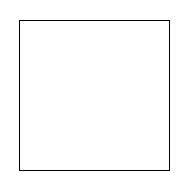
\includegraphics{square}
\end{center}

\index{size@\inlinecode=size=}
通常直接以 \prgname{PostScript} 坐标工作是不方便的。下面的例子绘制一个放缩到
宽 $101$\,bp 和高 $101$\,bp 的单位正方形。其输出与前面的例子相同。
\begin{lstlisting}
size(101,101);
draw((0,0)--(1,0)--(1,1)--(0,1)--cycle);
\end{lstlisting}

\index{unitsquare@\inlinecode=unitsquare=}
为方便计,路径 |(0,0)--(1,0)--(1,1)--(0,1)--cycle| 可以用预定义的变量
|unitsquare| 代换,或等价地,|box((0,0),(1,1))|。

\index{pt@\inlinecode=pt=}
\index{cm@\inlinecode=cm=}
\index{mm@\inlinecode=mm=}
\index{inch@\inlinecode=inch=}
\index{inches@\inlinecode=inches=}
\index{size@\inlinecode=size=}
可以按 |pt|($1$\,|pt|${}=1/72.27$\,|inch|)、|cm|、|mm| 或是 |inches|%
\transnote{这里 \inlinecode{inch} 和 \inlinecode{inches} 意义相同,都是
英尺。}来设定尺寸。如果给定尺寸(|size|)参数为 0,则该方向没有约束;总的放缩
将由另一方向决定(见 \pageref{sec:framepicture} 页 \ref{sec:framepicture} 节
|size| 函数说明):
\lstinputlisting{bigsquare.asy}
\begin{center}
  \includegraphics{bigsquare.pdf}
\end{center}

\index{unitsize@\inlinecode=unitsize=}
要使用户坐标表示正好 |1cm| 的倍数:
\begin{lstlisting}
unitsize(1cm);
draw(unitsquare);
\end{lstlisting}

还可以设定不同的 $x$ 与 $y$ 单位尺寸:
\begin{lstlisting}
unitsize(1cm,2cm);
draw(unitsquare);
\end{lstlisting}

\index{标签}
\index{label@\inlinecode=label=}
在 \prgname{Asymptote} 中很容易增加标签;用双引号引起的 \LaTeX{} 字符串、坐标
和可选的对齐方向来设定标签:
\lstinputlisting{labelsquare.asy}
\begin{center}
  \includegraphics{labelsquare.pdf}
\end{center}

\index{罗盘方向}
\index{E@\inlinecode=E=}
\index{N@\inlinecode=N=}
\index{NE@\inlinecode=NE=}
\index{ENE@\inlinecode=ENE=}
\index{up@\inlinecode=up=}
\index{down@\inlinecode=down=}
\index{right@\inlinecode=right=}
\index{left@\inlinecode=left=}
\prgname{Asymptote} 使用标准的罗盘方向 |E=(1,0)|、|N=(0,1)|、|NE=unit(N+E)|
以及 |ENE=unit(E+NE)| 等等,并在 \prgname{Asymptote} 基本模块 \prgname{plain}
中定义有复数(|pair|) |up|、|down|、|right| 和 |left|。具有名为 |E| 的局部
变量的用户可以通过在前面缀以定义它的模块名来访问罗盘方向 |E|:|plain.E|。

这个例子绘制一条路径近似为 $1/4$ 圆:
\lstinputlisting{quartercircle.asy}
\begin{center}
  \includegraphics{quartercircle.pdf}
\end{center}

\index{--@\inlinecode=--=}
\index{..@\inlinecode=..=}
\index{cycle@\inlinecode=cycle=}
\index{unitcircle@\inlinecode=unitcircle=}
\index{环形路径}
一般地,一条路径由一列复数(或其他路径)确定,它们以 |--| 相连来表示直线段或
|..| 表示三次样条。设定终止结点 |cycle| 建立一条平滑连回初始结点的环形路径,
如在这里对单位圆的近似(精确到 $0.06\%$ 以内):
\begin{lstlisting}
path unitcircle=E..N..W..S..cycle;
\end{lstlisting}

\index{三次样条曲线}
\index{结点}
\index{入向切线}
\index{出向切线}
三次样条曲线的每个内结点可以指定一个前缀或后缀的方向 |{dir}|:复数 |dir| 的
方向分别设定该曲线在此结点处,入向或出向切线的方向。外结点仅能在向内一边指定
方向限定。

\index{控制点}
\index{Bézier 曲线}
在带有后控制点 $c_0$ 的结点 $z_0$,与带有前控制点 $c_1$ 的结点 $z_1$ 之间的
一段三次样条曲线,按 Bézier 曲线
\begin{equation*}
  (1-t)^3 z_0 + 3t(1-t)^2 c_0 + 3t^2 (1-t) c_1 + t^3 z_1, \qquad 0\leq t\leq 1
\end{equation*}
计算\transnote{本节关于三次 Bézier 样条曲线的讲解是比较难懂的,并且下图中关
于曲线离散生成的知识事实上与绘图无关。关于曲线控制的更清晰详细的介绍可以参考
\MP{} 的手册 \textit{\MP{}: A User's Manual} 第 4 章 Curves,以及关于 \MP{} 
与 Con\TeX{}t 的文档 \textit{METAFUN} 的第 1 章。}。

\index{Bézier 曲线!离散生成}
如下图所示,由两个终点 $z_0$ 和 $z_1$ 以及两个控制点 $c_0$ 与 $c_1$ 构造的
三阶中点($m_5$),正是在由四元组 $(z_0, c_0, c_1, z_1)$ 建立的 Bézier 曲线
上对应于 $t = 1/2$ 的点。这就允许人们通过将重新提取的三阶中点用作终点,并
将二阶与一阶中点用作控制点,递归地构造想要的曲线:
\begin{center}
  \includegraphics{bezier2.pdf}
\end{center}
这里 $m_0$, $m_1$ 和 $m_2$ 是一阶中点,$m_3$ 与 $m_4$ 是二阶中点,而 $m_5$ 是
三阶中点。于是曲线就通过对 $(z_0, m_0, m_3, m_5)$ 和 $(m_5, m_4, m_2, z_1)$
递归应用此算法构造出来。

事实上,类似的性质对于每小段中在 $[0,1]$ 上的任意分数 $t$ 位置的点都成立,而
不仅仅是中点($t=1/2$)。

\index{Bézier 曲线!的几何性质}
用这种方式构造的 Bézier 曲线具有如下性质:
\begin{itemize}
  \item 它完全包含在给定四个点的凸包内。
  \item 其起点朝向从第一个端点到第一个控制点而其终点朝向从第二个控制点到
    第二个端点。
\end{itemize}

\index{controls@\inlinecode=controls=}
用户可以像这样设定两个结点间的显式控制点:
\begin{lstlisting}
draw((0,0)..controls (0,100) and (100,100)..(100,0));
\end{lstlisting}

然而,通常更为方便的是仅使用 |..| 运算符,它告诉 \prgname{Asymptote} 使用在
Donald Knuth 的专著 \textit{The \MF{}book} 的第 14 章中描述的算法来选择自己的
控制点。用户还可以通过设定方向、张力和卷曲值来定制路向(或路径)。

\index{张力}
张力越强,曲线越直,它也就越接近直线。可以将样条曲线的张力从其默认值 $1$ 变为
任意大于等于 $0.75$ 的实数值(参考 John D.~Hobby, \textit{Discrete and
Computational Geometry 1}, 1986):
\index{tension@\inlinecode=tension=}
\index{tension atleast@\inlinecode=tension atleast=}
\begin{lstlisting}
draw((100,0)..tension 2 ..(100,100)..(0,100));
draw((100,0)..tension 2 and 1 ..(100,100)..(0,100));
draw((100,0)..tension atleast 1 ..(100,100)..(0,100));
\end{lstlisting}

\index{卷曲参数}
卷曲参数设定在路径端点处的弯曲程度($0$ 表示直的;默认值 $1$ 表示近似为圆):
\index{curl@\inlinecode=curl=}
\begin{lstlisting}
draw((100,0){curl 0}..(100,100)..{curl 0}(0,100));
\end{lstlisting}

\index{::@\inlinecode=::=}
\MP{} 的 |...| 路径连接符,在可能时它要求一个限定在由端点和方向定义的三角形内
的无拐点的曲线,它在 \prgname{Asymptote} 中实现为 |.. tension atleast 1 ..|
的方便缩写 |::|(省略号 |...| 在 \prgname{Asymptote} 中用于标示可变长参数;见
\pageref{subsec:restarguments} 页 \ref{subsec:restarguments} 节剩余参数)。
例如,比较
\lstinputlisting{dots.asy}
\begin{center}
  \includegraphics{dots.pdf}
\end{center}
与
\lstinputlisting{colons.asy}
\begin{center}
  \includegraphics{colons.pdf}
\end{center}

\index{---@\inlinecode=---=}
\index{&@\inlinecode=&=}
|---| 连接符是 |..tension atleast infinity..| 的缩写\transnote{它的效果和通常
的折线连接基本相同,只是在弯折处比完全的折线更为圆滑。},而 |&| 连接符连结两条
路径,并去除第一条路径的第最后一个结点(它一般应该与第二条路径的第一个结点
重合)。

\index{^^@\inlinecode=^^=}
一条相连的 \prgname{Asymptote} 路径,与一条 \prgname{PostScript} 的
\verb=subpath=(子路径)等价。|^^| 二元运算符,它要求画笔从左边路径的终点移动
(而不绘制出来或影响终点的曲率)到右边路径的起点,可以用来将若干
\prgname{Asymptote} 路径聚集到一个 |path[]| 数组中(等价于一条
\prgname{PostScript} 路径):
\lstinputlisting{superpath.asy}
\begin{center}
  \includegraphics{superpath.pdf}
\end{center}

\index{evenodd@\inlinecode=evenodd=}
\index{zerowinding@\inlinecode=zerowinding=}
这里 \prgname{PostScript} 奇偶(|evenodd|)填充规制设定仅在两个圆\transnote{%
原文误作单位圆。事实上这里其中一个圆已经放缩过。}之间界定的区域会被填充。在
这个例子中,如果小心地变换路径的方向,可以使用默认的零卷绕数(|zerowinding|)
填充规则得到同样的效果:
\begin{lstlisting}
filldraw(unitcircle^^reverse(g),yellow,black);
\end{lstlisting}
\index{^^@\inlinecode=^^=}
|^^| 运算符被 \prgname{three.asy} 中的 |box(triple, triple)| 函数用于无回溯
步骤地构造立方体 |unitbox| 的边:
\lstinputlisting{cube.asy}
\begin{center}
  
\includegraphics{cube.pdf}
\end{center}

见原手册 7.25 节 graph 模块\transnote{本译本未包括此节。}(或在线的
\prgname{Asymptote} 画廊和在 \url{http://asymptote.sourceforge.net} 发布的
外部链接)以得到更多例子,包括二维和三维的科学图形。额外的例子则由 Philippe
Ivaldi 在 \url{http://piprim.tuxfamily.org/asymptote/} 发布。



\chapter{绘图命令}
% 4 Drawing commands
\label{chap:drawingcommands}

\prgname{Asymptote} 的全部绘图功能都基于四个基本命令。三个
\prgname{PostScript} 绘图命令 |draw|、|fill| 和 |clip| 按执行顺序将对象加入
图,最近绘制的对象出现在顶层。标注命令 |label| 可用来添加文字标签和外部 EPS
图像,它会显示在 \prgname{PostScript} 对象的上面(鉴于这通常是人们想要的),
而又会以它们执行的相对次序显示。在一幅图(|picture|)上绘制对象后,图可以由
|shipout| 函数输出(见 \pageref{sec:framepicture} 页
\ref{sec:framepicture} 节 |shipout| 的说明)。

\index{layer@\inlinecode=layer=}
\index{层}
如果需要在标签(或逐字的 \TeX 命令,见 \pageref{sec:framepicture} 页
\ref{sec:framepicture} 节 |tex| 的说明)上面绘制 \prgname{PostScript}
对象,可以使用 |layer| 命令开始一个新的 \prgname{PostScript}/\LaTeX{} 层:
\begin{lstlisting}
void layer(picture pic=currentpicture);
\end{lstlisting}
|layer| 函数给人对象绘制的完全控制。层(layer)依次绘制,最近的层出现在顶层。
在每个层中,标签、图像、逐字 \TeX{} 命令总在该层中 \prgname{PostScript} 对象
之后绘制。

尽管下面一些绘图命令有很多选项,它们都有合理的默认值(例如,图参数默认为
|currentpicture|)。


\section{描绘(draw)}
% 4.1 draw

\index{描绘}
\index{draw@\inlinecode=draw=}
\begin{lstlisting}
void draw(picture pic=currentpicture, Label L="", path g,
          align align=NoAlign, pen p=currentpen,
          arrowbar arrow=None, arrowbar bar=None, margin margin=NoMargin,
          Label legend="", marker marker=nomarker);
\end{lstlisting}
在图 |pic| 上使用画笔 |p| 描绘路径 |g|,并带可选的绘制属性(标签 |L|,显式
标签对齐 |align|,箭头与短杠 |arrow| 和 |bar|,边距 |margin|,图例
(|legend|),以及记号 |marker|。只有一个参数,即路径,是必需的。为方便计,
参数 |arrow| 与 |bar| 可按任何次序限定\transnote{即,不论使用的是
\inlinecode{draw(g, BeginBar, EndArrow)} 还是
\inlinecode{draw(g, EndArrow, BeginBar)},得到的图形效果是一样的。}。参数
|legend| 是构造可选图例项时使用的标签。

\index{None@\inlinecode=None=}
\index{BeginBar@\inlinecode=BeginBar=}
\index{EndBar@\inlinecode=EndBar=}
\index{Bars@\inlinecode=Bars=}
\index{barsize@\inlinecode=barsize=}
\index{短杠}
短杠在标明尺寸时很有用。|bar| 可取值 |None|、|BeginBar|、|EndBar|(或等价地
|Bar|)以及 |Bars|(在路径两端绘制短杠)。每个短杠设定(除了 |None|)将接受
一个可选的实数参数以 \prgname{PostScript} 坐标标明短杠的长度。设置的短杠长度
为 |barsize(pen)|。

\index{None@\inlinecode=None=}
\index{Blank@\inlinecode=Blank=}
\index{BeginArrow@\inlinecode=BeginArrow=}
\index{MidArrow@\inlinecode=MidArrow=}
\index{EndArrow@\inlinecode=EndArrow=}
\index{Arrow@\inlinecode=Arrow=}
\index{Arrows@\inlinecode=Arrows=}
\index{arrowhead@\inlinecode=arrowhead=}
\index{Default@\inlinecode=Default=}
\index{SimpleHead@\inlinecode=SimpleHead=}
\index{HookHead@\inlinecode=HookHead=}
\index{TeXHead@\inlinecode=TeXHead=}
\index{FillDraw@\inlinecode=FillDraw=}
\index{Fill@\inlinecode=Fill=}
\index{NoFill@\inlinecode=NoFill=}
\index{UnFill@\inlinecode=UnFill=}
\index{Draw@\inlinecode=Draw=}
\index{arrowsize@\inlinecode=arrowsize=}
\index{BeginArcArrow@\inlinecode=BeginArcArrow=}
\index{EndArcArrow@\inlinecode=EndArcArrow=}
\index{ArcArrow@\inlinecode=ArcArrow=}
\index{MidArcArrow@\inlinecode=MidArcArrow=}
\index{ArcArrows@\inlinecode=ArcArrows=}
\index{箭头}
|arrow| 可取值 |None|、|Blank|(不画出箭头与路径\transnote{利用它可以只画一组
短杠。})、|BeginArrow|、|MidArrow|、|EndArrow|(或等价地 |Arrow|)以及
|Arrows|(在路径的两端都绘制箭头)。除 |None| 和 |Blank| 外的所有箭头设定可以
给以可选的箭尖参数 |arrowhead|(预定义的箭头风格 |Default|、|SimpleHead|、
|HookHead|、|TeXHead| 之一),实数 |size|(\prgname{PostScript} 坐标的箭尖
尺寸),实数 |angle|(箭尖角度,以度计),填充类型 |filltype|(|FillDraw|、
|Fill|、|NoFill|、|UnFill|、|Draw| 之一)以及(除了 |MidArrow| 和 |Arrows|)
表示箭头顶端沿路径放置相对位置的实数 |position|(一个 |arctime|)。用画笔 |p|
绘制时,默认的箭尖尺寸为 |arrowsize(p)|。还有 |size| 与 |angle| 默认值略有
修改的适合曲线的箭头版本\transnote{其中如果使用 \inlinecode{TeXHead},尺寸过
大,而效果不佳。}:|BeginArcArrow|、|EndArcArrow|(或等价地 |ArcArrow|)、
|MidArcArrow| 以及 |ArcArrows|。

\index{NoMargin@\inlinecode=NoMargin=}
\index{BeginMargin@\inlinecode=BeginMargin=}
\index{EndMargin@\inlinecode=EndMargin=}
\index{Margins@\inlinecode=Margins=}
\index{Margin@\inlinecode=Margin=}
\index{labelmargin@\inlinecode=labelmargin=}
\index{BeginPenMargin@\inlinecode=BeginPenMargin=}
\index{EndPenMargin@\inlinecode=EndPenMargin=}
\index{PenMargin@\inlinecode=PenMargin=}
\index{PenMargins@\inlinecode=PenMargins=}
\index{DotMargin@\inlinecode=DotMargin=}
\index{dotfactor@\inlinecode=dotfactor=}
\index{BeginDotMargin@\inlinecode=BeginDotMargin=}
\index{EndDotMargin@\inlinecode=EndDotMargin=}
\index{DotMargins@\inlinecode=DotMargins=}
\index{TrueMargin@\inlinecode=TrueMargin=}
\index{边距}
边距可以用于收缩 |labelmargin(p)| 长的路径可见部分以避免与其他画出的对象
重叠。|margin| 的典型值为 |NoMargin|、|BeginMargin|、|EndMargin|(或等价地
|Margin|)以及 |Margins|(它在路径的两端都留下边距)。可以使用
|Margin(real begin, real end)|,以用于对齐标签的单位 |labelmargin(p)| 的倍数
来分别设定起始和终点的边距大小。此外,|BeginPenMargin|、|EndPenMargin|(或
等价地 |PenMargin|)、|PenMargins|、|PenMargin(real begin, real end)| 以画笔
线宽为单位确定边距,这里考虑在绘制路径或箭头时的画笔线宽。例如,使用
|DotMargin|,即 |PenMargin(-0.5*dotfactor,0.5*dotfactor)| 的缩写,来绘制从
通常的起点恰好到达宽度为 |dotfactor*linewidth(p)| 的终点的边界。修饰符
|BeginDotMargin|、|EndDotMargin| 和 |DotMargins| 与之类似。修饰符
|TrueMargin(real begin, real end)| 允许人们直接用 \prgname{PostScript} 单位
设定边距,而与画笔的线宽无关。

箭头、短杠和边距的用法在示例文件 \prgname{Pythagoras.asy}、%
\prgname{sqrtx01.asy} 和 \prgname{triads.asy} 中展示%
\transnote{\label{foot:pythagoras}这里仅给出 \prgname{Pythagoras.asy} 例子的
效果,代码略:\begin{center}
  \includegraphics[height=5\baselineskip]{Pythagoras}
\end{center}}。

\index{图例}
一幅图 |pic| 的图例可以用下列过程对齐装入一帧:
\index{legend@\inlinecode=legend=}
\begin{lstlisting}
frame legend(picture pic=currentpicture, int perline=1,
             real xmargin=legendmargin, real ymargin=xmargin,
             real linelength=legendlinelength,
             real hskip=legendhskip, real vskip=legendvskip,
             real maxwidth=0, real maxheight=0,
             bool hstretch=false, bool vstretch=false, pen p=currentpen);
\end{lstlisting}
这里 |xmargin| 与 |ymargin| 设定四周 $x$ 与 $y$ 边距,|perline| 设定每行的
条目数(默认为 1;0 表示自动选取此数目),|linelength| 设定路径线的长度,
|hskip| 与 |vskip| 设定行距(按图例条目尺寸的倍数),|maxwidth| 与
|maxheight| 设定可选的最终图例长宽上界(0 表示无限定),|hstretch| 和
|vstretch| 允许图例在水平和竖直方向伸缩,而 |p| 设定用于绘制边框的画笔。图例
的帧于是可以使用 |add| 和 |attach| 添加进来并相对图 |dest| 上一点对齐(参看
\pageref{sec:framepicture} 页 \ref{sec:framepicture} 节 |add| 函数)。

\index{画点}
\index{dotfactor@\inlinecode=dotfactor=}
要绘制一点,只要画出只包含一个单独点的路径。在 |plain| 模块中定义的命令 |dot|
画出一个点,它有等于显式画笔线宽或默认线宽放大 |dotfactor|(默认为 6)倍的
直径,并使用设定的填充类型(见 \pageref{sec:framepicture} 页
\ref{sec:framepicture} 节填充类型的说明):
\index{dot@\inlinecode=dot=}
\begin{lstlisting}
void dot(picture pic=currentpicture, pair z, pen p=currentpen,
         filltype filltype=Fill);
void dot(picture pic=currentpicture, Label L, pair z, align align=NoAlign,
         string format=defaultformat, pen p=currentpen, filltype filltype=Fill);
void dot(picture pic=currentpicture, Label[] L=new Label[], pair[] z,
         align align=NoAlign, string format=defaultformat, pen p=currentpen,
         filltype filltype=Fill)
void dot(picture pic=currentpicture, Label L, pen p=currentpen,
         filltype filltype=Fill);
\end{lstlisting}
\index{defaultformat@\inlinecode=defaultformat=}
如果给定变量 |Label| 为第二个过程的 |Label| 参数,|format| 参数将用于在格式化
打点位置的字符串(这里默认值 |defaultformat| 为 |"$%.4g$"|)。
\iffalse$\fi  % 欺骗编辑器语法高亮
\index{画路径上的点}
第三个过程在复数数组 |z| 的每个点处画一个点。还可以在一条路径的每个结点处打
一个点:
\index{dot@\inlinecode=dot=}
\begin{lstlisting}
void dot(picture pic=currentpicture, Label[] L=new Label[],
         path g, align align=RightSide, string format=defaultformat,
         pen p=currentpen, filltype filltype=Fill);
\end{lstlisting}
参看原手册 7.25 节 \prgname{graph} 模块和 7.8 节 \prgname{markers} 模块%
\transnote{本译本未包括此部分。}中给路径结点标记的更一般的途径。

要关于用户坐标 |origin| 绘制固定尺寸的对象(以 \prgname{PostScript}
坐标),使用过程
\index{draw@\inlinecode=draw=}
\begin{lstlisting}
void draw(pair origin, picture pic=currentpicture, Label L="", path g,
          align align=NoAlign, pen p=currentpen, arrowbar arrow=None,
          arrowbar bar=None, margin margin=NoMargin, Label legend="",
          marker marker=nomarker);
\end{lstlisting}



\section{填充(fill)}
% 4.2 fill
\label{sec:fill}

\index{填充}
\index{fill@\inlinecode=fill=}
\begin{lstlisting}
void fill(picture pic=currentpicture, path g, pen p=currentpen);
\end{lstlisting}
使用画笔 |p|,在图 |pic| 上填充由环形路径 |g| 限定的区域内部。

\index{filldraw@\inlinecode=filldraw=}
还有一个方便的 |filldraw| 命令,它填充路径并绘制边界线。可以为每个操作分别
设定画笔:
\begin{lstlisting}
void filldraw(picture pic=currentpicture, path g, pen fillpen=currentpen,
              pen drawpen=currentpen);
\end{lstlisting}

\index{fill@\inlinecode=fill=}
这个固定尺寸的 |fill| 版本允许人们填充一个关于用户坐标 |origin|,以
\prgname{PostScript} 坐标描述的对象:
\begin{lstlisting}
void fill(pair origin, picture pic=currentpicture, path g, pen p=currentpen);
\end{lstlisting}
这只不过是如下命令的方便缩写:
\begin{lstlisting}
picture opic;
fill(opic,g,p);
add(pic,opic,origin);
\end{lstlisting}

过程
\index{filloutside@\inlinecode=filloutside=}
\begin{lstlisting}
void filloutside(picture pic=currentpicture, path g, pen p=currentpen);
\end{lstlisting}
填充路径 |g| 的区域外部,向外直达图 |pic| 的当前边界。

\index{渐变!格状梯度光滑渐变}
在二维画笔数组 |p| 之上使用填充规则 |fillrule| 的格状梯度光滑渐变,可以由
\index{latticeshade@\inlinecode=latticeshade=}
\begin{lstlisting}
void latticeshade(picture pic=currentpicture, path g, bool stroke=false,
                  pen fillrule=currentpen, pen[][] p);
\end{lstlisting}
产生。如果 |stroke=true|,填充区域就与由 |draw(pic,g,fillrule+zerowinding)|
绘制的区域相同\transnote{即这里填充的是具有宽度的路径本身。};在这种情况下,
路径 |g| 不必是环形的。|p| 中的画笔必须属于同一颜色空间。可以使用函数
|rgb(pen)| 或 |cmyk(pen)| 来将画笔提升到一个较高的颜色空间,如在示例文件
\prgname{latticeshading.asy} 中展示的那样\transnote{文档此处和实际行为不符,
从早期版本开始,\inlinecode{latticeshade} 就一直会自动进行颜色空间的提升,从
灰阶到 RGB 到 CMYK,因而 \inlinecode{p} 参数不需要手工提升到同一颜色空间。
参看示例文件 \prgname{latticeshading.asy}:\\
\setbox0\vbox{\lstinputlisting{latticeshading.asy}}%
\includegraphics[height=\ht0]{latticeshading.pdf}\box0}。

\index{渐变!轴向梯度光滑渐变}
按线段 |a--b| 方向,从画笔 |pena| 到 |penb| 的轴向梯度光滑渐变可以由下面函数
得到\transnote{这里给一个例子:\\
\setbox0\vbox{\lstinputlisting{axialshade.asy}}%
\includegraphics[height=\ht0]{axialshade.pdf}\box0}:
\index{axialshade@\inlinecode=axialshade=}
\begin{lstlisting}
void axialshade(picture pic=currentpicture, path g, bool stroke=false,
                pen pena, pair a,
                pen penb, pair b);
\end{lstlisting}

\index{渐变!放射梯度光滑渐变}
从以 |a| 圆心 |ra| 为半径的圆上的画笔 |pena|,到以 |b| 为圆心 |rb| 为半径的
圆上的画笔 |penb| 的放射梯度光滑渐变,也是类似的:
\index{radialshade@\inlinecode=radialshade=}
\begin{lstlisting}
void radialshade(picture pic=currentpicture, path g, bool stroke=false,
                 pen pena, pair a, real ra,
                 pen penb, pair b, real rb);
\end{lstlisting}
放射渐变的例子在示例文件 \prgname{shade.asy}、\prgname{ring.asy} 和
\prgname{shadestroke.asy} 中\transnote{仅举 \prgname{shadestroke.asy}
一例:\\
\setbox0\vbox{\lstinputlisting{shadestroke.asy}}%
\includegraphics[height=\ht0]{shadestroke.pdf}\box0}。

\index{渐变!Gouraud 渐变}
在由顶点集 |z| 和边标志 |edges| 定义的三角格点上,使用填充规则 |fillrule| 及
画笔数组 |p| 中的顶点颜色的 Gouraud 渐变,由下面函数实现:
\index{gouraudshade@\inlinecode=gouraudshade=}
\begin{lstlisting}
void gouraudshade(picture pic=currentpicture, path g, bool stroke=false,
                  pen fillrule=currentpen, pen[] p, pair[] z,
                  int[] edges);
void gouraudshade(picture pic=currentpicture, path g, bool stroke=false,
                  pen fillrule=currentpen, pen[] p, int[] edges);
\end{lstlisting}
在第二种形式中,|z| 的元素取为依次路径 |g| 的各结点。|p| 中的画笔必须属于同一
颜色空间。Gouraud 渐变的例子在示例文件 \prgname{Gouraud.asy} 和实体几何模块
\prgname{solids.asy} 中提供\transnote{\inlinecode{p} 中画笔事实上会被自动提升
到同一颜色空间。\prgname{Gouraud.asy} 的效果如下(代码略):\\
\centerline{\includegraphics[scale=0.6]{Gouraud.pdf}}}。用于 Gouraud 渐变的
边标志的文档见
\url{http://partners.adobe.com/public/developer/en/ps/sdk/TN5600.SmoothShading.pdf}。

\index{渐变!张量积渐变}
在由路径数组 |b| 中的长度为 4 的 $n$ 环形路径界定的补片上,使用由 $n\times4$
的画笔数组 |p| 和 $n\times4$ 数组内的中间控制点确定的顶点颜色,使用填充规则
|fillrule| 的张量积渐变,由下面函数实现:
\index{tensorshade@\inlinecode=tensorshade=}
\begin{lstlisting}
void tensorshade(picture pic=currentpicture, path g, bool stroke=false,
                 pen fillrule=currentpen, pen[][] p, path[] b=g,
                 pair[][] z=new pair[][]);
\end{lstlisting}
\index{渐变!Coons 渐变}
如果数组 |z| 为空,将使用 Coons 渐变,其中颜色控制点会自动计算。|p| 中画笔
必须属于同一颜色空间。对只有单个补片($n=1$)的情形的更简单的界面也是可用的:
\index{tensorshade@\inlinecode=tensorshade=}
\begin{lstlisting}
void tensorshade(picture pic=currentpicture, path g, bool stroke=false,
                 pen fillrule=currentpen, pen[] p, path b=g,
                 pair[] z=new pair[]);
\end{lstlisting}
\index{渐变!填充连续一列路径之间的区域}
还可以使用给定的画笔数组,光滑渐变填充连续一列路径之间的区域:
\index{draw@\inlinecode=draw=}
\begin{lstlisting}
void draw(picture pic=currentpicture, path[] g, pen[] p);
\end{lstlisting}
张量积和 Coons 渐变的例子在示例文件 \prgname{tensor.asy}、
\prgname{Coons.asy}、\prgname{BezierSurface.asy} 和 \prgname{rainbow.asy}
中\transnote{这里仅举出最简单的 Coons 渐变的例子:\\
\setbox0\vbox{\lstinputlisting{Coons.asy}}%
\includegraphics[height=\ht0]{Coons.pdf}\box0}。

\index{渐变!函数式渐变}
用 pdf\LaTeX, \ConTeXt{} 和 pdf\TeX{} 的 \TeX{} 引擎可得到更一般的渐变的可能:
过程
\index{functionshade@\inlinecode=functionshade=}
\begin{lstlisting}
void functionshade(picture pic=currentpicture, path[] g, bool stroke=false,
                   pen fillrule=currentpen, string shader);
\end{lstlisting}
使用由字符串 |shader| 设定的 \prgname{PostScript} 计算过程,按填充规则
|fillrule|,在图 |pic| 上路径 |g| 内部的部分做渐变填充;该
(\prgname{PostScript})过程取 2 个参数,各自在 $[0,1]$ 取值,并返回
|colors(fillrule).length| 个颜色成分。函数式渐变在例子
\prgname{functionshading.asy} 中示例。

\index{反填充}
下面的过程使用 |evenodd| 剪裁连同 |^^| 运算符来反填充一个区域:
\index{unfill@\inlinecode=unfill=}
\begin{lstlisting}
void unfill(picture pic=currentpicture, path g);
\end{lstlisting}


\section{剪裁(clip)}
% 4.3 clip

\index{剪裁}
\index{clip@\inlinecode=clip=}
\begin{lstlisting}
void clip(picture pic=currentpicture, path g, stroke=false,
          pen fillrule=currentpen);
\end{lstlisting}
使用填充规则 |fillrule|(见 \pageref{sec:pens} 页 \ref{sec:pens} 节),把图
|pic| 当前的内容按路径 |g| 界定的区域剪裁。如果 |stroke=true|,剪裁的部分与
|draw(pic,g,fillrule+zerowinding)| 绘制的区域相同;在这种情况下路径 |g| 不必
是环形的。图剪裁的例子,见原手册第 6 章 \LaTeX\ usage 的第一个例子\transnote{
本译本未包含此章。这里另给一个简单的例子:\\
\setbox0\vbox{\lstinputlisting{clippath.asy}}%
\includegraphics[height=\ht0]{clippath.pdf}\box0}。


\section{标注(label)}
% 4.4 label
\label{sec:label}

\index{标注}
\index{label@\inlinecode=label=}
\begin{lstlisting}
void label(picture pic=currentpicture, Label L, pair position,
           align align=NoAlign, pen p=nullpen, filltype filltype=NoFill)
\end{lstlisting}
\index{align@\inlinecode=ailgn=}
\index{NoAlign@\inlinecode=NoAlign=}
\index{labelmargin@\inlinecode=labelmargin=}
\index{Align@\inlinecode=Align=}
\index{标签}
\index{对齐}
使用画笔 |p| 在图 |pic| 上绘制标签 |L|。如果 |align| 为 |NoAlign|,标签将在
用户坐标 |position| 居中;否则将以 |align| 方向从 |position| 以
\prgname{PostScript} 坐标偏移 |align*labelmargin(p)| 的距离对齐。常数 |Align|
可以用来按标签的左下角在 |position| 位置对齐。如果 |p| 为 |nullpen|,在标签中
设定的画笔(默认为 |currentpen|)将被使用。标签 |L| 既可以是一个字符串也可以
是通过调用如下函数之一得到的结构体:
\index{Label@\inlinecode=Label=}
\begin{lstlisting}
Label Label(string s="", pair position, align align=NoAlign,
            pen p=nullpen, embed embed=Rotate, filltype filltype=NoFill);
Label Label(string s="", align align=NoAlign,
            pen p=nullpen, embed embed=Rotate, filltype filltype=NoFill);
Label Label(Label L, pair position, align align=NoAlign,
            pen p=nullpen, embed embed=L.embed, filltype filltype=NoFill);
Label Label(Label L, align align=NoAlign,
            pen p=nullpen, embed embed=L.embed, filltype filltype=NoFill);
\end{lstlisting}
标签的文字可以通过左乘一个仿射变换(见 \pageref{sec:transforms} 页
\ref{sec:transforms} 节)而被放缩、倾斜、旋转或是平移。例如,%
|rotate(45)*xscale(2)*L| 首先在 $x$ 方向放缩 |L| 而后将其逆时针方向旋转
$45^\circ$。标签的最终位置还可以通过 \prgname{PostScript} 坐标转换平移:%
|shift(10,0)*L|。|embed| 参数决定标签如何随着嵌入(此标签的)图变换:
\begin{funclist}
\index{Shift@\inlinecode=Shift=}
\item |Shift| \go
  仅随嵌入它的图平移;
\index{Rotate@\inlinecode=Rotate=}
\item |Rotate| \go
  仅随嵌入它的图平移和旋转(默认值);
\index{Rotate@\inlinecode=Rotate=}
\item |Rotate(pair z)| \go
  按(随图变换过的)向量 |z| 旋转;
\index{Slant@\inlinecode=Slant=}
\item |Slant| \go
  仅随嵌入它的图平移、旋转、倾斜、反射;
\index{Scale@\inlinecode=Scale=}
\item |Scale| \go
  随嵌入它的图的平移、旋转、倾斜、反射和放缩;
\end{funclist}

\index{标注路径}
要给一条路径加标签,用
\index{label@\inlinecode=label=}
\begin{lstlisting}
void label(picture pic=currentpicture, Label L, path g, align align=NoAlign,
           pen p=nullpen, filltype filltype=NoFill);
\end{lstlisting}
\index{标签位置}
\index{position@\inlinecode=position=}
\index{Relative@\inlinecode=Relative=}
标签默认将位于路径的中点。另一种标签位置(一个在 0 与 |length(g)| 之间的
|arctime| 值,参看 \pageref{sec:pathsandguides} 页 \ref{sec:pathsandguides}
节 |arctime| 函数)可以在构造标签时用一个实数值 |position| 设定。位置
|Relative(real)| 确定一个相对于路径总弧长的位置\transnote{\label{foot:morelabel}
因而除了上面的提及的四种 \inlinecode{Label} 构造函数外,还有两种接受
\inlinecode{position} 类型参数的构造函数:
\begin{lstlisting}^^J
Label Label(string s, string size="", explicit position position,^^J
\ \ \ \ \ \ \ \ \ \ \ \ align align=NoAlign, pen p=nullpen, embed embed=Rotate,^^J
\ \ \ \ \ \ \ \ \ \ \ \ filltype filltype=NoFill);^^J
Label Label(Label L, explicit position position, align align=NoAlign,^^J
\ \ \ \ \ \ \ \ \ \ \ \ pen p=nullpen, embed embed=L.embed, filltype filltype=NoFill);^^J
\end{lstlisting}
其 \inlinecode{position} 参数即可以是一个实数,也可以是一个
\inlinecode{Relative(value)} 值。}。如下的方便缩写形式已经预定义好了:
\index{BeginPoint@\inlinecode=BeginPoint=}
\index{MidPoint@\inlinecode=MidPoint=}
\index{EndPoint@\inlinecode=EndPoint=}
\begin{lstlisting}
position BeginPoint=Relative(0);
position MidPoint=Relative(0.5);
position EndPoint=Relative(1);
\end{lstlisting}
\index{align@\inlinecode=align=}
\index{对齐}
\index{Relative@\inlinecode=Relative=}
路径标签以方向 |align| 对齐,它可由一个绝对罗盘方向(复数 |pair|)或相对于
路径本地方向北极轴测量的方向 |Relative(pair)| 设定\transnote{%
\inlinecode{Relative(N)} 就是路径在此位置的切向。有关这种 \inlinecode{Label}
的 \inlinecode{position} 和 \inlinecode{align} 参数的意义,如图所示:
\begin{center}\includegraphics{labelalign.pdf}\end{center}}。
\index{LeftSide@\inlinecode=LeftSide=}
\index{Center@\inlinecode=Center=}
\index{RightSide@\inlinecode=RightSide=}
为方便计,|LeftSide|、|Center| 和 |RightSide| 分别定义为 |Relative(W)|、%
|Relative((0,0))| 以及 |Relative(E)|。给 |LeftSide|、|Center| 和 |RightSide|
左乘一个实数放缩因子会把标签移得更靠近或更远离路径\transnote{除了上文和脚注
\ref{foot:morelabel} 中的六种 \inlinecode{Label} 构造函数,在 \prgname{plain}
模块中还有一种构造函数,它将标签位置(复数 \inlinecode{pair} 类型)自动转换为
标签的内容:
\begin{lstlisting}^^J
Label Label(pair position, align align=NoAlign, pen p=nullpen,^^J
\ \ \ \ \ \ \ \ \ \ \ \ embed embed=Rotate, filltype filltype=NoFill);^^J
\end{lstlisting}}。

\index{arrowlength@\inlinecode=arrowlength=}
带有从方向 |dir| 来指向 |b| 的长为 |arrowlength| 的固定尺寸箭头的标签,可以由
如下过程产生:
\index{arrow@\inlinecode=arrow=}
\begin{lstlisting}
void arrow(picture pic=currentpicture, Label L="", pair b, pair dir,
           real length=arrowlength, align align=NoAlign,
           pen p=currentpen, arrowbar arrow=Arrow, margin margin=EndMargin);
\end{lstlisting}
如果没有设定对齐方向(不论是在标签中还是明确以参数给出),可选的标签将使用
边距 |align|,以 |dir| 的方向对齐。

\index{graphic@\inlinecode=graphic=}
函数 |string graphic(string name, string options="")| 返回一个可以用于插入
嵌入式 \prgname{PostScript}(Encapsulated \prgname{PostScript},EPS)文件的
字符串。这里,|name| 是要插入的文件名而 |options| 是一个逗号分隔的参数列表
字符串:包括可选的边框(|bb=llx lly urx ury|)、宽度(|width=value|)、高度
(|height=value|)、旋转(|angle=value|)、放缩(|scale=factor|)、剪裁
(|clip=bool|)以及草稿模式(|draft=bool|)。|layer()| 函数可用来强迫将来的
对象在插入的图像上方绘制:
\begin{lstlisting}
label(graphic("file.eps","width=1cm"),(0,0),NE);
layer();
\end{lstlisting}

\index{baseline@\inlinecode=baseline=}
\index{基线}
|string baseline(string s, string template="\strut")| 函数可用于
扩大标签的边框以匹配给定的模板,从而这些标签的基线将排在同一水平线上。
参见 \prgname{Pythagoras.asy} 的例子\transnote{\prgname{Pythagoras.asy}
的例子见脚注 \ref{foot:pythagoras}。}。

\index{overwrite@\inlinecode=overwrite=}
用 |overwrite| 画笔属性(参看 \pageref{sec:pens} 页 \ref{sec:pens} 节),可以
避免标签互相覆写。

\index{object@\inlinecode=object=}
在 \prgname{plain\_Label.asy} 中定义的结构体 |object|(对象)允许以一致的行为
方式看待标签和帧。用如下过程可以将一组对象打包进一帧内:
\index{pack@\inlinecode=pack=}
\begin{lstlisting}
frame pack(pair align=2S ... object inset[]);
\end{lstlisting}
要绘制或填充围绕一个标签的方盒(或是椭圆或其他路径)并返回界定的对象,使用
如下过程之一:
\index{draw@\inlinecode=draw=}
\begin{lstlisting}
object draw(picture pic=currentpicture, Label L, envelope e,
            real xmargin=0, real ymargin=xmargin, pen p=currentpen,
            filltype filltype=NoFill, bool above=true);
object draw(picture pic=currentpicture, Label L, envelope e, pair position,
            real xmargin=0, real ymargin=xmargin, pen p=currentpen,
            filltype filltype=NoFill, bool above=true);
\end{lstlisting}
\index{envelope@\inlinecode=envelope=}
\index{box@\inlinecode=box=}
\index{roundbox@\inlinecode=roundbox=}
\index{ellipse@\inlinecode=ellipse=}
这里 |envelope| 是在 \prgname{plain\_boxes.asy} 中定义的边界绘制过程(参看
\pageref{sec:pathsandguides} 页 \ref{sec:pathsandguides} 节),如 |box|、
|roundbox| 或 |ellipse|。

\index{texpath@\inlinecode=texpath=}
函数 |path[] texpath(Label L)| 返回 \TeX{} 将要为绘制标签 |L| 而填充的路径。

\index{minipage@\inlinecode=minipage=}
函数 |string minipage(string s, width=100pt)| 可用于将字符串 |s| 格式化为一个
宽度为 |width| 的段落。这个例子利用 |minipage|、|clip| 和 |graphic| 来生成一
个 CD 标签:
\begin{center}
  \includegraphics{CDlabel.pdf}
\end{center}
\lstinputlisting{CDlabel.asy}


\chapter{编程}
% 5 Programming
\label{chap:programming}

\index{控制结构}
\index{控制流}
这里是对程序设计语言 \prgname{Asymptote} 的一个介绍性的例子,强调其中与
C, C++ 和 Java 相似的控制结构\transnote{这个文档无疑是面向具有 C, C++ 或 Java
等语言编程经验的人的,因而这里关于控制流的说明简略得甚至有些过分,比如没有
给出 \inlinecode{do} 结构的例子。有需要的读者请参考相关语言和程序设计的其他
书籍。}。

\index{注释}
\index{//@\inlinecode=//=}
\index{/* */@\inlinecode=/* */=}
\index{声明变量}
\index{条件测试}
\index{if@\inlinecode=if=}
\index{else@\inlinecode=else=}
\index{循环}
\index{for@\inlinecode=for=}
\begin{lstlisting}
// 这是一行注释。

// 声明:声明 x 是一个 real 变量;
real x;

// 赋值:给 real 变量 x 赋值 1 。
x=1.0;

// 条件:测试 x 是否等于 1 。
if(x == 1.0) {
  write("x 等于 1.0");
} else {
  write("x 不等于 1.0");
}

// 循环:迭代 10 次
for(int i=0; i < 10; ++i) {
  write(i);
}
\end{lstlisting}

\index{while@\inlinecode=while=}
\index{do@\inlinecode=do=}
\index{break@\inlinecode=break=}
\index{continue@\inlinecode=continue=}
正如在 C/C++ 中一样,\prgname{Asymptote} 支持 |while|, |do|, |break| 和
|continue| 语句。Java 风格的迭代遍历数组元素的简便形式也是支持的:
\index{for@\inlinecode=for=}
\index{遍历数组}
\begin{lstlisting}
// 迭代遍历一个数组
int[] array={1,1,2,3,5};
for(int k : array) {
  write(k);
}
\end{lstlisting}
此外,它也支持许多上述语言之外的特征。


\section{数据类型}
% 5.1 Data types

\index{数据类型}
\prgname{Asymptote} 支持下列数据类型(除用户自定义类型外):
\begin{typelist}

\index{void@\inlinecode=void=}
\index{空类型}
\item[void] 空(|void|)类型仅用于无参数或无返回值的函数。

\index{bool@\inlinecode=bool=}
\index{布尔类型}
\index{true@\inlinecode=true=}
\index{false@\inlinecode=false=}
\item[bool] 布尔类型只能取值 |true| 或 |false|。例如:
\begin{lstlisting}
bool b = true;
\end{lstlisting}
定义一个布尔变量 |b| 并初始化为值 |true|。如果没有给定初始式:
\begin{lstlisting}
bool b;
\end{lstlisting}
其值假定为 |false|。

\index{bool3@\inlinecode=bool3=}
\index{扩展布尔类型}
\index{true@\inlinecode=true=}
\index{false@\inlinecode=false=}
\index{default@\inlinecode=default=}
\item[bool3] 一种扩展的布尔类型,可以取值 |true|, |default| 或 |false|。
|bool3| 类型可以与 |bool| 类型相互转换。|bool3| 的默认初始式为 |default|。

\index{int@\inlinecode=int=}
\index{整数}
\index{intMin@\inlinecode=intMin=}
\index{intMax@\inlinecode=intMax=}
\item[int] 整数类型;如果没有给定初始式,隐式的值假定为 |0|。整数允许的最小值
为 |intMin|,最大值为 |intMax|。

\index{real@\inlinecode=real=}
\index{实数}
\index{realEpsilon@\inlinecode=realEpsilon=}
\index{realDigits@\inlinecode=realDigits=}
\index{realMin@\inlinecode=realMin=}
\index{realMax@\inlinecode=realMax=}
\item[real] 实数;它将设为计算机结构的本地浮点类型的最大精度。实数的隐式
初始式为 |0.0|。实数具有精度 |realEpsilon|,有效数字为 |realDigits|。最小的
正实数为 |realMin|,而最大的正实数为 |realMax|。

\index{pair@\inlinecode=pair=}
\index{复数}
\index{x@\inlinecode=x=}
\index{y@\inlinecode=y=}
\index{实部}
\index{虚部}
\item[pair] 复数,即,实数构成的有序对 |(x, y)|。复数 |z| 的实部和虚部可读为
|z.x| 和 |z.y|。我们称 |x| 和 |y| 为复数数据元素的虚拟成员;然而,它们不能
直接修改。复数的隐式初始式为 |(0.0,0.0)|。

有许多方法取复数的复共轭:
\begin{lstlisting}
pair z=(3,4);
z=(z.x,-z.y);
z=z.x-I*z.y;
z=conj(z);
\end{lstlisting}
\index{I@\inlinecode=I=}
这里 |I| 是复数 |(0,1)|。复数类型定义了许多内部函数:
\begin{funclist}
\index{conf@\inlinecode=conf=}
\index{复共轭}
\item |pair conf(pair z)| \go
  返回 |z| 的复共轭。

\index{length@\inlinecode=length=}
\index{模长}
\item |real length(pair z)| \go
  返回参数 |z| 的复数模长 $\vert$|z|$\vert$。例如,
\begin{lstlisting}
pair z=(3,4);
length(z);
\end{lstlisting}
  返回结果 5。|abs(pair)| 与 |length(pair)| 同义;

\index{angle@\inlinecode=angle=}
\index{幅角}
\item |real angle(pair z, bool warn=true)| \go
  返回 |z| 的幅角,单位为弧度,在区间 $[-\uppi, \uppi]$ 内,而当 |warn| 为
  |false| 且 |z|${}={}$|(0,0)| 时返回 |0|(而不是产生错误);

\index{degrees@\inlinecode=degrees=}
\index{幅角}
\item |real degrees(pair z, bool warn=true)| \go
  返回 |z| 的幅角,单位为度,在区间 $[0,360)$ 内,而当 |warn| 为 |false| 且
  |z|${}={}$|(0,0)| 时返回 |0|(而不是产生错误);

\index{unit@\inlinecode=unit=}
\index{单位向量}
\item |pair unit(pair z)| \go
  返回以复数 |z| 同方向的单位向量;

\index{expi@\inlinecode=expi=}
\index{单位向量}
\item |pair expi(real angle)| \go
  返回以弧度角 |angle| 为方向的单位向量;

\index{dir@\inlinecode=dir=}
\index{单位向量}
\item |pair dir(real degrees)| \go
  返回以角度 |degrees| 为方向的单位向量;

\index{xpart@\inlinecode=xpart=}
\index{x 部分@$x$ 部分}
\index{实部}
\item |real xpart(pair z)| \go
  返回 |z.x|;

\index{ypart@\inlinecode=ypart=}
\index{y 部分@$y$ 部分}
\index{虚部}
\item |real ypart(pair z)| \go
  返回 |z.y|;

\index{realmult@\inlinecode=realmult=}
\index{逐元素乘积}
\item |pair realmult(pair z, pair w)| \go
  返回逐元素乘积 |(z.x*w.x,z.y*w.y)|;

\index{dot@\inlinecode=dot=}
\index{点积}
\item |real dot(pair z, pair w)| \go
  返回点积 |z.x*w.x+z.y*w.y|;

\index{minbound@\inlinecode=minbound=}
\item |pair minbound(pair z, pair w)| \go
  返回 |(min(z.x,w.x),min(z.y,w.y))|;

\index{maxbound@\inlinecode=maxbound=}
\item |pair maxbound(pair z, pair w)| \go
  返回 |(max(z.x,w.x),max(z.y,w.y))|。
\end{funclist}

\index{triple@\inlinecode=triple=}
\index{三元组}
\index{x@\inlinecode=x=}
\index{y@\inlinecode=y=}
\index{z@\inlinecode=z=}
\item[triple] 有序实数三元组(向量)|(x,y,z)| 用于三维作图。三元组 |v| 的对应
组成部分分别读为 |v.x|, |v.y| 和 |v.z|。隐式初始式为 |(0.0,0.0,0.0)|。

这里是三元组的内部函数:
\begin{funclist}
\index{length@\inlinecode=length=}
\index{模长}
\item |real length(triple v)| \go
  返回向量 |v| 的长度 $\vert$|v|$\vert$。|abs(triple)| 与 |length(triple)| 同
  义;

\index{polar@\inlinecode=polar=}
\index{余纬角}
\item |real polar(triple v, bool warn=true)| \go
  返回 |v| 的余纬角,从 $z$ 轴计,单位为弧度,而当 |warn| 为 |false| 且
  |v|${}={}$|O| 时\transnote{即 \inlinecode{v} 的所有坐标均为 0。
  \inlinecode{O} 不是内部的常量,而是在 \prgname{three} 模块中定义的变量
  \inlinecode{(0,0,0)}。后同。}返回 |0|(而不是产生错误);

\index{azimuth@\inlinecode=azimuth=}
\index{经度角}
\item |real azimuth(triple v, bool warn=true)| \go
  返回 |v| 的经度角,从 $x$ 轴计,单位为弧度,而当 |warn| 为 |false| 且
  |v.x|${}={}$|v.y|${}={}$|0| 时返回 |0|(而不是产生错误);

\index{colatitude@\inlinecode=colatitude=}
\index{余纬角}
\item |real colatitude(triple v, bool warn=true)| \go
  返回 |v| 的余纬角,从 $z$ 轴计,单位为度,而当 |warn| 为 |false| 且
  |v|${}={}$|O| 时返回 |0|(而不是产生错误);

\index{latitude@\inlinecode=latitude=}
\index{纬度角}
\item |real latitude(triple v, bool warn=true)| \go
  返回 |v| 的纬度角,从 $xy$ 平面计,单位为度,而当 |warn| 为 |false| 且
  |v|${}={}$|O| 时返回 |0|(而不是产生错误);

\index{longitude@\inlinecode=longitude=}
\index{经度角}
\item |real longitude(triple v, bool warn=true)| \go
  返回 |v| 的经度角,从 $x$ 轴计,单位为度,而当 |warn| 为 |false| 且
  |v.x|${}={}$|v.y|${}={}$|0| 则返回 |0|(而非产生错误);

\index{unit@\inlinecode=unit=}
\index{单位向量}
\item |triple unit(triple v)| \go
  返回与三元组(向量)|v| 同方向的单位向量;

\index{expi@\inlinecode=expi=}
\index{单位向量}
\item |triple expi(real polar, real azimuth)| \go
  返回方向为 |(polar,azimuth)|(单位为弧度)的单位向量;

\index{dir@\inlinecode=dir=}
\index{单位向量}
\item |triple dir(real colatitude, real longitude)| \go
  返回方向为 |(colatitude,longitude)|(单位为度)的单位向量;

\index{xpart@\inlinecode=xpart=}
\index{x 部分@$x$ 部分}
\item |real xpart(triple v)| \go
  返回 |v.x|;

\index{ypart@\inlinecode=ypart=}
\index{y 部分@$y$ 部分}
\item |real ypart(triple v)| \go
  返回 |v.y|;

\index{zpart@\inlinecode=zpart=}
\index{z 部分@$z$ 部分}
\item |real zpart(triple v)| \go
  返回 |v.z|;

\index{realmult@\inlinecode=realmult=}
\index{逐元素乘积}
\item |triple realmult(triple u, triple v)| \go
  返回逐元素乘积\transnote{这个函数在原手册中缺失,这里根据源代码加上。}
  |(u.x*v.x, u.y*v.y, u.z*v.z)|;

\index{dot@\inlinecode=dot=}
\index{点积}
\item |real dot(triple u, triple v)| \go
  返回点积 |u.x*v.x+u.y*v.y+u.z*v.z|;

\index{cross@\inlinecode=cross=}
\index{叉积}
\item |triple cross(triple u, triple v)| \go
  返回叉积 |(u.y*v.z-u.z*v.y,u.z*v.x-u.x*v.z,u.x*v.y-v.x*u.y)|;

\index{minbound@\inlinecode=minbound=}
\item |triple minbound(triple u, triple v)| \go
  返回 |(min(u.x,v.x),min(u.y,v.y),min(u.z,v.z))|;

\index{maxbound@\inlinecode=maxbound=}
\item |triple maxbound(triple u, triple v)| \go
  返回 |(max(u.x,v.x),max(u.y,v.y),max(u.z,v.z))|。
\end{funclist}

\index{string@\inlinecode=string=}
\index{字符串}
\item[string] 字符串,它使用 STL 的 \verb=string= 类实现。

\index{""@\inlinecode=""=}
\index{双引号}
\index{引号}
\index{映射}
用双引号(|"|)界定的字符串受限于下列映射,以允许在 \TeX{} 中双引号的使用(如
为了使用 \prgname{bable} 包,见文档 7.21 节 \prgname{babel}\transnote{本译本
不包括此部分。}):
\begin{itemize}
  \item |\"| 映射到 |"|
  \item |\\| 映射到 |\\|
\end{itemize}

\index{单引号}
\index{'@\inlinecode='=}
用单引号(|'|)界定的字符串具有与 ANSI C 相同的字符映射:
\index{映射}
\begin{itemize}
  \item |\'| 映射到 |'|
  \item |\"| 映射到 |"|
  \item |\?| 映射到 |?|
  \item |\\| 映射到反斜线
  \item |\a| 映射到响铃
  \item |\b| 映射到退格
  \item |\f| 映射到换页符
  \item |\n| 映射到换行符
  \item |\r| 映射到回车符
  \item |\t| 映射到制表符
  \item |\v| 映射到竖直制表符
  \item |\0|--|\377| 映射到对应的八进制字节
  \item |\x0|--|xFF| 映射到对应的十六进制字节\transnote{在这里十六进制的字母
须大写,而 C 语言的转义符可用小写。另外,\prgname{Asymptote} 并没有像 C 中
那样八进制和十六进制整数类型的字面量(如 \inlinecode{0177}、
\inlinecode{0x2F})。}
\end{itemize}

\index{字符串!空串}
\index{字符串!拼接}
字符串的隐式初始式为空串 |""|。字符串可以用运算符 |+| 拼接。在下列字符串函数
中,位置 |0| 表示字符串的开始:
\begin{funclist}
\index{length@\inlinecode=length=}
\item |int length(string s)| \go
  返回字符串 |s| 的长度;

\index{find@\inlinecode=find=}
\item |int find(string s, string t, int pos=0)| \go
  返回字符串 |t| 在字符串 |s| 在位置 |pos| 处或之后,第一次出现的位置,或是
  在 |t| 不是 |s| 的子串时返回 |-1|;

\index{rfind@\inlinecode=rfind=}
\item |int rfind(string s, string t, int pos=-1)| \go
  返回字符串 |t| 在字符串 |s| 在位置 |pos| 处或之前(若 |pos|${}={}$|-1|,则
  在字符串 |s| 末尾),最后一次出现的位置,或是在 |t| 不是 |s| 的子串时返回
  |-1|;

\index{insert@\inlinecode=insert=}
\item |string insert(string s, int pos, string t)| \go
  返回将字符串 |t| 插入 |s| 位置 |pos| 处构成的字符串;

\index{erase@\inlinecode=erase=}
\item |string erase(string s, int pos, int n)| \go
  返回将字符串 |s| 在位置 |pos| 处删去长度为 |n| 的串(如果 |n|${}={}$|-1|,
  删至字符串 |s| 末尾)构成的字符串;

\index{substr@\inlinecode=substr=}
\item |string substr(string s, int pos, int n=-1)| \go
  返回从位置 |pos| 开始长度为 |n|(如果 |n|${}={}$|-1|,直至字符串 |s| 的
  末尾)的子串;

\index{reverse@\inlinecode=reverse=}
\item |string reverse(string s)| \go
  返回由字符串 |s| 翻转构成的字符串;

\index{replace@\inlinecode=replace=}
\item |string replace(string s, string before, string after)| \go
  返回将字符串 |s| 中所有串 |before| 的出现改为串 |after| 得到的字符串;

\index{replace@\inlinecode=replace=}
\item |string replace(string s, string[][] table)| \go
  返回将字符串 |s| 中将数组 |table| 中字符串对 |{before,after}| 中的串
  |before| 的所有出现转换为对应的串 |after| 构成的字符串;

\index{split@\inlinecode=split=}
\item |string[] split(string s, string delimiter)| \go
  返回一个字符串数组,包含将 |s| 用 |delimiter| 定界分割而成的子串;

\index{format@\inlinecode=format=}
\item |string format(string s, int n)| \go
  返回使用当前区域设置(locale),将 |n| 用 C 风格格式化串格式化得到的字符
  串\transnote{例如,\inlinecode{format("\%04d", 3)} 得到字符串
  \inlinecode{"0003"}。由于 \prgname{Asymptote} 中只有一种整数类型,所以表示
  整数长度的修饰符 \inlinecode{h}、\inlinecode{l}、\inlinecode{ll} 是无用的。
  可用的格式符主要为 \inlinecode{\%d}(或 \inlinecode{\%i},十进制整数)、
  \inlinecode{\%o}(八进制)、\inlinecode{\%x}(十六进制小写)、
  \inlinecode{\%X}(十六进制大写)、\inlinecode{\%u}(无符号十进制整数),
  字母前可用最小宽度、前导零、\inlinecode{\#} 和正负号修饰。这里文档未提及的
  \inlinecode{\#} 修饰符表示输出八进制和十六进制数时同时输出 \inlinecode{0}
  或 \inlinecode{0x}(\inlinecode{0X})前缀,正号前缀表示对正数也总输出正号
  (负数不变),负号前缀表示左对齐(在限定最小输出宽度时有用)。当然,这里不
  支持 \inlinecode{\%*d} 这种具有不同函数原型的复杂语法(其功能可以用
  \inlinecode{format("\%"+string(4)+"d", 3)} 这种用法代替)。};

\index{format@\inlinecode=format=}
\item |string format(string s=defaultformat, real x, string locale="")| \go
  返回使用区域设置 |locale|(或当前区域设置,如果设定为空串),按照 C 函数
  |fprintf| 的行为方式用 C 风格格式化串格式化 |x| 得到的字符串,除了只允许
  一个数据域时,末尾的零默认会被删去(除非设定了 |#|),并且(若格式串设定
  了数学模式)\TeX{} 将用于排版科学
  计数法\transnote{\prgname{Asymptote} 中数字没有千分位,区域设置通常主要会
  影响小数点(有些区域设置使用逗号),不过译者在 \prgname{Windows} 版本下没能
  成功改变这个设置。表示双精度的 \inlinecode{L} 是无用的。可用的格式化符主要
  为 \inlinecode{\%f}(纯小数形式)、\inlinecode{\%e}(科学计数法)、
  \inlinecode{\%g}(自动选取纯小数和科学计数法中相对较简短的形式),字符前
  可用最小宽度、精度、前导零、\inlinecode{\#} 和正负号(作用与整数
  \inlinecode{format(string, int)} 的参数相同)来修饰。注意从 1.77 版开始引入
  的对数学模式的判断并不准确,函数只是简单地搜索格式串中是否有字符
  \texttt{\$}。使用格式串修饰符的例子如:
  \inlinecode{format("\%010.5f", pi)} 得到字符串 \inlinecode{0003.14159},
  \inlinecode{format("\%+.3g", 0.00001234)} 得到字符串
  \inlinecode{+1.23e-05},而 \inlinecode{format("\$\%+.3g\$", 0.00001234)} 则
  得到 \inlinecode{\$+1.23\\!\\times\\!10\^\{-5\}\$}。};

\index{hex@\inlinecode=hex=}
\item |int hex(string s)| \go
  将十六进制字符串 |s| 转换为一个整数。

\index{string@\inlinecode=string=}
\item |string string(real x, int digits=realDigits)| \go
  使用精度 |digits| 和 C 区域设置(locale)将 |x| 转换为字符串;

\index{locale@\inlinecode=locale=}
\item |string locale(string s="")| \go
  设定区域设置为给定的字符串(如果此字符串非空),并返回当前的区域设置;

\index{time@\inlinecode=time=}
\item |string time(string format="%a %b %d %T %Z %Y")| \go
  返回用 ANSI C 过程 \prgname{strftime},依字符串 |format| 和当前区域设置
  格式化的当前时间\transnote{如下日期格式串的格式化字符表格参考 K\&R 和 C99
  标准中的描述,并据实际测试和后面文档的说明略有改动:\par
\begin{tabular}{llll}
\hline
\inlinecode{\%a} & 缩写的星期名。  &
\inlinecode{\%A} & 全写的星期名。  \\
\inlinecode{\%b} & 缩写的月份名。  &
\inlinecode{\%B} & 全写的月份名。  \\
\inlinecode{\%c} & 本地(当前区域设置)的日期与时间表示。  &
\inlinecode{\%C} & 年份的世纪部分(年份除以 100 并取整的结果)。  \\
\inlinecode{\%d} & 一月内的日期(01--31)。  &
\inlinecode{\%D} & 等价于 \inlinecode{\%m/\%d/\%y}。  \\
\inlinecode{\%e} & 一月内的日期(1--31);一位数前面用空格补齐。  &
\inlinecode{\%F} & 等价于 \inlinecode{\%Y-\%m-\%d}(此为 ISO 8601 日期格式)。  \\
\inlinecode{\%g} & ISO 8601 基于星期的年份的后两位(00--99)。  &
\inlinecode{\%G} & 基于星期的年份。  \\
\inlinecode{\%h} & 等价于 \inlinecode{\%b}。 &
\inlinecode{\%H} & 小时(24 小时制)(00--23)。  \\
\inlinecode{\%I} & 小时(12 小时制)(01--12)。  &
\inlinecode{\%j} & 一年内的天数(001--366)。  \\
\inlinecode{\%m} & 月份(01--12)。  &
\inlinecode{\%M} & 分钟(00--59)。  \\
\inlinecode{\%n} & 换行符。  &
\inlinecode{\%p} & AM 或 PM 的本地等价物。  \\
\inlinecode{\%r} & 本地的 12 小时制时间。 &
\inlinecode{\%R} & 等价于 \inlinecode{\%H:\%M}。  \\
\inlinecode{\%S} & 秒(00--60)。  &
\inlinecode{\%t} & 水平制表符。  \\
\inlinecode{\%T} & 等价于 \inlinecode{\%H:\%M:\%S}(此为 ISO 8601 时间格式)。  &
\inlinecode{\%u} & 星期(1--7),其中周一是 1。  \\
\inlinecode{\%U} & 一年内的星期数(周日是每星期的第一天)(00--53)。  &
\inlinecode{\%w} & 星期(0--6,周日是 0)。  \\
\inlinecode{\%W} & 一年内的星期数(周一是每星期的第一天)(00--53)。  &
\inlinecode{\%V} & ISO 8601 星期数(01--53)。  \\
\inlinecode{\%x} & 本地的日期表示。  &
\inlinecode{\%X} & 本地的时间表示。  \\
\inlinecode{\%y} & 不含世纪的年(00--99)。  &
\inlinecode{\%Y} & 含世纪的年。  \\
\inlinecode{\%z} & \parbox[t]{24em}{当前时间与 UTC(协调世界时)的差距,用 ISO
  8601 格式表示。例如 \inlinecode{"+0800"} 表示比格林威治西部的 UTC 时间大
  (早)8 小时 0 分。若时区不确定则没有字符。}  &
\inlinecode{\%\%} & 符号 \inlinecode{\%} 本身。  \\
\hline
\end{tabular}\par
以上只是简略解释,此外还有一些复合形式。更多详情请参看相关手册。}。因而
\begin{lstlisting}
time();
time("%a %b %d %H:%M:%S %Z %Y");
\end{lstlisting}
  是返回以 \prgname{Unix date} 命令默认格式化的当前时间的等价的方法;

\index{seconds@\inlinecode=seconds=}
\item |int seconds(string t="", string format="")| \go
  返回新纪元(UTC 1970 年 1 月 1 日星期四,00:00:00)之后到某一时间的秒数。
  此时间由 ANSI C 过程 \prgname{strptime} 使用当前区域设置按字符串 |format|
  确定,或在 |t| 为空串时取当前时间。注意 POSIX \prgname{strptime} 说明的 |"%Z"|
  扩展在目前的 GNU C 库中被忽略。如果产生错误,返回值 |-1|。这里是一些例子:
\begin{lstlisting}
seconds("Mar 02 11:12:36 AM PST 2007","%b %d %r PST %Y");
seconds(time("%b %d %r %z %Y"),"%b %d %r %z %Y");
seconds(time("%b %d %r %Z %Y"),"%b %d %r "+time("%Z")+" %Y");
1+(seconds()-seconds("Jan 1","%b %d"))/(24*60*60);
\end{lstlisting}
  最后一个例子返回从元旦开始,今天的日期序数\transnote{相当于 
  \inlinecode{(int)time("\%j")}。}。

\index{time@\inlinecode=time=}
\item |string time(int seconds, string format="%a %b %d %T %Z %Y")| \go
  返回对应于新纪元(UTC 1970 年 1 月 1 日星期四,00:00:00)之后 |seconds| 秒
  的时间,由 ANSI C 过程 \prgname{strftime} 使用当前区域设置按字符串 |format|
  格式化。例如,要返回对应于 24 小时之前的日期:
\begin{lstlisting}
time(seconds()-24*60*60);
\end{lstlisting}

\index{abort@\inlinecode=abort=}
\item |void abort(string s)| \go
  中止执行(在批处理模式时返回一个非零值);如果字符串 |s| 非空,则会打印由
  源文件名、行号和 |s| 构成的诊断信息。

\index{exit@\inlinecode=exit=}
\item |void exit()| \go
  在批处理模式以错误返回值零退出\transnote{程序退出时返回值为零即为无错误。}。

\index{sleep@\inlinecode=sleep=}
\item |void sleep(int seconds)| \go
  暂停给定的秒数。

\index{usleep@\inlinecode=usleep=}
\item |void usleep(int microseconds)| \go
  暂停给定的毫秒数。

\index{beep@\inlinecode=beep=}
\item |void beep()| \go
  在控制台产生一声蜂鸣(哔声)。
\end{funclist}
\end{typelist}

\index{typedef@\inlinecode=typedef=}
像在 C/C++ 中一样,复合类型可以用 |typedef| 缩写\transnote{但
\inlinecode{typedef} 定义的类型缩写对函数类型有一定限制:它不能用于
\inlinecode{new} 之后构成匿名函数,其中也不能有函数的默认参数(注意默认参数
是在函数定义时求值的)。}(见 \pageref{sec:functions} 页 \ref{sec:functions}
节的例子)。



\section{路径(path)与路向(guide)}
% 5.2 Paths and guides
\label{sec:pathsandguides}

\begin{typelist}
\index{path@\inlinecode=path=}
\index{路径}
\item[path] 解析为确定路径的三次样条。路径的隐式的初始式为 |nullpath|。

\index{圆}
\index{circle@\inlinecode=circle=}
\index{unitcircle@\inlinecode=unitcircle=}
例如,过程 |circle(pair c, real r)|,返回一条近似为原点在 |c| 半径为 |r| 的
圆的 Bézier 曲线,它基于 |unitcircle|(见 \pageref{chap:tutorial} 页第%
\ref{chap:tutorial}章\transnote{\inlinecode{unitcircle} 的定义为
\begin{lstlisting}^^J
path unitcircle=E..N..W..S..cycle;^^J
\end{lstlisting}
即使用 4 个节点的闭三次样条曲线近似表示的单位圆路径,起点在
\inlinecode{(1,0)} 点,方向为逆时针方向。}):
\begin{lstlisting}
path circle(pair c, real r)
{
  return shift(c)*scale(r)*unitcircle;
}
\end{lstlisting}
\index{Circle@\inlinecode=Circle=}
如果需要高精度,可以用模块 \prgname{graph.asy} 中定义的 |Circle| 过程来产生
真圆\transnote{即返回结点数为 \inlinecode{nCircle} 的路径来逼近圆。在
\prgname{graph} 模块中,\inlinecode{nCircle} 的默认值是 $400$,实用上这个数值
太大了——原来四个结点的曲线仅和精确的圆相差不足 $0.06\%$,太多的结点在输出
设备上体现不出来,却要大大增加绘制、填充等路径操作的计算量。因此译者建议实用
中先重定义 \inlinecode{nCircle} 为较小的数值。}:
\index{Circle@\inlinecode=Circle=}
\begin{lstlisting}
import graph;
path Circle(pair c, real r, int n=nCircle);
\end{lstlisting}

\index{圆弧}
\index{arc@\inlinecode=arc=}
与 |circle| 一致,圆心为 |c| 半径为 |r|,从 |angle1| 到 |angle2| 度,在
|angle2|${}\geq{}$|angle1| 时逆时针绘制的圆弧,可以这样构造:
\index{arc@\inlinecode=arc=}
\begin{lstlisting}
path arc(pair c, real r, real angle1, real angle2);
\end{lstlisting}

也可以明确指定方向:
\begin{lstlisting}
path arc(pair c, real r, real angle1, real angle2, bool direction);
\end{lstlisting}
\index{逆时针}
\index{顺时针}
\index{CCW@\inlinecode=CCW=}
\index{CW@\inlinecode=CW=}
这里方向 |direction| 可以指定为 |CCW|(counter-clockwise,逆时针)或 |CW|%
(clockwise,顺时针)。为方便计,从复数(点)|z1| 到 |z2|,圆心为 |c| 的圆弧
(假定\transnote{从 \prgname{plain} 模块源码来看,这个函数实际得到的是圆心在
\inlinecode{c},起点在 \inlinecode{z1},圆心到终点的方向为
\inlinecode{z2}${}-{}$\inlinecode{c} 的圆弧。即半径仅由 \inlinecode{c} 和
\inlinecode{z1} 确定。}
$\vert$|z2|${}-{}$|c|$\vert=\vert$|z1|${}-{}$|c|$\vert$)也可以这样构造:
\begin{lstlisting}
path arc(pair c, explicit pair z1, explicit pair z2,
         bool direction=CCW)
\end{lstlisting}

如果需要高精度,可以用模块 \prgname{graph.asy} 中定义的过程来产生 |n| 个结点
的 Bézier 曲线真圆弧:
\index{Arc@\inlinecode=Arc=}
\begin{lstlisting}
import graph;
path Arc(pair c, real r, real angle1, real angle2, bool direction,
         int n=nCircle);
path Arc(pair c, real r, real angle1, real angle2, int n=nCircle);
path Arc(pair c, explicit pair z1, explicit pair z2,
         bool direction=CCW, int n=nCircle);
\end{lstlisting}

\index{椭圆}
椭圆可以用此过程绘制:
\index{ellipse@\inlinecode=ellipse=}
\begin{lstlisting}
path ellipse(pair c, real a, real b)
{
  return shift(c)*scale(a,b)*unitcircle;
}
\end{lstlisting}

这个例子说明了在手册第\ref{chap:tutorial}章\nameref{chap:tutorial}讨论的全部
五种路向连接:
\lstinputlisting{join.asy}
\begin{center}
  \includegraphics{join.pdf}
\end{center}

这里是一些对路径有用的函数:
\begin{funclist}
\index{length@\inlinecode=length=}
\item |int length(path p);| \go
  这是路径 |p| 的(直线或三次曲线)段数。如果 |p| 是环形,这就与 |p| 的结点
  数相同。

\index{size@\inlinecode=size=}
\item |int size(path p);| \go
  这是路径 |p| 的结点数。如果 |p| 是环形,这就与 |length(p)| 相同。

\index{cyclic@\inlinecode=cyclic=}
\item |bool cyclic(path p);| \go
  返回 |true| 当且仅当路径 |p| 为环形\transnote{即封闭路径。}。

\index{straight@\inlinecode=straight=}
\item |bool straight(path p, int i);| \go
  返回 |true| 当且仅当路径 |p| 在结点 |i| 和结点 |i+1| 之间的线段是直的。

\index{piecewisestraight@\inlinecode=piecewisestraight=}
\item |bool piecewisestraight(path p);| \go
  返回 |true| 当且仅当路径 |p| 是分段直的(即为折线)。

\index{point@\inlinecode=point=}
\item |pair point(path p, int t);| \go
  如果 |p| 是环形,返回结点 |t| mod |length(p)| 的坐标。否则,返回结点 |t|
  的坐标,除非 |t|${}<0$(此时返回 |point(0)|)或 |t|${}>{}$|length(p)|(此时
  返回 |point(length(p))|)。

\index{point@\inlinecode=point=}
\item |pair point(path p, real t);| \go
  这将返回结点 |floor(t)| 与 |floor(t)+1| 之间对应于三次样条参数 |t-floor(t)|
  的点的坐标(参看手册第\ref{chap:tutorial}章\nameref{chap:tutorial} Bézier
  曲线部分)。如果 |t| 在 $[0,{}$|length(p)|$]$ 的范围之外,则在 |p| 是环形的
  情况下首先模 |length(p)| 约化或在 |p| 非环形的情况下转化为 |p| 的对应终点。

\index{dir@\inlinecode=dir=}
\item |pair dir(path p, int t, int sign=0, bool normalize=true);| \go
  如果 |sign|${}<0$,则返回路径 |p| 在结点 |t| 处的入向切线方向(作为一个
  复数);如果 |sign|${}>0$,则返回出向切线方向。如果 |sign|${}=0$,则返回
  两个方向的平均值。

\index{dir@\inlinecode=dir=}
\item |pair dir(path p, real t, bool normalize=true);| \go
  返回路径 |p| 在结点 |floor(t)| 和 |floor(t)+1| 之间对应于三次样条参数
  |t-floor(t)| 的点的切线方向(参看手册第\ref{chap:tutorial}章%
  \nameref{chap:tutorial},Bézier 曲线部分)。

\index{accel@\inlinecode=accel=}
\item |pair accel(path p, int t, int sign=0);| \go
  如果 |sign|${}<0$,则返回路径 |p| 在结点 |t| 处的入向加速度(作为一个
  复数);如果 |sign|${}>0$,则返回出向加速度。如果 |sign|${}=0$,则返回
  两个加速度的平均值。

\index{accel@\inlinecode=accel=}
\item |pair accel(path p, real t);| \go
  返回路径 |p| 在点 |t| 处的加速度。

\index{radius@\inlinecode=radius=}
\item |pair radius(path p, real t);| \go
  返回路径 |p| 在点 |t| 处的半径\transnote{指曲率半径,即密切圆的半径。}。

\index{precontrol@\inlinecode=precontrol=}
\item |pair precontrol(path p, int t);| \go
  返回 |p| 在结点 |t| 处的前控制点。

\index{precontrol@\inlinecode=precontrol=}
\item |pair precontrol(path p, real t);| \go
  返回 |p| 在参数 |t| 处的有效前控制点。

\index{postcontrol@\inlinecode=postcontrol=}
\item |pair postcontrol(path p, int t);| \go
  返回 |p| 在结点 |t| 处的后控制点。

\index{postcontrol@\inlinecode=postcontrol=}
\item |pair postcontrol(path p, real t);| \go
  返回 |p| 在结点 |t| 处的有效后控制点。

\index{arclength@\inlinecode=arclength=}
\item |real arclength(path p);| \go
  返回路径 |p| 表示的分段线性或三次曲线的长度(按用户坐标)。

\index{arctime@\inlinecode=arctime=}
\item |real arctime(path p, real L);| \go
  返回路径的“时刻\transnote{指曲线的时间参数。}”,一个在 0 和路径长度之间,
  在 |point(path p, real t)| 意义下的实数,在此时刻累积弧长(从路径开始处
  度量)等于 |L|。

\index{dirtime@\inlinecode=dirtime=}
\item |real dirtime(path p, pair z);| \go
  返回第一个“时刻”,它是在 0 和路径长度之间,在 |point(path, real)| 意义下
  的实数,在此时刻路径的切线具有复数 |z| 的方向,否则若没有这样的时刻则返回
  |-1|。

\index{reltime@\inlinecode=reltime=}
\item |real reltime(path p, real l);| \go
  返回路径 |p| 在其弧长的相对分数 |l| 处的时刻。

\index{relpoint@\inlinecode=relpoint=}
\item |pair relpoint(path p, real l);| \go
  返回路径 |p| 在其弧长的相对分数 |l| 处的点。

\index{midpoint@\inlinecode=midpoint=}
\item |pair midpoint(path p);| \go
  返回路径 |p| 在其一半弧长处的点。

\index{reverse@\inlinecode=reverse=}
\item |path reverse(path p);| \go
  返回一条沿 |p| 反向行进的路径。

\index{subpath@\inlinecode=subpath=}
\item |path subpath(path p, int a, int b);| \go
  返回 |p| 从结点 |a| 到结点 |b| 行进的子路径。如果 |a|${}<{}$|b|,则子路径的
  方向会反向。

\index{subpath@\inlinecode=subpath=}
\item |path subpath(path p, real a, real b);| \go
  返回 |p| 从路径时刻 |a| 到路径时刻 |b| 行进的子路径。如果 |a|${}<{}$|b|,则
  子路径的方向会反向。

\index{intersect@\inlinecode=intersect=}
\item |real[] intersect(path p, path q, real fuzz=-1);| \go
  如果 |p| 与 |q| 至少有一个交点,则返回一个长度为 2 的实数数组,它包含表示
  对于这样一个交点(交点按 \textit{The \MF{}book} 137 页描述的算法选择%
  \transnote{此算法可简单描述如下:设 \inlinecode{p} 与 \inlinecode{q} 的长度
  分别为 $m$ 和 $n$(从而两路径分别有 $m$ 段和 $n$ 段),先按字典序找出最小的
  相交的段(即相交曲线段对中 \inlinecode{p} 中序号最小段和与之相交的
  \inlinecode{q} 的段中序号最小的段),设此段中某交点时刻 $(u, v)$ 按二进制
  小数表示分别为 $(.t_1 t_2 \ldots)_2$ 和 $(.u_1 u_2 \ldots)_2$,选取使得
  “交错二进制”表示 $(.t_1 u_1 t_2 u_2 \ldots)_2$ 最小的时刻对 $(u, v)$。
  不难看出,这种算法的就是简单的一个二重循环找交点再进行排序的算法,实现上较
  简易。}),在 |point(path p, real t)| 意义下,分别沿 |p| 和 |q| 的路径
  时刻。计算以 |fuzz| 确定的绝对误差执行,或者如果 |fuzz|${}<0$,则达到机器
  精度。如果路径不相交,返回一个长度为 0 的实数数组。

\index{intersections@\inlinecode=intersections=}
\item |real[][] intersections(path p, path q, real fuzz=-1);| \go
  以排序的(参看 \pageref{sec:arrays} 页 \ref{sec:arrays} 节排序的介绍),
  长度为 2 的实数数组的数组,返回路径 |p| 和 |q| 的所有(除非有无穷多个)相交
  时刻。计算以 |fuzz| 确定的绝对误差进行,或者如果 |fuzz|${}<0$,则达到机器
  精度。

\index{intersections@\inlinecode=intersections=}
\item |real[] intersections(path p, explicit pair a, explicit pair b, real fuzz=-1);| \go
  以已排序数组返回路径 |p| 与通过 |a|、|b| 两点的(无穷)直线的所有(除非有
  无穷多个)相交时刻。返回的相交时刻保证在绝对误差 |fuzz| 以内正确,或者,
  如果 |fuzz|${}<0$,则达到机器精度。

\index{times@\inlinecode=times=}
\item |real[] times(path p, real x)| \go
  返回路径 |p| 与通过 |(x,0)| 点的竖直直线的所有相交时刻。

\index{times@\inlinecode=times=}
\item |real[] times(path p, explicit pair z)| \go
  返回路径 |p| 与通过 |(0,z.y)| 点的水平直线的所有相交时刻。

\index{mintimes@\inlinecode=mintimes=}
\item |real[] mintimes(path p)| \go
  返回长度为 2,包含路径 |p| 分别达到其最小水平与竖直范围的时刻的数组。

\index{maxtimes@\inlinecode=maxtimes=}
\item |real[] maxtimes(path p)| \go
  返回长度为 2,包含路径 |p| 分别达到其最大水平与竖直范围的时刻的数组。

\index{intersectionpoint@\inlinecode=intersectionpoint=}
\item |pair intersectionpoint(path p, path q, real fuzz=-1);| \go
  返回交点 |point(p,intersect(p,q,fuzz)[0])|。

\index{intersectionpoints@\inlinecode=intersectionpoints=}
\item |pair[] intersectionpoints(path p, path q, real fuzz=-1);| \go
  返回包含路径 |p| 与 |q| 所有交点的数组。

\index{extension@\inlinecode=extension=}
\item |pair extension(pair P, pair Q, pair p, pair q);| \go
  返回线段 |P--Q| 与 |p--q| 延长线的交点,否则,如果两直线平行,返回
  |(infinity,infinity)|。

\index{slice@\inlinecode=slice=}
\item |slice cut(path p, path knife, int n);| \go
  以结构体 |slice|:
\begin{lstlisting}
struct slice {
  path before,after;
}
\end{lstlisting}
  返回路径 |p| 与路径 |knife| 第 |n| 次相交前后的路径 |p| 的划分(如果未找到
  交点,整个路径将被认为是在相交之“前”)。参数 |n| 会与相交次数取模。

\index{firstcut@\inlinecode=firstcut=}
\item |slice firstcut(path p, path knife);| \go
  等价于 |cut(p,knife,0)|;注意 |firstcut.after| 起到 \MP{} |cutbefore| 命令
  的作用。

\index{lastcut@\inlinecode=lastcut=}
\item |slice lastcut(path p, path knife);| \go
  等价于 |cut(p,knife,-1)|;注意 |lastcut.before| 起到 \MP{} |cutafter| 命令
  的作用。

\index{buildcycle@\inlinecode=buildcycle=}
\item |path buildcycle(... path[] p);| \go
  依照 \MP{} |buildcycle| 命令的行为\transnote{在 \MP{} 中的行为方式是:对于
  路径 $p_1$, $p_2$, \ldots, $p_k$,在每个 $p_i$ 和 $p_{i+1}$ 之间选取对
  $p_i$ 尽可能晚而对 $p_{i+1}$ 尽可能早的交点,将其沿路径连成封闭环形。参看
  \textit{\MP{}: A User's Manual} 中 9.1 节 Building Cycles。},返回围绕由
  两个或更多相交的一列路径连续地界定的区域得到的路径。

\index{min@\inlinecode=min=}
\item |pair min(path p);| \go
  返回路径 |p| 的路径边框的 $(\text{左}, \text{下})$ 角复数。

\index{max@\inlinecode=max=}
\item |pair max(path p);| \go
  返回路径 |p| 的路径边框的 $(\text{右}, \text{上})$ 角复数。

\index{windingnumber@\inlinecode=windingnumber=}
\item |int windingnumber(path p, pair z);| \go
  返回环形路径 |p| 关于点 |z| 的卷绕数\transnote{这是一个拓扑不变量,如图:
  \\\centerline{\includegraphics[width=0.8\textwidth]{windingnumber.pdf}}\\
  用数学公式表示,$\text{卷绕数} = \tilde\theta(t_0) - \tilde\theta(0) =
  \frac{1}{2\uppi\mi} \oint_{C} \frac{\dif z}{z-a}$,其中 $C\colon z = z(t)$,
  ($t\in[0,t_0]$) 为复平面上的闭曲线,$z-a$ 的极坐标表示为 $(\tilde{r}(t),
  \tilde\theta(t))$。}。若路径以逆时针方向环绕 |z|,则卷绕数是正数。如果 |z|
  在路径 |p| 上,则返回常数 |undefined|(定义为最大的奇数)。

\index{interior@\inlinecode=interior=}
\item |bool interior(int windingnumber, pen fillrule);| \go
  据填充规则 |fillrule|,当 |windingnumber| 对应一个内点时,返回 |true|%
  \transnote{这是一个简单的函数,当 \inlinecode{fillrule} 为
  \inlinecode{zerowinding} 时,返回值等价于 \inlinecode{windingnumber != 0};
  当 \inlinecode{fillrule} 为 \inlinecode{evenodd} 时,返回值等价于
  \inlinecode{windingnumber\%2 != 0} 即 \inlinecode{windingnumber} 是奇数。}。

\index{inside@\inlinecode=inside=}
\item |bool inside(path p, pair z, pen fillrule=currentpen);| \go
  返回 |true| 当且仅当点 |z| 在环形路径 |p| 据填充规则 |fillrule|(见
  \pageref{sec:pens} 页 \ref{sec:pens} 节)界定的区域内部或边界上。

\index{inside@\inlinecode=inside=}
\item |int inside(path p, path q, pen fillrule=currentpen);| \go
  如果环形路径 |p| 按填充规则 |fillrule|(见 \pageref{sec:pens} 页
  \ref{sec:pens} 节)严格包含 |q| 则返回 |1|,如果路径 |q| 严格包含 |p| 则
  返回 |-1|,否则返回 |0|。

\index{inside@\inlinecode=inside=}
\item |pair inside(path p, pen fillrule=currentpen);| \go
  返回按填充规则 |fillrule|(见 \pageref{sec:pens} 页 \ref{sec:pens} 节)在
  一条环形路径 |p| 严格内部的任意一点。

\index{strokepath@\inlinecode=strokepath=}
\item |path[] strokepath(path g, pen p=currentpen);| \go
  返回 \prgname{PostScript} 用画笔 |p| 绘制路径 |g| 时将会填充的路径数组。
\end{funclist}

\index{guide@\inlinecode=guide=}
\index{路向}
\index{nullpath@\inlinecode=nullpath=}
\item[guide] 未解析的三次样条(一列三次样条结点与控制点)。路向(|guide|)的
隐式初始式为 |nullpath|;这对在循环中建立路向有用。

路向与路径类似,只是三次样条的计算被延迟到绘制时(当它解析为一条路径时);这
就允许具有自由终点情形的两条路向光滑地相连。下面例子中的实线是作为路向逐次
建立的,但仅在绘制时解析;而虚线则在每次迭代时,在整个结点集(用红色表示)
尚未都知道时就逐次解析:
\lstinputlisting{mexicanhat.asy}
\begin{center}
  \includegraphics{mexicanhat.pdf}
\end{center}

我们指出路向和路径的使用中的一个有效区别:
\begin{lstlisting}
guide g;
for(int i=0; i < 10; ++i)
  g=g--(i,i);
path p=g;
\end{lstlisting}
以线性时间运行,而
\begin{lstlisting}
path p;
for(int i=0; i < 10; ++i)
  p=p--(i,i);
\end{lstlisting}
以平方时间运行,因为在每步迭代中整个路径直到那一点都被复制。

下列过程可用于在不将路向实际解析为确定的路径的情况下检查路向的个别元素(除了
内部环形,它们会被解析):
\begin{funclist}
\index{size@\inlinecode=size=}
\item |int size(guide g);| \go
  与 |size(path p)| 类似。

\index{length@\inlinecode=length=}
\item |int length(guide g);| \go
  与 |length(path p)| 类似。

\index{cyclic@\inlinecode=cyclic=}
\item |bool cyclic(path p);| \go
  与 |cyclic(path p)| 类似。

\index{point@\inlinecode=point=}
\item |pair point(guide g, int t);| \go
  与 |point(path p, int t)| 类似。

\index{reverse@\inlinecode=reverse=}
\item |guide reverse(guide g);| \go
  与 |reverse(path p)| 类似。如果 |g| 是环形的而且也包含次级环,它首先会被
  解析为一条路径,然后反向。如果 |g| 不是环形的但包含内部环,只有内部环先会被
  解决。如果没有内部环,路向会反向但不会解析为路径。

\index{dirSpecifier@\inlinecode=dirSpecifier=}
\item |pair[] dirSpecifier(guide g, int i);| \go
  返回一个长度为 2 的复数数组,包含对路向 |g| 在结点 |i| 和 |i+1| 之间的段的
  出向(在元素 0)和入向(在元素 1)的方向限定子\transnote{在形如
  \inlinecode{z1 \{d1\} .. \{d2\} z2} 的路向中,出向和入向的方向限定子分别为
  \inlinecode{d1} 和 \inlinecode{d2},模长会被约化为 1。}(或 |(0,0)|,如果
  没有限定)。

\index{controlSpecifier@\inlinecode=controlSpecifier=}
\item |pair[] controlSpecifier(guide g, int i);| \go
  如果路向 |g| 在结点 |i| 和 |i+1| 之间的段有明确的出向和入向控制点%
  \transnote{在形如 \inlinecode{z1 .. controls c1 and c2 .. z2} 的路向中,
  出向和入向的控制点分别为 \inlinecode{c1} 和 \inlinecode{c2}。路向
  \inlinecode{z1 .. controls c .. z2} 等价于
  \inlinecode{z1 .. controls c and c .. z2}。},它们会被分别以一个两元素的
  数组的元素 0 和 1 返回。否则,会返回一个空白数组。

\index{tensionSpecifier@\inlinecode=tensionSpecifier=}
\item |tensionSpecifier tensionSpecifier(guide g, int i);| \go
  返回路向 |g| 在结点 |i| 和 |i+1| 之间的段的张力限定子。|tensionSpecifier|
  类型的个别组成部分可以按虚拟成员 |in|、|out| 和 |atLeast| 访问%
  \transnote{在形如 \inlinecode{z1 .. tension t1 and t2 .. z2} 的路向中,成员
  \inlinecode{in}、\inlinecode{out} 分别为实数 \inlinecode{t1}、%
  \inlinecode{t2},\inlinecode{atLeast} 为 \inlinecode{false};在形如
  \inlinecode{z1 .. tension atleast t1 and t2 .. z2} 的路向中,%
  \inlinecode{atLeast} 的值为 \inlinecode{true}。路向
  \inlinecode{z1 .. tension t .. z2} 等价于
  \inlinecode{z1 .. tension t and t .. z2}。对于
  \inlinecode{tensionSpecifier} 类型的变量 \inlinecode{tens},可以使用
  \inlinecode{z1 .. tens .. z2} 的语法构造路向。}。

\index{curlSpecifier@\inlinecode=curlSpecifier=}
\item |real[] curlSpecifier(guide g);| \go
  返回一个数组,它包含路向 |g| 的起点卷曲限定子(在元素 0 中)和终点卷曲限定
  子(在元素 1 中)\transnote{在形如
  \inlinecode{z1 \{curl c1\} .. \{curl c2\} z2} 的路向中,起、终点限定子分别
  为 \inlinecode{c1} 和 \inlinecode{c2}}。
\end{funclist}

作为技术细节我们指出,给 |nullpath| 的方向限定子将改变另一边的结点:路向
\begin{lstlisting}
a..{up}nullpath..b;
c..nullpath{up}..d;
e..{up}nullpath{down}..f;
\end{lstlisting}
分别等价于
\begin{lstlisting}
a..nullpath..{up}b;
c{up}..nullpath..d;
e{down}..nullpath..{up}f;
\end{lstlisting}
\end{typelist}

\section{画笔}
% 5.3 Pens
\label{sec:pens}

\index{画笔}
\index{pen@\inlinecode=pen=}
\index{currentpen@\inlinecode=currentpen=}
\index{defaultpen@\inlinecode=defaultpen=}
在 \prgname{Asymptote} 中,画笔为四个基本绘图命令提供了上下文(见
\pageref{chap:drawingcommands} 页第\ref{chap:drawingcommands}章)。它们用于
限定如下的绘图属性:颜色、线型、线宽、线端、线连接、填充规则、文字对齐、
字体、字体大小、图案、覆写模式以及笔尖的书写变换。绘图过程默认使用的画笔叫做
|currentpen|。它提供了与 \MP{} 命令 \verb=pickup= 相当的功能。画笔的隐式初始
式为 |defaultpen|。

\index{+@\inlinecode=+=}
\index{画笔!相加}
\index{*@\inlinecode=*=}
\index{画笔!数乘}
画笔可以用非结合的二元运算符 |+| 相加。这将加起两个画笔的颜色。右端画笔的所有
其他非默认属性将覆盖左端的画笔。因而,比如说,可以用 |dashed+red+green| 或
|red+green+dashed| 或 |red+dashed+green| 来得到黄色虚线笔。二元运算符 |*| 可
用于以一个实数放缩画笔的颜色,直至一个或多个颜色分量等于 1 而饱和%
\transnote{通常而言,使用加号和乘号调色并不直观而且易错(如导致颜色分量大于
1)。除了使用预定义颜色以及在颜色空间中直接计算各分量外,比较方便自然的方式是
使用 \ref{subsec:arthlogoper} 节介绍的线性内插函数
\inlinecode{interp(T a, T b, real t)}
进行混色,而不必关心具体的分量(译者曾为此功能写过一个运算符重载的混色模块,
语法接近 \LaTeX 的 \prgname{xcolor} 宏包)。}。

\begin{itemize}
\index{画笔!颜色}
  \item 颜色用下列颜色空间之一限定:
\begin{funclist}
\index{灰阶颜色}
\index{gray@\inlinecode=gray=}
\item |pen gray(real g);| \go
  产生灰阶颜色,其中亮度 |g| 在区间 $[0,1]$ 内,$0.0$ 表示黑色而 $1.0$ 表示
  白色。

\index{RGB 颜色}
\index{rgb@\inlinecode=rgb=}
\item |pen rgb(real r, real g, real b);| \go
  产生 RGB 颜色\transnote{红(red)、绿(green)、蓝(blue)颜色,这三种颜色
  是色光三原色,计算机屏幕输出即以这种颜色空间为基础。},其中红、绿、蓝每个的
  亮度都在区间 $[0,1]$ 内。

\index{CMYK 颜色}
\index{cmyk@\inlinecode=cmyk=}
\item |pen cmyk(real c, real m, real y, real k);| \go
  产生 CMYK 颜色\transnote{青(cyan)、品红(magenta)、黄(yellow)、黑
  (black)颜色,这是印刷工业常用的标准颜色空间。},其中青、品红、黄、黑每个
  的亮度都在区间 $[0,1]$ 内。

\index{invisible@\inlinecode=invisible=}
\item |pen invisible;| \go
  这是使用不可见墨水书写的特殊画笔,但就像什么东西被画了一样调节边框(类似
  \TeX{} 中的 \verb=\phantom= 命令)。函数 |bool invisible(pen)| 可用来测试
  一支画笔是否不可见。
\end{funclist}

\index{defaultpen@\inlinecode=defaultpen=}
\index{colorspace@\inlinecode=colorspace=}
\index{颜色空间}
默认的颜色是 |black|(黑色);这个可以使用过程 |defaultpen(pen)| 来改变。函数
|colorspace(pen p)| 以字符串返回画笔 |p| 的颜色空间(|"gray"|、|"rgb"|、
|"cmyk"| 或 |""|)。

\index{colors@\inlinecode=colors=}
\index{gray@\inlinecode=gray=}
\index{rgb@\inlinecode=rgb=}
\index{cmyk@\inlinecode=cmyk=}
\index{colorless@\inlinecode=colorless=}
函数 |real[] colors(pen)| 返回画笔的各颜色分量。函数 |pen gray(pen)|、
|pen rgb(pen)| 以及 |pen cmyk(pen)| 返回分别将其参数转化为对应颜色空间的得到
的新画笔。函数 |colorless(pen=currentpen)| 返回其参数的复本,而剥离其颜色属性
(以避免混色)。

使用如下过程,可以将 6 字符的 RGB 十六进制串转换为画笔:
\index{rgb@\inlinecode=rgb=}
\begin{lstlisting}
pen rgb(string s);
\end{lstlisting}

在 \prgname{plain} 模块中预定义了各种渐变与混合色的颜色名,它们基于灰阶基本色
|black|(黑) 与 |white|(白),RGB 基本色 |red|(红)、|green|(绿)、
|blue|(蓝),以及 RGB 次级基本色 |cyan|(青)、|magenta|(品红)、
|yellow|(黄),还有 CMYK 基本色 |Cyan|、|Magenta|、|Yellow|、|Black|:
\begin{center}
  \index{palered@\inlinecode=palered=}
  \index{颜色!palered@\inlinecode=palered=}
  \index{lightred@\inlinecode=lightred=}
  \index{颜色!lightred@\inlinecode=lightred=}
  \index{mediumred@\inlinecode=mediumred=}
  \index{颜色!mediumred@\inlinecode=mediumred=}
  \index{red@\inlinecode=red=}
  \index{颜色!red@\inlinecode=red=}
  \index{heavyred@\inlinecode=heavyred=}
  \index{颜色!heavyred@\inlinecode=heavyred=}
  \index{brown@\inlinecode=brown=}
  \index{颜色!brown@\inlinecode=brown=}
  \index{darkbrown@\inlinecode=darkbrown=}
  \index{颜色!darkbrown@\inlinecode=darkbrown=}
  \index{palegreen@\inlinecode=palegreen=}
  \index{颜色!palegreen@\inlinecode=palegreen=}
  \index{lightgreen@\inlinecode=lightgreen=}
  \index{颜色!lightgreen@\inlinecode=lightgreen=}
  \index{mediumgreen@\inlinecode=mediumgreen=}
  \index{颜色!mediumgreen@\inlinecode=mediumgreen=}
  \index{green@\inlinecode=green=}
  \index{颜色!green@\inlinecode=green=}
  \index{heavygreen@\inlinecode=heavygreen=}
  \index{颜色!heavygreen@\inlinecode=heavygreen=}
  \index{deepgreen@\inlinecode=deepgreen=}
  \index{颜色!deepgreen@\inlinecode=deepgreen=}
  \index{darkgreen@\inlinecode=darkgreen=}
  \index{颜色!darkgreen@\inlinecode=darkgreen=}
  \index{paleblue@\inlinecode=paleblue=}
  \index{颜色!paleblue@\inlinecode=paleblue=}
  \index{lightblue@\inlinecode=lightblue=}
  \index{颜色!lightblue@\inlinecode=lightblue=}
  \index{mediumblue@\inlinecode=mediumblue=}
  \index{颜色!mediumblue@\inlinecode=mediumblue=}
  \index{blue@\inlinecode=blue=}
  \index{颜色!blue@\inlinecode=blue=}
  \index{heavyblue@\inlinecode=heavyblue=}
  \index{颜色!heavyblue@\inlinecode=heavyblue=}
  \index{deepblue@\inlinecode=deepblue=}
  \index{颜色!deepblue@\inlinecode=deepblue=}
  \index{darkblue@\inlinecode=darkblue=}
  \index{颜色!darkblue@\inlinecode=darkblue=}
  \index{palecyan@\inlinecode=palecyan=}
  \index{颜色!palecyan@\inlinecode=palecyan=}
  \index{lightcyan@\inlinecode=lightcyan=}
  \index{颜色!lightcyan@\inlinecode=lightcyan=}
  \index{mediumcyan@\inlinecode=mediumcyan=}
  \index{颜色!mediumcyan@\inlinecode=mediumcyan=}
  \index{cyan@\inlinecode=cyan=}
  \index{颜色!cyan@\inlinecode=cyan=}
  \index{heavycyan@\inlinecode=heavycyan=}
  \index{颜色!heavycyan@\inlinecode=heavycyan=}
  \index{deepcyan@\inlinecode=deepcyan=}
  \index{颜色!deepcyan@\inlinecode=deepcyan=}
  \index{darkcyan@\inlinecode=darkcyan=}
  \index{颜色!darkcyan@\inlinecode=darkcyan=}
  \index{pink@\inlinecode=pink=}
  \index{颜色!pink@\inlinecode=pink=}
  \index{lightmagenta@\inlinecode=lightmagenta=}
  \index{颜色!lightmagenta@\inlinecode=lightmagenta=}
  \index{mediummagenta@\inlinecode=mediummagenta=}
  \index{颜色!mediummagenta@\inlinecode=mediummagenta=}
  \index{magenta@\inlinecode=magenta=}
  \index{颜色!magenta@\inlinecode=magenta=}
  \index{heavymagenta@\inlinecode=heavymagenta=}
  \index{颜色!heavymagenta@\inlinecode=heavymagenta=}
  \index{deepmagenta@\inlinecode=deepmagenta=}
  \index{颜色!deepmagenta@\inlinecode=deepmagenta=}
  \index{darkmagenta@\inlinecode=darkmagenta=}
  \index{颜色!darkmagenta@\inlinecode=darkmagenta=}
  \index{paleyellow@\inlinecode=paleyellow=}
  \index{颜色!paleyellow@\inlinecode=paleyellow=}
  \index{lightyellow@\inlinecode=lightyellow=}
  \index{颜色!lightyellow@\inlinecode=lightyellow=}
  \index{mediumyellow@\inlinecode=mediumyellow=}
  \index{颜色!mediumyellow@\inlinecode=mediumyellow=}
  \index{yellow@\inlinecode=yellow=}
  \index{颜色!yellow@\inlinecode=yellow=}
  \index{lightolive@\inlinecode=lightolive=}
  \index{颜色!lightolive@\inlinecode=lightolive=}
  \index{olive@\inlinecode=olive=}
  \index{颜色!olive@\inlinecode=olive=}
  \index{darkolive@\inlinecode=darkolive=}
  \index{颜色!darkolive@\inlinecode=darkolive=}
  \index{palegray@\inlinecode=palegray=}
  \index{颜色!palegray@\inlinecode=palegray=}
  \index{lightgray@\inlinecode=lightgray=}
  \index{颜色!lightgray@\inlinecode=lightgray=}
  \index{mediumgray@\inlinecode=mediumgray=}
  \index{颜色!mediumgray@\inlinecode=mediumgray=}
  \index{gray@\inlinecode=gray=}
  \index{颜色!gray@\inlinecode=gray=}
  \index{heavygray@\inlinecode=heavygray=}
  \index{颜色!heavygray@\inlinecode=heavygray=}
  \index{deepgray@\inlinecode=deepgray=}
  \index{颜色!deepgray@\inlinecode=deepgray=}
  \index{darkgray@\inlinecode=darkgray=}
  \index{颜色!darkgray@\inlinecode=darkgray=}
  \index{black@\inlinecode=black=}
  \index{颜色!black@\inlinecode=black=}
  \index{white@\inlinecode=white=}
  \index{颜色!white@\inlinecode=white=}
  \index{orange@\inlinecode=orange=}
  \index{颜色!orange@\inlinecode=orange=}
  \index{fuchsia@\inlinecode=fuchsia=}
  \index{颜色!fuchsia@\inlinecode=fuchsia=}
  \index{chartreuse@\inlinecode=chartreuse=}
  \index{颜色!chartreuse@\inlinecode=chartreuse=}
  \index{springgreen@\inlinecode=springgreen=}
  \index{颜色!springgreen@\inlinecode=springgreen=}
  \index{purple@\inlinecode=purple=}
  \index{颜色!purple@\inlinecode=purple=}
  \index{royalblue@\inlinecode=royalblue=}
  \index{颜色!royalblue@\inlinecode=royalblue=}
  \index{Cyan@\inlinecode=Cyan=}
  \index{颜色!Cyan@\inlinecode=Cyan=}
  \index{Magenta@\inlinecode=Magenta=}
  \index{颜色!Magenta@\inlinecode=Magenta=}
  \index{Yellow@\inlinecode=Yellow=}
  \index{颜色!Yellow@\inlinecode=Yellow=}
  \index{Black@\inlinecode=Black=}
  \index{颜色!Black@\inlinecode=Black=}
  \includegraphics{colors.pdf}
\end{center}

\index{x11colors@\prgname{x11colors}}
标准的 140 种 RGB \prgname{X11} 颜色可以使用如下命令导入:
\begin{lstlisting}
import x11colors;
\end{lstlisting}
\index{texcolors@\prgname{texcolors}}
而标准的 68 种 CMYK \TeX{} 颜色可以使用如下命令导入:
\begin{lstlisting}
import texcolors;
\end{lstlisting}
注意两个标准重复定义的一些颜色(如 |Green|)实际并不一致。

\index{asycolors.sty@\prgname{asycolors.sty}}
\prgname{Asymptote} 还附有一个 \prgname{asycolors.sty} 的 \LaTeX{} 宏包,定义
了 \LaTeX{} CMYK 版本的 \prgname{Asymptote} 预定义颜色,从而使其可以直接用于
\LaTeX{} 字符串中。通常,这些颜色通过画笔参数传递给 \LaTeX{};然而,要仅对
字符串的一部分改变颜色,比如说在幻灯演示中(参看原手册 7.17 节 slide 部分%
\transnote{本译本未包括此部分。},可能需要直接向 \LaTeX{} 设置颜色。这个文件
可以用 \prgname{Asymptote} 命令传递给 \LaTeX{}:
\begin{lstlisting}
usepackage("asycolors");
\end{lstlisting}

\index{hsv@\inlinecode=hsv=}
定义于 \prgname{plain\_pens.asy} 的结构体 |hsv| 可以用于在 HSV(Hue
Saturation Value,色调饱和度明度)和 RGB 空间相互转换,其中色调 |h| 是一个在
$[0,360)$ 内的角度而饱和度 |s| 和明度 |v| 在 $[0,1]$ 内:
\begin{lstlisting}
pen p=hsv(180,0.5,0.75);
write(p);              // ([default], red=0.375, green=0.75, blue=0.75)
hsv q=p;
write(q.h,q.s,q.v);   // 180    0.5   0.75
\end{lstlisting}

\index{画笔!线型}
\index{linetype@\inlinecode=linetype=}
\item 线型用函数
  |pen linetype(string s, real offset=0, bool scale=true, bool adjust=true)|
  确定,其中 |s| 是一个由空格分隔的若干整数或实数组成的字符串。可选参数
  |offset| 限定在模式的何处开始。第一个数字限定在画笔落下时画多远(如果
  |scale| 为 |true|,以画笔线宽为单位;否则使用 \prgname{PostScript} 单位),
  第二个数字限定在画笔抬起时画多远,以此类推。如果 |adjust| 为 |true|,这此
  间距将自动由 \prgname{Asymptote} 调整以适合路径的弧长。这里是一些预定义的
  线型:
\index{solid@\inlinecode=solid=}
\index{dotted@\inlinecode=dotted=}
\index{dashed@\inlinecode=dashed=}
\index{longdashed@\inlinecode=longdashed=}
\index{dashdotted@\inlinecode=dashdotted=}
\index{longdashdotted@\inlinecode=longdashdotted=}
\index{Dotted@\inlinecode=Dotted=}
\begin{lstlisting}
pen solid=linetype("");
pen dotted=linetype("0 4");
pen dashed=linetype("8 8");
pen longdashed=linetype("24 8");
pen dashdotted=linetype("8 8 0 8");
pen longdashdotted=linetype("24 8 0 8");
pen Dotted=dotted+1.0;
pen Dotted(pen p=currentpen) {return dotted+2*linewidth(p);}
\end{lstlisting}
\begin{center}
  \includegraphics{linetype.pdf}
\end{center}

  默认的线型是 |solid|;这可以用 |defaultpen(pen)| 改变。

\index{画笔!线宽}
\index{linewidth@\inlinecode=linewidth=}
\item 画笔的线宽使用 |pen linewidth(real)| 按 \prgname{PostScript} 单位来
  限定\transnote{在 \prgname{Asymptote} 中,用 \prgname{PostScript} 单位表示
  的长度是最终输出图形中的绝对长度,不会被放缩。}。默认的线宽为 $0.5$\,dp;
  这个值可以用 |defaultpen(pen)| 来修改。画笔的线宽可由
  |real linewidth(pen p=currentpen)| 返回。为方便计,在模块 \prgname{plain}
  中我们定义了
\begin{lstlisting}
static void defaultpen(real w) {defaultpen(linewidth(w));}
static pen operator +(pen p, real w) {return p+linewidth(w);}
static pen operator +(real w, pen p) {return linewidth(w)+p;}
\end{lstlisting}
  从而可以像这样设置线宽:
\begin{lstlisting}
defaultpen(2);
pen p=red+0.5;
\end{lstlisting}

\index{画笔!线端}
\index{linecap@\inlinecode=linecap=}
\item 特定 \prgname{PostScript} 线端的画笔可以通过以一个整数参数调用
  |linecap| 返回\transnote{线端(line cap)指曲线端点的形状,
  \prgname{PostScript} 三种线端有方形、圆形和外扩方形,如下图所示:
  \begin{center}\includegraphics{linecap.pdf}\end{center}}:
\index{squarecap@\inlinecode=squarecap=}
\index{roundcap@\inlinecode=roundcap=}
\index{extendcap@\inlinecode=extendcap=}
\begin{lstlisting}
pen squarecap=linecap(0);
pen roundcap=linecap(1);
pen extendcap=linecap(2);
\end{lstlisting}
  默认的线端为 |roundcap|,可以用 |defaultpen(pen)| 改变。画笔的线端由
  |int linecap(pen p=currentpen)| 返回。

\index{画笔!连接样式}
\index{linejoin@\inlinecode=linejoin=}
\item 特定 \prgname{PostScript} 连接样式的画笔可以以一个整数参数调用
  |linejoin| 返回\transnote{\prgname{PostScript} 三种折线的连接样式为尖角
  连接、圆角连接和斜角连接:\begin{center}\includegraphics{linejoin.pdf}\end{center}}:
\index{miterjoin@\inlinecode=miterjoin=}
\index{roundjoin@\inlinecode=roundjoin=}
\index{beveljoin@\inlinecode=beveljoin=}
\begin{lstlisting}
pen miterjoin=linejoin(0);
pen roundjoin=linejoin(1);
pen beveljoin=linejoin(2);
\end{lstlisting}
  默认的连接样式为 |roundjoin|,可以用 |defaultpen(pen)| 改变。画笔的连接样式
  由 |int linejoin(pen p=currentpen)| 返回。

\index{画笔!尖角限量}
\index{miterlimit@\inlinecode=miterlimit=}
\item 有一定 \prgname{PostScript} 尖角限量(miter limit)的画笔由
  |miterlimit(real)| 的调用返回。默认的尖角限量,|10.0|,可以用
  |defaultpen(pen)| 改变。画笔的尖角限量由 |real miterlimit(pen p=currentpen)|
  返回。

\index{画笔!填充规则}
\index{fillrule@\inlinecode=fillrule=}
\item 特定 \prgname{PostScript} 填充规则的画笔可以以一个整数参数调用
  |fillrule| 返回:
\index{zerowinding@\inlinecode=zerowinding=}
\index{evenodd@\inlinecode=evenodd=}
\begin{lstlisting}
pen zerowinding=fillrule(0);
pen evenodd=fillrule(1);
\end{lstlisting}
  填充规则确定如何判定是否在一个路径或路径数组内部的算法,它仅影响 |clip|、
  |fill| 和 |inside| 函数。对于 |zerowinding| 填充规则,如果路径与水平线
  |z--z+infinity| 向上的相交次数减去向下的相交次数等于零,则点 |z| 在路径限界
  的区域内部。对 |evenodd| 填充规则,如果上述相交的总数为偶数,则认为 |z| 在
  区域外面。默认的填充规则为 |zerowinding|,可以用 |defaultpen(pen)| 改变。
  画笔的填充规则由 |int fillrule(pen p=currentpen)| 返回。

\index{画笔!文字对齐}
\index{basealign@\inlinecode=basealign=}
\item 特定文字对齐设置的画笔能以一个整数参数调用 |basealign| 返回:
\index{nobasealign@\inlinecode=nobasealign=}
\index{basealign@\inlinecode=basealign=}
\begin{lstlisting}
pen nobasealign=basealign(0);
pen basealign=basealign(1);
\end{lstlisting}
  默认设置为 |nobasealign|,会令标签对齐过程使用整个标签的边框进行对齐,它可
  用 |defaultpen(pen)| 改变。相反,|baseline| 要求考虑 \TeX{} 基线。
  画笔的基线对齐设置由 |int basealign(pen p=currentpen)| 返回。

\index{画笔!字体大小}
\index{fontsize@\inlinecode=fontsize=}
\item 字体大小用函数 |pen fontsize(real size, real lineskip=1.2*size)| 按
  \TeX{} 点($1\,\text{pt}=1/72.27 \,\text{英寸}$)确定。默认的字体大小为
  $12$\,pt,可以用 |defaultpen(pen)| 改变。非标准的字体大小需要在文件开头插入
\index{fontsize.asy@\prgname{fontsize.asy}}
\begin{lstlisting}
import fontsize;
\end{lstlisting}
  (这需要 \prgname{fix-cm} 宏包,它可从
  \url{http://www.ctan.org/tex-archive/help/Catalogue/entries/fix-cm} 获得,
  也包含在最新的 \LaTeX{} 发行版中)。画笔的字体大小与行间距可以分别用过程
  |real fontsize(pen p=currentpen)| 与 |real lineskip(pen p=currentpen)| 进行
  检查。

\index{画笔!字体}
\index{LaTeX NFSS 字体@\LaTeX\ NFSS 字体}
\item 使用特定 \LaTeX\ NFSS 字体的画笔可调用函数
\index{font@\inlinecode=font=}
\begin{lstlisting}
pen font(string encoding, string family, string series, string shape)
\end{lstlisting}
  返回。默认设置为 |font("OT1","cmr","m","n")|,对应 12\,pt Computer Modern
  Roman 字体;它可用 |defaultpen(pen)| 改变。画笔的字体设置由
  |string font(pen p=currentpen)| 返回。国际标准化字符集支持由
  \prgname{unicode} 包提供(见原手册 7.19 节 \prgname{unicode} 部分%
  \transnote{此译本未包括此部分。})。

  \index{TeX 字体@\TeX{} 字体}
  \index{font@\inlinecode=font=}
  另外,可以使用函数 |pen font(string name)| 选择固定大小的 \TeX{} 字体(此时
  |fontsize| 不起作用),如 |"cmr12"|($12$\,pt Computer Modern Roman)或
  |pcrr|(Courier)。还可以给定可选的大小参数来将字体放缩到要求的大小:
  |pen font(string name, real size)|。

  \index{字体命令}
  \index{fontcommand@\inlinecode=fontcommand=}
  非标准的字体命令可以用 |pen fontcommand(string)| 生成。

  \index{PostScript 字体@\prgname{PostScript} 字体}
  下面提供了标准 \prgname{PostScript} 字体的方便界面:
\index{AvantGarde@\inlinecode=AvantGarde=}
\index{Bookman@\inlinecode=Bookman=}
\index{Courier@\inlinecode=Courier=}
\index{Helvetica@\inlinecode=Helvetica=}
\index{NewCenturySchoolBook@\inlinecode=NewCenturySchoolBook=}
\index{Palatino@\inlinecode=Palatino=}
\index{TimesRoman@\inlinecode=TimesRoman=}
\index{ZapfChancery@\inlinecode=ZapfChancery=}
\index{Symbol@\inlinecode=Symbol=}
\index{ZapfDingbats@\inlinecode=ZapfDingbats=}
\begin{lstlisting}
pen AvantGarde(string series="m", string shape="n");
pen Bookman(string series="m", string shape="n");
pen Courier(string series="m", string shape="n");
pen Helvetica(string series="m", string shape="n");
pen NewCenturySchoolBook(string series="m", string shape="n");
pen Palatino(string series="m", string shape="n");
pen TimesRoman(string series="m", string shape="n");
pen ZapfChancery(string series="m", string shape="n");
pen Symbol(string series="m", string shape="n");
pen ZapfDingbats(string series="m", string shape="n");
\end{lstlisting}

\index{画笔!透明度}
\item 画笔的透明度可以用此命令改变:
\index{opacity@\inlinecode=opacity=}
\begin{lstlisting}
pen opacity(real opacity=1, string blend="Compatible");
\end{lstlisting}
  不透明度(opacity)可以从 |0|(完全透明)到默认值 |1|(不透明)变动,而
  |blend| 确定下列前景-背景混合操作之一:
\begin{lstlisting}
"Compatible","Normal","Multiply","Screen","Overlay","SoftLight",
"HardLight","ColorDodge","ColorBurn","Darken","Lighten","Difference",
"Exclusion","Hue","Saturation","Color","Luminosity"
\end{lstlisting}
  它们在
\url{http://partners.adobe.com/public/developer/en/pdf/PDFReference16.pdf}
  中描述。

  由于 \prgname{PostScript} 不支持透明,这个特性仅对 \verb=-f pdf= 输出格式
  选项有效。可以从 PDF 结果文件通过 \prgname{ImageMagick convert} 程序生成。
  标签永远以 |opacity| 值 |1| 绘制。透明填充的一个简单例子在示例文件
  \prgname{transparency.asy} 中给出\transnote{效果如下:\\
  \setbox0\vbox{\lstinputlisting{transparency.asy}}%
  \includegraphics[height=\ht0]{transparency.pdf}\box0}。

\index{画笔!铺砌图案}
\item |picture| 中的 \prgname{PostScript} 命令可以用于创建一个以字符串 |name|
  标识的铺砌图案,通过将其加在全局 \prgname{PostScript} 帧 |currentpatterns|
  上来影响 |fill| 和 |draw| 操作,外带可选的左下边界 |lb| 和右上边界 |rt|。
\index{add@\inlinecode=add=}
\begin{lstlisting}
import patterns;
void add(string name, picture pic, pair lb=0, pair rt=0);
\end{lstlisting}

  \index{pattern@\inlinecode=pattern=}
  要使用图案 |name| 进行 |fill| 或 |draw|,使用画笔 |pattern("name")|。例如,
  矩形铺砌可以使用定义于 \prgname{patternss.asy} 的过程
\index{tile@\inlinecode=tile=}
\index{checker@\inlinecode=checker=}
\index{brick@\inlinecode=brick=}
\begin{lstlisting}
picture tile(real Hx=5mm, real Hy=0, pen p=currentpen,
             filltype filltype=NoFill);
picture checker(real Hx=5mm, real Hy=0, pen p=currentpen);
picture brick(real Hx=5mm, real Hy=0, pen p=currentpen);
\end{lstlisting}
  来构造:
\lstinputlisting{tile.asy}
\begin{center}
  \includegraphics{tile.pdf}
\end{center}
\index{hatch@\inlinecode=hatch=}
\index{crosshatch@\inlinecode=crosshatch=}
  阴影线图案可以通过过程
  |picture hatch(real H=5mm, pair dir=NE, pen p=currentpen)|、
  |picture crosshatch(real H=5mm, pen p=currentpen)| 生成:
\lstinputlisting{hatch.asy}
\begin{center}
  \includegraphics{hatch.pdf}
\end{center}

  你可能需要在你的 \prgname{PostScript} 预览器中关闭锯齿以正确显示。自定义
  图案可以按照 \prgname{patterns.asy} 的例子简单地构造。铺砌的图案甚至可以
  包含渐变(见 \pageref{sec:fill} 页 \ref{sec:fill} 关于渐变填充的部分),
  下面是示例\transnote{原手册中有说明:“因为并非所有打印机支持
  \prgname{PostScript 3},(示例图形)不包括在手册中。”现在译本把它加进
  正文。}:
\lstinputlisting{shadedtiling.asy}
\begin{center}
  \includegraphics{shadedtiling.pdf}
\end{center}

\index{画笔!笔尖}
\index{makepen@\inlinecode=makepen=}
\index{nib@\inlinecode=nib=}
\item 可以使用 |pen makepen(path)| 来以任意多边形路径确定自定义的笔尖;此路径
  表示用以绘制包含单个点的路径的记号。笔尖路径可以用 |path nib(pen)| 从一个
  画笔中恢复出来。不像 \MP{} 中那样,路径不必是凸的:
\lstinputlisting{makepen.asy}
\begin{center}
  \includegraphics{makepen.pdf}
\end{center}

  值 |nullpath| 表示一个圆形笔尖(默认值);椭圆形画笔可以仅仅通过给画笔乘以
  一个变换得到:|yscale(2)*currentpen|。

\index{画笔!覆写}
\index{overwrite@\inlinecode=overwrite=}
\item 使用画笔属性 |overwrite|,可以避免标签互相覆写,它取单独一个参数:
\begin{funclist}
\index{Allow@\inlinecode=Allow=}
\item |Allow| \go
  允许标签互相覆写。这是默认行为(除非用 |defaultpen(pen)| 废除)。

\index{Suppress@\inlinecode=Suppress=}
\item |Suppress| \go
  禁止,对每个将覆写另一个标签的标签,连带一个警告。

\index{SuppressQuiet@\inlinecode=SuppressQuiet=}
\item |SuppressQuiet| \go
  禁止,对每个将覆写另一个标签的标签,没有警告。

\index{Move@\inlinecode=Move=}
\item |Move| \go
  把将要覆写另一个标签的标签移走并发出警告。由于此调整是在最终输出阶段(以
  \prgname{PostScript} 坐标),可能结果会得到比要求的更大一些的图形。

\index{MoveQuiet@\inlinecode=MoveQuiet=}
\item |MoveQuiet| \go
  把将要覆写另一个标签的标签移走而不发出警告。由于此调整是在最终输出阶段(以
  \prgname{PostScript} 坐标),可能结果会得到比要求的更大一些的图形。
\end{funclist}
\end{itemize}

过程 |defaultpen()| 返回当前默认画笔属性。调用过程 |resetdefaultpen()| 可重设
所有画笔默认属性为初始值。



\section{变换}
% 5.4 Transforms
\label{sec:transforms}

\index{仿射变换}\index{变换}
\prgname{Asymptote} 广泛利用仿射变换。复数 |(x,y)| 由变换
|t=(t.x,t.y,t.xx,t.xy,t.yx,t.yy)| 变换到
\lstinline[stringstyle={\color{black}}]=(x',y')=,其中
\begin{lstlisting}[stringstyle={\color{black}}]
x' = t.x + t.xx * x + t.xy * y
y' = t.y + t.yx * x + t.yy * y
\end{lstlisting}
\lstset{}
这等价于 \prgname{PostScript} 变换 |[t.xx t.yx t.xy t.yy t.x t.y]|。

\index{transform@\inlinecode=transform=}
\index{inverse@\inlinecode=inverse=}
\index{逆变换}
\index{变换!逆}
\index{^@\inlinecode=^=}
\index{*@\inlinecode=*=}
\index{变换!复合}
变换可以用左乘(通过二元运算符 |*|)应用于复数、路向、路径、画笔、字符串、
变换、帧与图(见 \pageref{sec:pathsandguides} 页 \ref{sec:pathsandguides} 节
圆的例子)。变换可以互相复合并通过函数 |transform inverse(transform t)| 取
逆;它们也可以用 |^| 运算符进行任意整数次幂\transnote{包括负整数和零。变换的
$n$ 次幂($n>0$)表示 $n$ 个自身复合;变换的 $-n$ 次幂表示其逆变换的 $n$ 次
幂;变换的零次幂就是恒同变换。}。

内建的变换有:
\begin{funclist}
\index{变换!恒同变换}
\index{identity@\inlinecode=identity=}
\item |transform identity();| \go
  恒同变换;

\index{变换!平移}
\index{shift@\inlinecode=shift=}
\item |transform shift(pair z);| \go
  按复数 |z| 平移;

\index{变换!平移}
\index{shift@\inlinecode=shift=}
\item |transform shift(real x, real y);| \go
  按复数 |(x,y)| 平移;

\index{变换!放缩}
\index{xscale@\inlinecode=xscale=}
\item |transform xscale(real x);| \go
  在 $x$ 方向按 |x| 放缩;

\index{变换!放缩}
\index{yscale@\inlinecode=yscale=}
\item |transform yscale(real y);| \go
  在 $y$ 方向按 |y| 放缩;

\index{变换!放缩}
\index{scale@\inlinecode=scale=}
\item |transform scale(real s);| \go
  在 $x$ 与 $y$ 方向都按 |s| 放缩;

\index{变换!放缩}
\index{scale@\inlinecode=scale=}
\item |transform scale(real x, real y);| \go
  在 $x$ 方向按 |x| 而在 $y$ 方向按 |y| 放缩;

\index{变换!倾斜}
\index{变换!错切}
\index{slant@\inlinecode=slant=}
\item |transform slant(real s);| \go
  映射 $(x,y) \mapsto (x+{}$|s|${}\cdot y, y)$;

\index{变换!旋转}
\index{rotate@\inlinecode=rotate=}
\item |transform rotate(real angle, pair z=(0,0));| \go
  关于 |z| 旋转 |angle| 度;

\index{变换!反射}
\index{reflect@\inlinecode=reflect=}
\item |transform reflect(pair a, pair b);| \go
  关于直线 |a--b| 反射。
\end{funclist}

\index{shiftless@\inlinecode=shiftless=}
变换的隐式初始式是 |identity()|。过程 |shift(transform t)| 和
|shiftless(transform t)| 分别返回变换 |(t.x,t.y,0,0,0,0)| 和
|(0,0,t.xx,t.xy,t.yx,t.yy)|\transnote{变换除了可以相乘、取幂,也可以相加,
变换相加就是对应平移向量和矩阵相加。\par
\prgname{Asymptote} 并没有提供直接控制变换各分量的方式,可以用名字访问
\inlinecode{xx}、\inlinecode{xy} 等成员,但它们是只读的。不过,通过变换的
运算,可以使用表达式
\begin{lstlisting}^^J
shift(x,y) * (rotate(90)*scale(yx,-xy) + scale(xx,yy))^^J
// (x, y, xx, xy, yx, yy)^^J
\end{lstlisting}
直接以矩阵元素值来表示任意的仿射变换。}。




\section{帧(frame)与图(picture)}
% 5.5 Frames and pictures
\label{sec:framepicture}

\begin{typelist}
\index{frame@\inlinecode=frame=}
\index{帧}
\item[frame]
\index{newframe@\inlinecode=newframe=}
\index{empty@\inlinecode=empty=}
\index{erase@\inlinecode=erase=}
\index{min@\inlinecode=min=}
\index{max@\inlinecode=max=}
帧(|frame|)是在 \prgname{PostScript} 坐标中绘画的画布。偶尔需要为了构造延时
作图过程而直接在帧上工作,通常在图(|picture|)上工作更为方便。帧的隐式初始式
为 |newframe|。仅当帧 |f| 是空的时,函数 |bool empty(frame f)| 返回 |true|。
一帧可以用 |erase(frame)| 过程擦除。函数 |pair min(frame)| 和
|pair max(frame)| 分别返回帧边框的 $(\text{左},\text{下})$ 和 $(\text{右},
\text{上})$ 坐标。用命令
\index{add@\inlinecode=add=}
\begin{lstlisting}
void add(frame dest, frame src);
\end{lstlisting}
可以将帧 |src| 的内容附加在帧 |dest| 的后面,或用命令
\index{prepend@\inlinecode=prepend=}
\begin{lstlisting}
void prepend(frame dest, frame src);
\end{lstlisting}
添加在前面\transnote{附加在后面的帧在较上的位置(较晚绘制),添加在前面的帧
在较下的位置(较早绘制)。}。

\index{align@\inlinecode=align=}
按照与 |label| 使用 |align| 参数(参看 \pageref{sec:label} 页 \ref{sec:label}
节标签部分)类似的方式,把帧 |f| 按方向 |align| 对齐得到的帧,可由
\begin{lstlisting}
frame align(frame f, pair align);
\end{lstlisting}
返回。

\index{envelope@\inlinecode=envelope=}
为描画或填充围绕标签或帧的盒形或椭圆并返回边界路径,使用如下预定义的
|envelope| 过程之一\transnote{这几个过程使用对应的画笔、填充类型等在帧
\inlinecode{f} 中绘制对应的形状(其边界由 \inlinecode{f} 原有的内容和标签
\inlinecode{L} 决定),并返回此形状的边界路径。}:
\index{box@\inlinecode=box=}
\index{roundbox@\inlinecode=roundbox=}
\index{ellipse@\inlinecode=ellipse=}
\begin{lstlisting}
path box(frame f, Label L="", real xmargin=0,
         real ymargin=xmargin, pen p=currentpen,
         filltype filltype=NoFill, bool above=true);
path roundbox(frame f, Label L="", real xmargin=0,
              real ymargin=xmargin, pen p=currentpen,
              filltype filltype=NoFill, bool above=true);
path ellipse(frame f, Label L="", real xmargin=0,
             real ymargin=xmargin, pen p=currentpen,
             filltype filltype=NoFill, bool above=true);
\end{lstlisting}

\index{picture@\inlinecode=picture=}
\index{图}
\item[picture]
图是在模块 \prgname{plain} 中定义的高级结构(参见 \pageref{sec:structures} 页
\ref{sec:structures} 节结构体部分),提供以用户坐标绘图的画布。默认的图叫做
|currentpicture|。新的图可以这样创建:
\begin{lstlisting}
picture pic;
\end{lstlisting}
匿名图可以用表达式 |new picture| 创建。

\index{size@\inlinecode=size=}
|size| 过程限定要求的图的尺寸:
\begin{lstlisting}
void size(picture pic=currentpicture, real x, real y=x,
          bool keepAspect=Aspect);
\end{lstlisting}
如果 |x| 与 |y| 的大小都为 |0|,用户坐标将被解释为 \prgname{PostScript}
坐标。在这种情况下,把 |pic| 映射到最终的输出帧的变换为 |identity()|。

如果 |x| 或 |y| 恰有一个为 |0|,该方向则不施加限制;它将与另一方向一致地
放缩。

\index{Aspect@\inlinecode=Aspect=}
如果 |keepAspect| 设为 |Aspect| 或 |true|,该图将按原比例放缩,并保持最终宽度
不大于 |x| 而最终高度不大于 |y|。

\index{IgnoreAspect@\inlinecode=IgnoreAspect=}
如果 |keepAspect| 设为 |IgnoreAspect| 或 |false|,该图将以两个方向放缩以使
最终宽度为 |x| 而最终高度为 |y|。

要令图 |pic| 的用户坐标表示在 $x$ 方向的 |x| 单位倍和 $y$ 方向的 |y| 单位倍,
使用
\index{unitsize@\inlinecode=unitsize=}
\begin{lstlisting}
void unitsize(picture pic=currentpicture, real x, real y=x);
\end{lstlisting}
如果非零,这里 |x| 与 |y| 值将覆盖图 |pic| 的对应尺寸参数。

过程
\index{size@\inlinecode=size=}
\begin{lstlisting}
void size(picture pic=currentpicture, real xsize, real ysize,
          pair min, pair max);
\end{lstlisting}
强迫最终的图放缩为把用户坐标 |box(min,max)| 映射到宽 |xsize| 高 |ysize| 的
区域(当这些参数非零时)。

此外,调用过程
\index{fixedscaling@\inlinecode=fixedscaling=}
\begin{lstlisting}
transform fixedscaling(picture pic=currentpicture, pair min,
                       pair max, pen p=nullpen, bool warn=false);
\end{lstlisting}
将使图 |pic| 使用一个固定的放缩把 |box(min,max)| 中的用户坐标映射为(已经限定
的)图尺寸,其中考虑画笔 |p| 的宽度。如果最终的图超出限定的尺寸将发出警告。

调用函数 |shipout|,可以将图 |pic| 装入帧,并使用图像格式 |format| 输出到文件
\verb=prefix.fotmat=:
\index{shipout@\inlinecode=shipout=}
\index{outprefix@\inlinecode=outprefix=}
\begin{lstlisting}
void shipout(string prefix=defaultfilename, picture pic=currentpicture,
             orientation orientation=orientation,
             string format="", bool wait=false, bool view=true,
             string options="", string script="",
             projection P=currentprojection);
\end{lstlisting}
默认的输出格式为 \prgname{PostScript},可用命令行选项 \verb=-f= 或
\verb=-tex= 改变。参数 |options|, |script| 与 |projection| 仅与 3D 图相关。如
果 |defaultfilename| 为空串,则将使用前缀 |outprefix()|。

如果之前没有执行过 |shipout()| 命令,在文件末尾将会隐式地加上一条 |shipout()|
命令。

\index{orientation@\inlinecode=orientation=}
\index{Portrait@\inlinecode=Portrait=}
\index{Landscape@\inlinecode=Landscape=}
\index{UpsideDown@\inlinecode=UpsideDown=}
默认的页面方向为 |Portrait|(纵向);这可以通过改变变量 |orientation| 修改。
要以横向模式输出,仅仅需要设置 |orientation=Landscape| 或发出指令
\begin{lstlisting}
shipout(Landscape);
\end{lstlisting}
要旋转页面 $-90^\circ$,使用方向 |Seascape|。要旋转页面 $180^\circ$,使用方向
|UpsideDown|(上下颠倒)。

可以调用函数明确将图 |pic| 装入一帧:
\index{fit@\inlinecode=fit=}
\index{calculateTransform@\inlinecode=calculateTransform=}
\begin{lstlisting}
frame pic.fit(real xsize=pic.xsize, real ysize=pic.ysize,
              bool keepAspect=pic.keepAspect);
\end{lstlisting}
默认的尺寸和宽高比设置是给 |size| 命令的值(默认分别为 |0|, |0| 和 |true|)。
当前将用于把图 |pic| 装入一帧的变换可通过成员函数
|pic.calculateTransform()| 返回。

在某些只能对 |pic| 的近似尺寸做出估计的情形(例如 2D 图表),图装入过程
\index{scale@\inlinecode=scale=}
\begin{lstlisting}
frame pic.scale(real xsize=this.xsize, real ysize=this.ysize,
                bool keepAspect=this.keepAspect);
\end{lstlisting}
(它将放缩结果帧,包括标注和固定尺寸的对象)将强制完全遵从给定的尺寸设定,但
通常应该并不需要。

要在图外一定边距画出边框,使用函数
\index{bbox@\inlinecode=bbox=}
\begin{lstlisting}
frame bbox(picture pic=currentpicture, real xmargin=0,
           real ymargin=xmargin, pen p=currentpen,
           filltype filltype=NoFill);
\end{lstlisting}
\index{filltype@\inlinecode=filltype=}
将图装入帧。这里 |filltype| 限定为如下填充类型之一:
\begin{funclist}
\index{FillDraw@\inlinecode=FillDraw=}
\item |FillDraw| \go
  填充内部并绘出边界。

\index{FillDraw@\inlinecode=FillDraw=}
\item 
\begin{lstlisting}[style=funclist]
FillDraw(real xmargin=0, real ymargin=xmargin, pen fillpen=nullpen,
         pen drawpen=nullpen);
\end{lstlisting} \go
  如果 |fillpen| 为 |nullpen|,则用正在绘图的画笔填充;否则用画笔 |fillpen|
  填充;如果 |drawpen| 为 |nullpen|,则用 |fillpen| 填充;否则用 |drawpen|
  填充。可以设定可选的边距 |xmargin| 和 |ymargin|。

\index{Fill@\inlinecode=Fill=}
\item |Fill| \go
  填充内部。

\index{Fill@\inlinecode=Fill=}
\item |Fill(real xmargin=0, real ymargin=xmargin, pen p=nullpen)| \go
  如果 |p| 为 |nullpen|,则用正在绘图的画笔填充;否则用画笔 |p| 填充。
  可以设定可选的边距 |xmargin| 和 |ymargin|。

\index{NoFill@\inlinecode=NoFill=}
\item |NoFill| \go
  不填充.

\index{Draw@\inlinecode=Draw=}
\item |Draw| \go
  仅绘制边界。

\index{Draw@\inlinecode=Draw=}
\item |Draw(real xmargin=0, real ymargin=xmargin, pen p=nullpen)| \go
  如果 |p| 是 |nullpen|,用正在绘图的画笔绘制边界;否则用画笔 |p| 绘制。
  可以设定可选的边距 |xmargin| 和 |ymargin|。

\index{UnFill@\inlinecode=UnFill=}
\item |UnFill| \go
  剪裁区域\transnote{与 \inlinecode{clip} 命令的结果不同,\inlinecode{UnFill}
  选项把区域内部剪掉,保留外部,而 \inlinecode{clip} 命令则保留被剪裁路径的
  内部。}。

\index{UnFill@\inlinecode=UnFill=}
\item |UnFill(real xmargin=0, real ymargin=xmargin)| \go
  以四周边距 |xmargin| 和 |ymargin| 剪裁区域。

\index{RadialShade@\inlinecode=RadialShade=}
\item |RadialShade(pen penc, pen penr)| \go
  从边框中心的 |penc| 到边界的 |penr| 放射状渐变填充。
\end{funclist}

例如,要为一图画出有 $0.25$\,cm 边距的边框并输出结果的帧,使用命令:
\begin{lstlisting}
shipout(bbox(0.25cm));
\end{lstlisting}

用函数 |bbox(p,Fill)| 可以用画笔 |p| 的背景色将图装入帧。

函数
\index{min@\inlinecode=min=}
\index{max@\inlinecode=max=}
\index{size@\inlinecode=size=}
\begin{lstlisting}
pair min(picture pic, user=false);
pair max(picture pic, user=false);
pair size(picture pic, user=false);
\end{lstlisting}
计算出如果图 |pic| 现在使用其默认尺寸设定装入一帧,它将具有的
\prgname{PostScript} 边界。如果 |user| 为 |false|,则返回值为
\prgname{PostScript} 坐标,否则以用户坐标返回。

函数
\index{point@\inlinecode=point=}
\begin{lstlisting}
pair point(picture pic=currentpicture, pair dir, bool user=true);
\end{lstlisting}
是一种方便的方式确定相对图 |pic| 中心按方向 |dir| 得到的边框上的点,忽略固定
尺寸对象(如标签和箭头)的贡献。如果 |user| 为 |false|,则返回值为
\prgname{PostScript} 坐标,否则以用户坐标返回。

函数
\index{truepoint@\inlinecode=truepoint=}
\begin{lstlisting}
pair truepoint(picture pic=currentpicture, pair dir, bool user=true);
\end{lstlisting}
与 |point| 相同,只是它也计入固定尺寸的对象,使用如果图 |pic| 现在用其默认
尺寸设定装入一帧将会具有的放缩变换。如果 |user| 为 |false|,则返回值为
\prgname{PostScript} 坐标,否则以用户坐标返回。

有时在分开的图上绘制对象使用 |add| 函数将图互相加入是有用的:
\index{add@\inlinecode=add=}
\begin{lstlisting}
void add(picture src, bool group=true,
         filltype filltype=NoFill, bool above=true);
void add(picture dest, picture src, bool group=true,
         filltype filltype=NoFill, bool above=true);
\end{lstlisting}
第一个例子把 |src| 加入 |currentpicture|;第二个把 |src| 加入 |dest|。|group|
选项设定是否在图形用户界面 \prgname{xasy} 中要把 |src| 所有的元素视为单个实体
(见原手册第 10 章 GUI\transnote{本译本未包括此章。}),|filltype| 要求可选的
背景填充或剪裁,而 |above| 设定是否把 |src| 加到已有对象的上面还是下面。

同样还有过程将一个以 \prgname{PostScript} 坐标限定的图或帧 |src|,按照用户
坐标 |position| 加入到另一图 |dest|(或 |currentpicture|)中。
\index{add@\inlinecode=add=}
\begin{lstlisting}
void add(picture src, pair position, bool group=true,
         filltype filltype=NoFill, bool above=true);
void add(picture dest, picture src, pair position,
         bool group=true, filltype filltype=NoFill, bool above=true);
void add(picture dest=currentpicture, frame src, pair position=0,
         bool group=true, filltype filltype=NoFill, bool above=true);
void add(picture dest=currentpicture, frame src, pair position,
         pair align, bool group=true, filltype filltype=NoFill,
         bool above=true);
\end{lstlisting}
最后一种形式\transnote{原文误作三种。文档这一部分多少与实际源代码不符合的,
且为了易读性,有一些函数形式没有文档,有时令人
相当莫名其妙。请读者在实际中遇到问题时自行查看 \prgname{plain\_picture} 中的
代码。}中的可选参数 |align| 确定用于对齐帧的方向,行为与 |label| 的参数
|align| 类似(参看 \pageref{sec:label} 页 \ref{sec:label} 节标签)。然而,
一个关键区别是当 |align| 未设定时,标签是居中的,而帧与图则以 |position| 为
原点对齐。帧对齐的例子可以在原手册 7.25 节 \prgname{graph} 模块的 errorbars
和 image 例子\transnote{本译本未包括此节。}。如果想对齐三个或更多子图,每次将
它们分为两组:
\lstinputlisting{subpictures.asy}
\begin{center}
  \includegraphics{subpictures.pdf}
\end{center}

\index{attach@\inlinecode=attach=}
此外,也可以使用 |attach| 自动增加图 |dest| 的尺寸以适应按用户坐标 |position|
加入的帧 |src|:
\begin{lstlisting}
void attach(picture dest=currentpicture, frame src,
            pair position=0, bool group=true,
            filltype filltype=NoFill, bool above=true);
void attach(picture dest=currentpicture, frame src,
            pair position, pair align, bool group=true,
            filltype filltype=NoFill, bool above=true);
\end{lstlisting}

\index{erase@\inlinecode=erase=}
要清除一幅图的内容(但不清除尺寸设定),使用函数
\begin{lstlisting}
void erase(picture pic=currentpicture);
\end{lstlisting}

\index{currentpicture@\inlinecode=currentpicture=}
\index{currentpen@\inlinecode=currentpen=}
\index{currentprojection@\inlinecode=currentprojection=}
\index{save@\inlinecode=save=}
要保存 |currentpicture|、|currentpen| 和 |currentprojection| 的快照,使用函数
|save()|。

\index{restore@\inlinecode=restore=}
要恢复 |currentpicture|、|currentpen| 和 |currentprojection| 的快照,使用函数
|restore()|。\transnote{\inlinecode{save()} 函数和 \inlinecode{restore} 函数
维护一个栈,可以嵌套使用。}

许多关于图和帧的进一步的操作由基本模块 \prgname{plain} 提供\transnote{然而
手册中并没有给出更多的说明,因而可能需要用户自己阅读 \prgname{plain} 模块的
相关代码。}。

使用如下过程之一,可以向一幅图中逐字插入 \prgname{PostScript} 命令:
\index{postscript@\inlinecode=postscript=}
\begin{lstlisting}
void postscript(picture pic=currentpicture, string s);
void postscript(picture pic=currentpicture, string s, pair min,
                pair max)
\end{lstlisting}
这里 |min| 与 |max| 可以用于明确指定相关 \prgname{PostScript} 代码导致的
边界。

逐字的 \TeX{} 命令可以使用如下函数之一插入到中间 \LaTeX{} 输出文件中:
\index{tex@\inlinecode=tex=}
\begin{lstlisting}
void tex(picture pic=currentpicture, string s);
void tex(picture pic=currentpicture, string s, pair min, pair max);
\end{lstlisting}
这里 |min| 与 |max| 可以用于明确指定相关 \TeX{} 代码导致的边界。

要在 \TeX{} 导言区(在顶层模块的剩余部分有效\transnote{意谓在导言区的命令是
全局有效的,能影响所有的标签,包括此函数执行前的标签。})发出一个全局的
\TeX{} 命令(如一个 \TeX{} 宏定义),使用:
\index{texpreamble@\inlinecode=texpreamble=}
\begin{lstlisting}
void texpreamble(string s);
\end{lstlisting}

可以重设 \TeX{} 环境为初始状态,清除所有的宏定义,使用函数\transnote{此函数的
作用也是全局的,可以影响执行此函数之前的标签。}
\index{texreset@\inlinecode=texreset=}
\begin{lstlisting}
void texreset();
\end{lstlisting}

过程
\index{usepackage@\inlinecode=usepackage=}
\begin{lstlisting}
void usepackage(string s, string options="");
\end{lstlisting}
提供了
\begin{lstlisting}
texpreamble("\usepackage["+options+"]{"+s+"}");
\end{lstlisting}
的一个方便的缩写形式,可以用于导入 \LaTeX{} 宏包。

\end{typelist}


\section{文件}
% 5.6 Files

\index{文件}
\index{file@\inlinecode=file=}
\index{CSV@\inlinecode=CSV=}
\prgname{Asymptote} 能读写文本文件(包括逗号分隔值文件 CSV)和可移植 XDR
(External Data Representation 外部数据表示)二进制文件。

\index{input@\inlinecode=input=}
一个输入文件必须首先由 |input(string name, bool check=true, string comment="#")|
打开;于是读文件由赋值完成:
\begin{lstlisting}
file fin=input("test.txt");
real a=fin;
\end{lstlisting}

\index{error@\inlinecode=error=}
如果可选的布尔参数 |check| 为 |false|,则不会检查文件是否存在。如果文件不存在
或不可读,函数 |bool error(file)| 将返回 |true|。字符串 |comment| 的第一个
字符指定一个注释字符。如果这个字符在数据文件中出现,此行的剩余部分会被忽略。
当读字符串时,一个注释字符后紧跟另一个注释字符会被看作一个注释字符的字面量。

\index{-globalwrite@\verb=-glo=}
\index{-nosafe@\verb=-nosafe=}
\index{cd@\inlinecode=cd=}
如果 \verb=-globalwrite=(或 \verb=-nosafe=)选项可用,则可以利用函数
|string cd(string s)| 改变当前工作目录为串 |s|,此函数返回新的工作目录。如果
|string s| 为空,路径将被重设为程序启动时的值。

\index{getc@\inlinecode=getc=}
当读入复数(序对)时,括号对是可选的。字符串也通过赋值读入,一起读入字符直到但不包括
换行符。此外,\prgname{Asymptote} 提供函数 |string getc(file)| 读入下一个字符(它把注释
字符当做普通字符)并将其作为一个字符串返回。

\index{output@\inlinecode=output=}
一个名为 |name| 的文件可以用
\begin{lstlisting}
file output(string name, bool update=false);
\end{lstlisting}
\index{-globalwrite@\verb=-glo=}
\index{-nosafe@\verb=-nosafe=}
打开用作输出文件。如果 |update=false|,则文件中已有的全部数据将被清除,并且
只能对文件做写操作。如果 |update=true|,则所有已有的数据都会被保留,读写位置
会设为文件末尾,此时读写操作都可以使用。出于安全原因,只有在 |-globalwrite|
(或 |-nosafe|)命令行选项被设置时,才允许向当前目录以外的文件中写入。

\index{stdin@\inlinecode=stdin=}
\index{stdout@\inlinecode=stdout=}
\index{null@\inlinecode=null=}
有两个特殊的文件:|stdin|(标准输入),它从键盘读入;以及 |stdout|(标准
输出),它向终端输出。文件的隐式初始式为 |null|。

内部类型 |T| 的数据可以通过调用下列函数写入输出文件:
\index{write@\inlinecode=write=}
\begin{lstlisting}
write(string s="", T x, suffix suffix=endl ... T[]);
write(file file, string s="", T x, suffix suffix=none ... T[]);
write(file file=stdout, string s="", explicit T[] x ... T[][]);
write(file file=stdout, T[][]);
write(file file=stdout, T[][][]);
write(suffix suffix=endl);
write(file file, suffix suffix=none);
\end{lstlisting}

\index{none@\inlinecode=none=}
\index{flush@\inlinecode=flush=}
\index{endl@\inlinecode=endl=}
\index{newl@\inlinecode=newl=}
\index{tab@\inlinecode=tab=}
\index{comma@\inlinecode=comma=}
如果 |file| 未被指定,则 |stdout| 将被使用并且默认用换行符结束。如果指定,则
可选的标识字符串 |s| 则会在数据 |x| 之前写入。在写入一维数组时,可以列出任意
数量的数据值。参数 |suffix| 可以是下面几个中的一个:|none|(什么也不做),
|flush|(刷新:立即输出缓存中的数据),|endl|(用换行符结束并刷新),|newl|
(用换行符结束),|tab|(用制表位结束)或是 |comma|(用逗号结束)。这里有一些
数据输出的简单例子:
\begin{lstlisting}
file fout=output("test.txt");
write(fout,1);                 // 写入 "1"
write(fout);                   // 写入新的一行
write(fout,"List: ",1,2,3);    // 写入 "List: 1    2    3"
\end{lstlisting}

\index{xinput@\inlinecode=xinput=}
\index{xoutput@\inlinecode=xoutput=}
\index{XDR}
\index{binput@\inlinecode=binput=}
\index{boutput@\inlinecode=boutput=}
\index{single@\inlinecode=single=}
一个文件也可以用 |xinput| 或 |xoutput| 而不是 |input| 或 |output| 打开,用来
以 Sun Microsystem 公司的 XDR(External Data Representation 外部数据表示)可
移植二进制格式(它在所有 \prgname{UNIX} 平台都可用)读写双精度(64 位)实数值
和单精度(32 位)整数值。一个文件同样可以由 |binput| 或 |boutput| 打开用来读
写在本地机器的(不可移植)二进制格式双精度值。函数 |file single(file,0.0)| 可
被用来设置一个文件读入单精度实数 XDR 或二进制值;调用
|file single(file,0.0,false)| 又将其设回读入双精度值。函数
|file single(file,0)| 和 |file single(file,0,false)| 可用于改变默认的整数精度
(为单精度)。函数 |file single(file)| 和 |file single(file,false)| 可用于同
时设置实数和整数二者的精度。

\index{eof@\inlinecode=eof=}
\index{eol@\inlinecode=eol=}
\index{error@\inlinecode=error=}
\index{flush@\inlinecode=flush=}
\index{clear@\inlinecode=clear=}
\index{close@\inlinecode=close=}
\index{precision@\inlinecode=precision=}
\index{tell@\inlinecode=tell=}
\index{seek@\inlinecode=seek=}
\index{seekeof@\inlinecode=seekeof=}
可以用布尔值函数 |eof(file)| 测试一个文件的末尾,用 |eol(file)| 测试行末尾,
而用 |error(file)| 测试 I/O 错误。可以用 |flush(file)| 函数刷新输出缓存,用
|clear(file)| 清除原有的 I/O 错误,而用 |close(file)| 关闭文件。给定 |digits|
非零,函数 |int precision(file file=stdout, int digits=0)| 设置文件 |file| 的
输出精度为 |digits| 位数,并返回原来的精度设置。函数 |int tell(file)| 返回
一个文件相对开头的相对位置。过程 |seek(file file, int pos)| 可用来改变这个
位置,而负的位置 |pos| 将被解释为相对文件末尾的位置。例如,可以用命令
|seek(file,0)| 倒回文件开头,用 |seek(file,-1)| 到达文件的最后一个字符处。
命令 |seekeof(file)| 设置位置为文件的末尾。

\index{scroll@\inlinecode=scroll=}
\index{settings.scroll@\inlinecode=settings.scroll=}
设定 |settings.scroll=n| 为一个正整数 |n| 会要求每向 |stdout| 输出 |n| 行就
停顿一下。而后可以按下回车键继续下面的 |n| 行输出,按 |s| 键回车后会使后面的
滚动不再停顿,按 |q| 键回车后跳出当前输出操作。如果 |n| 是负数,输出会每页
滚动一次(即,每比当前屏幕的行数少一行时滚动)。默认值,|settings.scroll=0|,
设定连续滚动。

在 |plain| 模块中定义的过程
\index{getstring@\inlinecode=getstring=}
\index{getint@\inlinecode=getint=}
\index{getreal@\inlinecode=getreal=}
\index{getpair@\inlinecode=getpair=}
\index{gettriple@\inlinecode=gettriple=}
\begin{lstlisting}
string getstring(string name="", string default="", string prompt="",
                 bool store=true);
int getint(string name="", int default=0, string prompt="",
           bool store=true);
real getreal(string name="", real default=0, string prompt="",
             bool store=true);
pair getpair(string name="", pair default=0, string prompt="",
             bool store=true);
triple gettriple(string name="", triple default=(0,0,0), string prompt="",
                 bool store=true);
\end{lstlisting}
\index{历史记录}
可以用来显示提示符并从 |stdin| 中读入值,它使用 GNU \prgname{readline} 库。如果
|store=true|,名字 |name| 的值的历史记录会被存在文件 |".asy_history_"|%
${}+{}$|name| 中(见手册的历史记录一节\transnote{这个节译本并不包括此节。请
参看原英文版手册 9 Interactive mode 一章的相关内容。})。
历史记录中最近的值将提供随后执行的默认值。默认值(初始为 |default|)在
|prompt| 之后显示。这些函数都基于内部过程
\index{readline@\inlinecode=readline=}
\index{saveline@\inlinecode=saveline=}
\begin{lstlisting}
string readline(string prompt="", string name="", bool tabcompletion=false);
void saveline(string name, string value, bool store=true);
\end{lstlisting}

这里,|readline| 使用按照 |prompt| 格式化的初始值提示用户输入,而 |saveline|
用于把字符串 |value| 保存在一个名为 |name| 的本地历史记录,可选地把本地历史
记录保存在一个文件 |".asy_history_"|${}+{}$|name| 中。

\index{history@\inlinecode=history=}
过程 |history(string name, int n=1)| 可以用来查找最近为字符串 |name| 输入的第
|n| 个值(或直到 |historylines| 的所有值,如果 |n=0|)。过程
|history(int n=0)| 返回交互历史。例如,
\begin{lstlisting}
write(output("transcript.asy"),history());
\end{lstlisting}
将交互历史输出到文件 |transcript.asy|。

\index{delete@\inlinecode=delete=}
\index{rename@\inlinecode=rename=}
\index{-globalwrite@\verb=-glo=}
\index{-nosafe@\verb=-nosafe=}
函数 |int delete(string s)| 删去文件名为字符串的 |s| 文件。除非
|-globalwrite|(或 |-nosafe|)选项可用,否则此文件必须存在于当前目录。函数
|int rename(string from, string to)| 可以用于把文件 |from| 改名为文件 |to|。
除非 |-globalwrite|(或 |-nosafe|)选项可用,否则此操作也限定在当前目录。函数
\index{convert@\inlinecode=convert=}
\index{animate@\inlinecode=animate=}
\begin{lstlisting}
int convert(string args="", string file="", string format="");
int animate(string args="", string file="", string format="");
\end{lstlisting}
\index{system@\inlinecode=system=}
\index{safe@\verb=safe=}
分别调用 \prgname{ImageMagick} 命令 \prgname{convert} 和 \prgname{animate},
附带参数 |args| 以及由字符串 |file| 和 |format| 构成的文件名\transnote{这可能
是不安全的,因为不能保证这两个命令是不是来自 \prgname{ImageMagick} 以及它们会
做什么。特别地,\prgname{Windows} 系统把 FAT 硬盘格式转换为 NTFS 硬盘格式的
命令就是 \prgname{convert}。}。如果设置 \verb=safe= 为假,则函数
|int system(string s)| 可以用来执行任意的系统命令 |s|。



\section{变量初始式}
% 5.7 Variable initializers
\label{sec:initializers}

% 按:initializer 译为“初始式”,与《C++ 程序设计语言》中裘宗燕教授的译法一致。

\index{初始式}
一个变量可以在声明时赋值,就像 |int x=3;|,其中变量 |x| 被赋以值 |3|。与字面
常量如 |3| 一样,任意表达式都可以用于初始式,如 |real x=2*sin(pi/2);|。

一个变量在初始式被求值之前不会加入名字空间之中,因此举例而言,在
\begin{lstlisting}
int x=2;
int x=5*x;
\end{lstlisting}
中,第二行初始式中的 |x| 表示的是在第一行声明的变量 |x|。于是第二行声明了一个
变量 |x| 遮蔽了原来的 |x| 并将其初始化为值 |10|。

大多数类型的变量声明时可以没有明确的初始式,并且它们会被该类型的默认初始式
初始化:
\begin{itemize}
  \index{0}
  \index{O@\inlinecode=O=}
  \item 数值类型 |int|, |real| 和 |pair| 的变量都初始化为零;类型 |triple| 的
    变量初始化为 |O=(0,0,0)|。
  \index{false@\inlinecode=false=}
  \item |bool| 变量初始化为 |false|。
  \index{空串}
  \item |string| 变量初始化为空串。
  \index{恒同变换}
  \item |transform| 变量初始化为恒同变换。
  \index{nullpath@\inlinecode=nullpath=}
  \item |path| 和 |guide| 变量初始化为 |nullpath|。
  \index{默认画笔}
  \item |pen| 变量初始化为默认画笔。
  \index{空帧}\index{空图}
  \item |frame| 和 |picture| 变量分别初始化为空的帧与图。
  \index{null@\inlinecode=null=}
  \item |file| 变量初始化为 |null|。
\end{itemize}

\index{code@\inlinecode=code=}
用户定义的数组、结构体和函数类型的默认初始式分别在对应的章节说明。一些类型,
如 |code|,没有默认的初始式。当一个这种类型的变量被引入,用户必须明确用一个值
对其进行初始化。

\index{operator init@\inlinecode=operator init=}
\index{init@\inlinecode=init=}
任意类型 |T| 的默认初始式可能通过定义函数 |T operator init()| 来重新声明。
例如,|int| 变量通常被初始化为零,但在
\begin{lstlisting}
int operator init() {
  return 3;
}
int y;
\end{lstlisting}
中,变量 |y| 初始化为 |3|。这只是一个用于说明的例子;并不推荐重新声明内部类型
的初始式。|operator init| 典型的用法是定义用户定义类型的有意义的默认值。



\section{结构体}
% 5.8 Structures
\label{sec:structures}

\index{结构体}
\index{struct@\inlinecode=struct=}
\index{public@\inlinecode=public=}
\index{restricted@\inlinecode=restricted=}
\index{private@\inlinecode=private=}
\index{this@\inlinecode=this=}
用户可以定义自己的数据类型如结构体,连同用户定义的算子,就像在 C++ 中一样。
默认地,结构体的成员是 |public|(公有的;可以在代码的任何地方读和更改),但
也可选择声明为 |restricted|(受限的;可以在任何地方读,但只能在定义它的结构体
内部修改)或是 |private|(私有的;仅能在结构体内部读写)。在一个结构体的定义
中,关键字 |this| 可用于在一个表达式中引用包围它的结构体。在结构体顶层作用域
的任何代码都会在初始化时执行。

\index{引用}
\index{结构体!引用}
变量保存的是结构体的引用\transnote{请读者注意,这与 C/C++ 有重要的不同。}。就
是说,例如\transnote{一个语法细节:结构体的定义后不需要再加分号,这与 C/C++
不同。}:
\begin{lstlisting}
struct T {
  int x;
}
T foo=new T;
T bar=foo;
bar.x=5;
\end{lstlisting}

变量 |foo| 保存一个到结构体 |T| 的实例的引用。当 |bar| 被赋值为 |foo| 时,它
也保存一个和 |foo| 相同的引用。赋值 |bar.x=5| 改变那个实例中 |x| 域的值,因而
|foo.x| 将也等于 |5|。

表达式 |new T| 创建结构体 |T| 的一个新的实例并返回到该实例的引用。在建立新
实例时,在记录定义的体中的所有代码都会被执行。例如
\begin{lstlisting}
int Tcount=0;
struct T {
  int x;
  ++Tcount;
}

T foo=new T;
\end{lstlisting}

\index{new@\inlinecode=new=}
这里,表达式 |new T| 将会产生这个类的一个新的实例,但同时也会使 |Tcount| 
增长,因此它会保有实例产生数目的轨迹\transnote{然而这个用法并不很好。如果真要
记录实例创建的数目,应该将 \inlinecode{Tcount} 设置为类 \inlinecode{T} 的静态
成员。参看 \pageref{sec:static} 页 \ref{sec:static} 节。}。

\index{null@\inlinecode=null=}
\index{空引用}
\index{结构体!空引用}
表达式 |null| 可以转换为任何结构体类型的空引用,即一个不指向任何实际结构体
实例的引用。试图使用一个空引用的域将导致错误。

\index{alias@\inlinecode=alias=}
\index{==@\inlinecode/==/}
\index{!=@\inlinecode/!=/}
\index{深比较}
函数 |bool alias(T,T)| 检查两个结构体是否引用结构体的同一个实例(或同时为
|null|)。例如,在本节开头的示例代码中,|alias(foo,bar)| 将返回真,但
|alias(foo,new T)| 将返回假,因为 |new T| 创建结构体 |T| 的一个新的实例。布尔
运算符 |==| 和 |!=| 默认分别等价于 |alias| 和 |!alias|,但对特定的类型它们
可以被改写(例如做深比较\transnote{指按结构体的嵌套结构递归进行的,逐个域的
比较。相关的概念还有深复制。在后面章节数组的讨论中,也有类似的深比较和
深复制概念。})。

在定义结构体 |T| 之后,一个类型为 |T| 的变量默认会被初始化为一个新的实例
(|new T|)。然而,在结构体的定义中,类型为 |T| 的变量默认会被初始化为
|null|。这个特殊的行为可以避免在下面这种代码中建立一个新实例时的无穷递归:
\begin{lstlisting}
struct tree {
  int value;
  tree left;
  tree right;
}
\end{lstlisting}

这里是一个简单的例子,解释结构体的使用:
\begin{lstlisting}
struct S {
  real a=1;
  real f(real a) {return a+this.a;}
}

S s;                    // 用 new S 初始化 s

write(s.f(2));          // 输出 3

S operator + (S s1, S s2)
{
  S result;
  result.a=s1.a+s2.a;
  return result;
}

write((s+s).f(0));      // 输出 2
\end{lstlisting}

有构造一个结构体的新实例的函数通常很方便。比如我们有一个 |Person| 结构体:
\begin{lstlisting}
struct Person {
  string firstname;
  string lastname;
}

Person joe=new Person;
joe.firstname="Joe";
joe.lastname="Jones";
\end{lstlisting}
创建一个新的“人”(Person)是件繁琐的事;要用三行来建立一个新的实例并初始化
它的域(尽管这比在实际生活中建立一个新的人花的力气还要少得多)。

\index{构造函数}
我们可以通过定义一个构造函数 |Person(string,string)| 来简化这件工作:
\begin{lstlisting}
struct Person {
  string firstname;
  string lastname;

  static Person Person(string firstname, string lastname) {
    Person p=new Person;
    p.firstname=firstname;
    p.lastname=lastname;
    return p;
  }
}

Person joe=Person.Person("Joe", "Jones");
\end{lstlisting}

现在比以前建立一个新的实例要容易了,但我们还得用限定过的名字 |Person.Person|
引用构造函数。如果紧接着结构体的定义后增加一行
\begin{lstlisting}
from Person unravel Person;
\end{lstlisting}
则构造函数就可以不加限定地使用:|Person joe=Person("Joe", "Jones");|。

现在构造函数是容易用了,可定义起来却成了件麻烦事儿。如果你要写大量的构造
函数,你就会发现每次你都得重复大量的代码。幸运的是,你友好的邻居 Asymptote 的
开发者们设计出了一种方法能自动化完成大部分的过程。

如果,在结构体的(定义)体中,Asymptote 遇到形如 |void operator init(args)|
的函数定义,则会隐式地定义一个以 |args| 为函数的构造函数来初始化一个结构体的
新实例。即,它实质上定义了如下的构造函数(假定结构体名叫 |Foo|):
\lstset{emph=args,emphstyle={\slshape}}
\begin{lstlisting}
static Foo Foo(args) {
  Foo instance=new Foo;
  instance.operator init(args);
  return instance;
}
\end{lstlisting}
\lstset{emph=}

这个构造函数也会被隐式地复制到结构体定义结束后的外围作用域中,因而它可以随后
就不加限定地以结构体的名字使用。我们 |Person| 的例子从而可以实现为:
\begin{lstlisting}
struct Person {
  string firstname;
  string lastname;

  void operator init(string firstname, string lastname) {
    this.firstname=firstname;
    this.lastname=lastname;
  }
}

Person joe=Person("Joe", "Jones");
\end{lstlisting}

\index{operator init@\inlinecode=operator init=}
\index{init@\inlinecode=init=}
|operator init| 隐式定义构造函数的用法不应与它定义变量的默认值的用法相混淆
(见 \pageref{sec:initializers} 页 \ref{sec:initializers} 节)。确实,在前
一种情况,|operator init| 的返回值类型必须是 |void|,而第二种情形它必须是变量
的(非 |void|)类型。

\index{cputime@\inlinecode=cputime=}
\index{parent.user@\inlinecode=parent.user=}
\index{parent.system@\inlinecode=parent.system=}
\index{child.user@\inlinecode=child.user=}
\index{child.system@\inlinecode=child.system=}
\index{change.user@\inlinecode=change.user=}
\index{change.system@\inlinecode=change.system=}
函数 |cputime()| 返回一个结构体 |cputime|,它保存不断增长的 CPU 时间,分为域
|parent.user|, |parent.system|, |child.user| 和 |child.system|。为了方便,
增加的域 |change.user| 和 |change.system| 显示对应的总父进程和子进程 CPU 时间
自上次调用 |cputime()| 的改变量。函数
\index{write@\inlinecode=write=}
\begin{lstlisting}
void write(file file=stdout, string s="", cputime c,
           string format=cputimeformat, suffix suffix=none);
\end{lstlisting}
显示增加的用户 CPU 时间(后跟“u”)、增加的系统 CPU 时间(后跟“s”)、总的
用户 CPU 时间(后跟“U”)以及总的系统 CPU 时间(后跟“S”)。

\index{类型转换}
\index{继承}
\index{虚函数}
很像 C++ 中那样,类型转换(见 \pageref{sec:casts} 页 \ref{sec:casts} 节)提供
了结构体\transnote{即 C++ 中的类。}继承和虚函数的一个优雅的实现\transnote{这
只是对于 C++ 继承和多态性的一种模拟,然而这或许并不能算是如何优雅的实现。
对这里列出的简单示例,确实可以进行一些改进:在 \inlinecode{child} 定义
中的 \inlinecode{parent} 声明后面加一句 \inlinecode{unravel parent;} 可以免去
在引用基类成员 \inlinecode{parent.x} 时的限定符 \inlinecode{parent}。而对于虚
函数的定义,或许 \inlinecode{_f(parent obj=this, int)} 比
\inlinecode{virtual(int)} 的写法更好,因为虚函数可能不只一个,并且很可能会
用到 \inlinecode{this} 变量引用。}:
\begin{lstlisting}[escapechar=`]
struct parent {
  real x;
  void operator init(int x) {this.x=x;}
  void virtual(int) {write(0);}
  void f() {virtual(1);}
}

void write(parent p) {write(p.x);}
  
struct child {
  parent parent;
  real y=3;
  void operator init(int x) {parent.operator init(x);}
  void virtual(int x) {write(x);}
  parent.virtual=virtual;
  void f()=parent.f;
}

parent operator cast(child child) {return child.parent;}
  
parent p=parent(1);
child c=child(2);

write(c);                       // `输出` 2;

p.f();                          // `输出` 0;
c.f();                          // `输出` 1;

write(c.parent.x);              // `输出` 2;
write(c.y);                     // `输出` 3;
\end{lstlisting}

更多结构体的例子,见 \prgname{Asymptote} 基础模块 \prgname{plain} 中的
|Legend| 和 |picture|。



\section{运算符}
% 5.9 Operators

\index{运算符!算术和逻辑运算符}
\subsection{算术和逻辑运算符}
% 5.9.1 Arithmetic & logical operators
\label{subsec:arthlogoper}

\index{quotient@\inlinecode=quotient=}
\prgname{Asymptote} 使用标准二元算术运算符。然而,当一个整数被另一个整数所除
时,两个参数都会在相除之前被转换为实数值并返回一个实数商(鉴于这通常是人们想
要的)。函数 |int quotient(int x, int y)| 返回小于等于 |x/y| 的最大整数。在
所有其他情况下,两个运算对象会被提升为相同的类型,此类型也将成为结果的类型:
\index{+@\inlinecode=+=}
\index{-@\inlinecode=-=}
\index{*@\inlinecode=*=}
\index{/@\inlinecode=/=}
\index{%@\inlinecode=%=}
\index{^@\inlinecode=^=}
\index{**@\inlinecode=**=}
\begin{longtable}[l]{l@{\hspace*{4em}}p{\dimexpr\textwidth-5em}}
  |+| & 加法 \\
  |-| & 减法 \\
  |*| & 乘法 \\
  |/| & 除法 \\
  |%| &
  模(求余数);结果总与除数的符号相同。特别地,对所有整数 \inlinecode|p| 和
  非零整数 \inlinecode|q| 得到结果 \inlinecode|q*quotient(p,q)+p%q == p|。 \\
  |^| &
  乘方;如果指数(第二个参数)是一个整数型,则会使用递归乘法;否则,会使用
  对数和指数计算(\inlinecode|**| 与 \inlinecode|^| 同义)。
\end{longtable}

通常的布尔运算符同样有定义\transnote{这里的布尔运算符都只能用于
\inlinecode{bool} 类型量,不包括按位计算。而且与 C/C++ 不同,其他类型的量不能
依是否为 0 值自动转化为 \inlinecode{bool} 类型的量。因而 \inlinecode{3 && 5}
这种写法是非法的,必须写成 \inlinecode{3!=0 && 5!=0}。}:
\index{==@\inlinecode/==/}
\index{!=@\inlinecode/!=/}
\index{<@\inlinecode/</}
\index{<=@\inlinecode/<=/}
\index{>=@\inlinecode/>=/}
\index{>@\inlinecode/>/}
\index{&&@\inlinecode=&&=}
\index{&@\inlinecode=&=}
\index{"|"|@\inlinecode="|"|=}
\index{"|@\inlinecode="|=}
\index{^@\inlinecode=^=}
\index{"!@\inlinecode="!=}
\begin{longtable}[l]{l@{\hspace*{4em}}p{\dimexpr\textwidth-4.5em}}
 |==| & 等于 \\
 |!=| & 不等于 \\
 |<| & 小于 \\
 |<=| & 小于等于 \\
 |>=| & 大于等于 \\
 |>| & 大于 \\
 |&&| & 与(右边参数为条件求值\transnote{指短路求值。仅当左边参数求值为真时才
 对右边求值。或运算类似,仅当左边参数求值为假时才对右边求值。}) \\
 |&| & 与 \\
 \inlinecode=||= & 或(右边参数为条件求值) \\
 \inlinecode=|= & 或 \\
 |^| & 异或 \\
 |!| & 非
\end{longtable}

\index{? :@\inlinecode=? :=}
\prgname{Asymptote} 同样支持类似 C 的条件语法:
\begin{lstlisting}
bool positive=(pi >= 0) ? true : false;
\end{lstlisting}

\index{interp@\inlinecode=interp=}
函数 |T interp(T a, T b, real t)| 对所有非整数的内部数值类型 |T| 返回
|(1-t)*a+t*b|。如果 |a| 和 |b| 是画笔(|pen|),它们会首先被提升到相同的颜色
空间。

\index{AND@\inlinecode=AND=}
\index{OR@\inlinecode=OR=}
\index{XOR@\inlinecode=XOR=}
\index{NOT@\inlinecode=NOT=}
\index{按位运算}
\prgname{Asymptote} 同样定义了按位函数 |int AND(int,int)|, |int OR(int,int)|,
|int XOR(int,int)| 以及 |int NOT(int)|。

\index{运算符!前缀运算符}
\index{运算符!自(赋值)运算符}
\subsection{自(赋值)与前缀运算符}
% 5.9.2 Self & prefix operators

\index{+=@\inlinecode/+=/}
\index{-=@\inlinecode/-=/}
\index{*=@\inlinecode/*=/}
\index{/=@\inlinecode+/=+}
\index{%=@\inlinecode/%=/}
\index{^=@\inlinecode/^=/}
\index{++@\inlinecode=++=}
\index{--@\inlinecode=--=}
与在 C 中一样,每个运算符 |+|, |-|, |*|, |/|, |%|
和 |^| 都可以作为自(赋值)运算符使用。前缀运算符 |++|(加一)与 |--|(减一)
也有定义。例如,
\begin{lstlisting}
int i=1;
i += 2;
int j=++i;
\end{lstlisting}
就等价于代码
\begin{lstlisting}
int i=1;
i=i+2;
int j=i=i+1;
\end{lstlisting}

然而,后缀运算符如 |i++| 和 |i--| 并未定义(由于 |--| 路径连接运算符产生的
固有歧义性)。只在罕见的实例中 |i++| 和 |i--| 才真正需要,它们可以分别替换为
表达式 |(++i-1)| 和 |(--i+1)|。

\index{运算符!用户自定义运算符}
\subsection{用户自定义运算符}
% 5.9.3 User-defined operators

\index{operator@\inlinecode=operator=}
\index{运算符!重载}
下列的符号可以与 |operator| 一起为结构体或内部类型定义或重定义运算符:
\index{-@\inlinecode=-=}
\index{+@\inlinecode=+=}
\index{*@\inlinecode=*=}
\index{/@\inlinecode=/=}
\index{%@\inlinecode=%=}
\index{^@\inlinecode=^=}
\index{**@\inlinecode=**=}
\index{"!@\inlinecode="!=}
\index{<@\inlinecode/</}
\index{>@\inlinecode/>/}
\index{==@\inlinecode/==/}
\index{<=@\inlinecode/<=/}
\index{>=@\inlinecode/>=/}
\index{&@\inlinecode=&=}
\index{"|@\inlinecode="|=}
\index{^^@\inlinecode=^^=}
\index{..@\inlinecode=..=}
\index{::@\inlinecode=::=}
\index{--@\inlinecode=--=}
\index{---@\inlinecode=---=}
\index{++@\inlinecode=++=}
\index{<<@\inlinecode=<<=}
\index{>>@\inlinecode=>>=}
\index{$@\inlinecode=$=}
\index{$$@\inlinecode=$$=}
\index{"@@\inlinecode="@=}
\index{"@"@@\inlinecode="@"@=}
\begin{lstlisting}
- + * / % ^ ! < > == != <= >= & | ^^ .. :: -- --- ++
<< >> $ $$ @ @@
\end{lstlisting}
第二行的运算符拥有比布尔运算符 |<|, |>|, |<=| 和 |>=| 高一级的优先级%
\transnote{手册这一节对于运算符及其自定义的介绍还是有些过于简略了,比如所有
运算符的优先级和结合性都没有详细说明,事实上它们大致与 C/C++ 中相同。第二行的
运算符对内部类型都没有定义,据实验,它们都是左结合的普通二元运算符。还有需要
说明的是,前置的 \inlinecode{++}, \inlinecode{--} 运算符的运算对象必须是一个
左值,这会在重载时带来一些限制。C/C++ 中常见的逗号运算符、关于指针的运算符、
\inlinecode{sizeof} 等都不存在。赋值、条件、圆点、指标 \inlinecode{[]}、括号
等也都不能重载。重载 \inlinecode{**} 与重载 \inlinecode{^} 效果相同。}。

路向运算符如 |..| 可以重载,比如说,写一个用户自定义函数从给定路向产生一条
新的路向:
\begin{lstlisting}
guide dots(... guide[] g)=operator ..;

guide operator ..(... guide[] g) {
  guide G;
  if(g.length > 0) {
    write(g[0]);
    G=g[0];
  }
  for(int i=1; i < g.length; ++i) {
    write(g[i]);
    write();
    G=dots(G,g[i]);
  }
  return G;
}

guide g=(0,0){up}..{SW}(100,100){NE}..{curl 3}(50,50)..(10,10);
write("g=",g);
\end{lstlisting}



\section{隐式放缩}
% 5.10 Implicit scaling
\index{隐式放缩}

如果一个数值字面量在特定类型的表达式前面,则它们会相乘:
\begin{lstlisting}
int x=2;
real y=2.0;
real cm=72/2.540005;

write(3x);
write(2.5x);
write(3y);
write(-1.602e-19 y);
write(0.5(x,y));
write(2x^2);
write(3x+2y);
write(3(x+2y));
write(3sin(x));
write(3(sin(x))^2);
write(10cm);
\end{lstlisting}

这会产生输出
\begin{lstlisting}
6
5
6
-3.204e-19
(1,1)
8
10
18
2.72789228047704
2.48046543129542
283.464008929116
\end{lstlisting}


\section{函数}
% 5.11 Functions
\label{sec:functions}
\index{函数}

\prgname{Asymptote} 的函数被看作是带有标识的变量(非函数变量有空的标识)。
允许有名字相同的变量,只要它们有不同的标识。

\index{函数!参数传值}
\index{函数!参数传引用}
函数的参数是传值的。要以传引用方式传递参数,只不过需要把它用一个结构体包装
起来(见 \pageref{sec:structures} 页 \ref{sec:structures} 节)。

这里是 \prgname{Asymptote} 函数的一些重要特性:
\begin{enumerate}
% 1
\item 带标识的变量(函数)和不带标识的变量(非函数变量)是不同的:
\begin{lstlisting}
int x, x();
x=5;
x=new int() {return 17;};
x=x();        // 调用 x() 并将结果 17 存入标量 x
\end{lstlisting}

% 2
\item 允许使用传统函数的定义:
\begin{lstlisting}
int sqr(int x)
{
  return x*x;
}
sqr=null;     // 然而这个函数仍然只是一个变量。
\end{lstlisting}

% 3
\item 类型转换可用于消解歧义:
\begin{lstlisting}
int a, a(), b, b();     // 合法:创建四个变量
a=b;                    // 不合法:赋值有歧义
a=(int) b;              // 合法:消解歧义
(int) (a=b);            // 合法:消解歧义
(int) a=b;              // 不合法:类型转换表达式不能为左值

int c();
c=a;                    // 合法:只有一种可能的赋值
\end{lstlisting}

% 4
\index{函数!匿名函数}
\index{函数!高阶函数}
\index{匿名函数}
\index{高阶函数}
\item 同样允许匿名(又称“高阶”)函数:
\begin{lstlisting}
typedef int intop(int);
intop adder(int m)
{
  return new int(int n) {return m+n;};
}
intop addby7=adder(7);
write(addby7(1));   // 写入 8
\end{lstlisting}

% 5
\item 可以通过赋值为另一个(匿名的或命名的)函数来重定义一个函数 |f|,即便对
那些以前声明过的函数的调用。然而,如果 |f| 被新的函数定义重载,先前的调用仍会
访问 |f| 原来的版本,如下例所示\transnote{这两句话有些拗口。注意这里有一个
区别,即原来只是\emph{声明}而没有\emph{定义}(而且没有通过自定义
\inlinecode{operator init()} 而初始化,从而初值为 \inlinecode{null})的
函数 \inlinecode{f},如果被其他函数 \inlinecode{g} 的定义调用,则给
\inlinecode{f} 合适的定义后,\inlinecode{g} 的定义也会跟着变化;但如果原来
\inlinecode{f} 已经有\emph{定义},则重定义 \inlinecode{f} 并不会改变
\inlinecode{g} 的定义,正如例子中展示的那样。这儿的例子只展示了后一种情况,
前一种情况例子可以参看下一个条目。}:
\begin{lstlisting}
void f() {
  write("hi");
}

void g() {
  f();
}

g(); // 写入 "hi"

f=new void() {write("bye");};

g(); // 写入 "bye"

void f() {write("overloaded");};

f(); // 写入 "overloaded"
g(); // 写入 "bye"
\end{lstlisting}

% 6
\item 匿名函数可以用于重定义一个已经声明(并隐式初始化为空函数(|null|))但
尚未明确定义的函数变量:
\begin{lstlisting}
void f(bool b);

void g(bool b) {
  if(b) f(b);
  else write(b);
}

f=new void(bool b) {
  write(b);
  g(false);
};

g(true); // 写入 true, 然后写入 false.
\end{lstlisting}
\end{enumerate}

\prgname{Asymptote} 是我们已知唯一的把函数看做变量,但又通过基于标识的变量而
允许重载的语言。

\index{函数!递归}
允许函数递归调用自身。像在 C++ 中一样,无穷嵌套的递归将导致栈溢出(报告为一个
段错误,除非一个完整工作着的 GNU \prgname{libsigsegv} 库(如 2.4 或更新)在
配置的时候已经安装)。

\subsection{默认参数}
% 5.11.1 Default arguments

\prgname{Asymptote} 支持比 C++ 更为灵活的默认函数参数机制:它们可以在函数原型
的任何位置出现。由于特定的数据类型被隐式转换为更复杂的类型(见
\pageref{sec:casts} 页 \ref{sec:casts} 节),经常可以通过将函数参数从最简单到
最复杂排列来避免歧义性。例如,给定
\begin{lstlisting}
real f(int a=1, real b=0) {return a+b;}
\end{lstlisting}
则 |f(1)| 返回 1.0,但 |f(1.0)| 返回 2.0。

默认参数的值在被调函数定义的环境中对给定 \prgname{Asymptote} 表达式求值决定。

\subsection{具名参数}
% 5.11.2 Named arguments

有时很难记住函数声明中参数出现的顺序。具名(带关键字的)参数使调用多参数函数
更容易了。不像在 C 和 C++ 语言里那样,在函数参数中的赋值被解释为在函数标识中
同名参数的赋值,\emph{而不在局部作用域中}。命令行选项 |-d| 可用于检查
\prgname{Asymptote} 代码中可能把具名参数误拼为一个局部赋值的情况。

当参数与标识匹配时,首先所有的关键字相匹配,而后不具名的参数再如常与未匹配的
形参相匹配。例如,
\begin{lstlisting}
int f(int x, int y) {
  return 10x+y;
}
write(f(4,x=3));
\end{lstlisting}
输出 34,因为在我们试图给无名参数 |4| 匹配时,|x| 已经匹配过了,因而它与
下一项 |y| 来匹配。

对于想要在函数参数中进行局部变量赋值的罕见情形(通常\emph{不是}一种好的编程
实践),仅仅需要把赋值放进括号里。例如,给定在前面例子中 |f| 的定义,
\begin{lstlisting}
int x;
write(f(4,(x=3)));
\end{lstlisting}
就等价于语句
\begin{lstlisting}
int x;
x=3;
write(f(4,3));
\end{lstlisting}
而输出 43。

作为一个技术细节,我们指出,鉴于在同一个作用域中允许有同名但有不同标识的
变量,代码
\begin{lstlisting}
int f(int x, int x()) {
  return x+x();
}
int seven() {return 7;}
\end{lstlisting}
在 \prgname{Asymptote} 中是合法的,而 |f(2,seven)| 返回 9。一个具名参数匹配
第一个同名的未匹配的形参,于是 |f(x=2,x=seven)| 就是等价的调用,然而
|f(x=seven,2)| 则不是,因为第一个参数与第一个形参匹配,而 |int()| 不能隐式地
转换为 |int|。默认参数不会影响一个具名参数匹配的形式参数,于是如果 |f| 被定义
为
\begin{lstlisting}
int f(int x=3, int x()) {
  return x+x();
}
\end{lstlisting}
则 |f(x=seven)| 将是非法的,即使 |f(seven)| 显然是允许的。

\subsection{剩余参数}
\label{subsec:restarguments}
% 5.11.3 Rest arguments

剩余参数允许人们写使用可变个数参数的函数:
\begin{lstlisting}
// 此函数将其参数求和
int sum(... int[] nums) {
  int total=0;
  for(int i=0; i < nums.length; ++i)
    total += nums[i];
  return total;
}

sum(1,2,3,4);             // 返回 10
sum();                    // 返回 0

// 此函数用第一个参数减去后面的参数
int subtract(int start ... int[] subs) {
  for(int i=0; i < subs.length; ++i)
    start -= subs[i];
  return start;
}

subtract(10,1,2);         // 返回 7
subtract(10);             // 返回 10
subtract();               // 非法
\end{lstlisting}

把一个参数放进一个剩余表称作\emph{打包}。可以为剩余参数给定一个明确的参数表,
从而 |subtract| 也可以选择实现为
\begin{lstlisting}
int subtract(int start ... int[] subs) {
  return start - sum(... subs);
}
\end{lstlisting}

甚至可以把剩余参数与普通参数组合使用:
\begin{lstlisting}
sum(1,2,3 ... new int[] {4,5,6});   // 返回 21
\end{lstlisting}
它建立一个六个元素的数组,以 |nums| 传递给 |sum|。相反的操作,\emph{解包},
却是不允许的:
\begin{lstlisting}
subtract(... new int[] {10, 1, 2});
\end{lstlisting}
是非法的,因为开头的形参不匹配。

如果没有参数被打包,一个长度为零的数组(与 |null| 相反\transnote{长度为零的
数组(空白数组 empty array)和空数组(null array)是不同的概念,见
\pageref{sec:arrays} 页 \ref{sec:arrays} 节的解释。事实上,长度为零的数组是已
分配空间的数组,而空数组 \inlinecode{null} 未分配空间,意义相当于 C/C++ 中的
空指针。})会约束到剩余参数上。注意剩余参数的默认参数会被忽略而且剩余参数不会
约束到一个关键字上。

在 \prgname{Asymptote} 中重载的解决与 C++ 中使用的函数匹配规则类似。每个参数
匹配会被给以一个得分。精确匹配的得分比需要类型转换的得分好,而形参的匹配(不
考虑类型转换)又比把一个参数打包进剩余数组的得分好。如果有唯一的最大候选,它
就会被选取;否则,就会有歧义性错误。
\begin{lstlisting}
int f(path g);
int f(guide g);
f((0,0)--(100,100));  // 匹配第二个;参数是一个 guide

int g(int x, real y);
int g(real x, int x);

g(3,4); // 歧义;第一个候选的第一个参数更好,
        // 但第二个候选的第二个参数更好

int h(... int[] rest);
int h(real x ... int[] rest);

h(1,2); // 第二个定义匹配,尽管有一个类型转换,
        // 因为类型转换比打包更好

int i(int x ... int[] rest);
int i(real x, real y ... int[] rest);

i(3,4); // 歧义;第一个候选的第一个参数更好,
        // 但第二个候选的第二个参数更好
\end{lstlisting}

\subsection{数学函数}
% 5.11.4 Mathematical functions
\index{libm 过程@\prgname{libm} 过程}

\index{sin@\inlinecode=sin=}
\index{cos@\inlinecode=cos=}
\index{tan@\inlinecode=tan=}
\index{asin@\inlinecode=asin=}
\index{acos@\inlinecode=acos=}
\index{atan@\inlinecode=atan=}
\index{exp@\inlinecode=exp=}
\index{log@\inlinecode=log=}
\index{pow10@\inlinecode=pow10=}
\index{log10@\inlinecode=log10=}
\index{sinh@\inlinecode=sinh=}
\index{cosh@\inlinecode=cosh=}
\index{tanh@\inlinecode=tanh=}
\index{asinh@\inlinecode=asinh=}
\index{acosh@\inlinecode=acosh=}
\index{atanh@\inlinecode=atanh=}
\index{sqrt@\inlinecode=sqrt=}
\index{cbrt@\inlinecode=cbrt=}
\index{fabs@\inlinecode=fabs=}
\index{expm1@\inlinecode=expm1=}
\index{log1p@\inlinecode=log1p=}
\index{identity@\inlinecode=identity=}
\index{J@\inlinecode=J=}
\index{Y@\inlinecode=Y=}
\index{gamma@\inlinecode=gamma=}
\index{erf@\inlinecode=erf=}
\index{erfc@\inlinecode=erfc=}
\index{atan2@\inlinecode=atan2=}
\index{hypot@\inlinecode=hypot=}
\index{fmod@\inlinecode=fmod=}
\index{remainder@\inlinecode=remainder=}
\prgname{Asymptote} 有标准 \prgname{libm} 数学 |real(real)| 型函数的内部
版本:|sin|, |cos|, |tan|, |asin|, |acos|, |atan|,
|exp|, |log|, |pow10|, |log10|, |sinh|, |cosh|, |tanh|, |asinh|, |acosh|,
|atanh|, |sqrt|, |cbrt|, |fabs|, |expm1|, |log1p| 以及恒等函数 |identity|\transnote{
三角函数 \inlinecode{sin} 正弦,\inlinecode{cos} 余弦,\inlinecode{tan} 正切
以弧度为单位;反三角函数\inlinecode{asin} 反正弦,\inlinecode{acos}
反余弦,\inlinecode{atan} 反正切返回弧度值;指数 \inlinecode{exp},对数
\inlinecode{log} 以 $\mathrm{e}$ 为底;指数 \inlinecode{pow10},对数
\inlinecode{log10} 以 $10$ 为底;双曲(反)三角函数
\inlinecode{sinh} 双曲正弦,\inlinecode{cosh} 双曲余弦,\inlinecode{tanh}
双曲正切,\inlinecode{asinh} 双曲反正弦,\inlinecode{acosh} 双曲反余弦,
\inlinecode{atanh} 双曲反正切;\inlinecode{sqrt} 平方根;\inlinecode{cbrt}
立方根;\inlinecode{fabs} 实数绝对值;
\inlinecode{expm1} 为 $x \mapsto \exp x - 1$(对接近零的参数也精确);
\inlinecode{log1p} 为 $x \mapsto \log(1+x)$(对接近零的参数也精确);
恒等函数 \inlinecode{identity} 与产生单位方阵的函数同名。}。
\prgname{Asymptote} 同样定义了 |n| 阶 Bessel 函数:
第一类 |J(int n, real)| 以及第二类 |Y(int n, real)|,还有 $\Gamma$ 函数
|gamma|,误差函数 |erf|,以及互补误差函数 |erfc|。还包括标准的
|real(real, real)| 型函数 |atan2|, |hypot|, |fmod|, |remainder|\transnote{
函数 \inlinecode{atan2(real y, real x)} 计算 \inlinecode{y/x} 的反正切;函数
\inlinecode{hypot(real x, real y)} 计算三角形斜边长 $\sqrt{x^2+y^2}$;
\inlinecode{fmod} 和 \inlinecode{remainder} 都是实数的求余函数,前者符号与
被除数相同,后者取对称模。}。

函数 |degrees(real radians)| 和 |radians(real degrees)| 可用来在弧度和度之间
转换。函数 |Degrees(real radians)| 返回在区间 $[0,360)$ 中的角度度数。为方便
计,\prgname{Asymptote} 定义了使用度而非弧度的标准三角函数变体 |Sin|, |Cos|,
|Tan|, |aSin|, |aCos| 和 |aTan|。我们同样定义了 |sqrt|, |sin|, |cos|, |exp|,
|log| 和 |gamma| 的复数版本。

函数 |floor|, |ceil| 和 |round|\transnote{\inlinecode{floor} 是向下取整
$\lfloor x \rfloor$,\inlinecode{ceil} 是向上取整 $\lceil x \rceil$,而
\inlinecode{round} 是四舍五入取整。}与它们通常的定义不同,它返回一个整数值而
非实数值(鉴于这是通常人们想要的)。函数 |Floor|, |Ceil| 和 |Round| 分别与
前面的类似,只是如果结果不能被转化为一个合法的整数值,它们会对正参数返回
|intMax| 而对负参数返回 |intMin|,而不会产生整数溢出。我们同样定义了函数
|sgn|,它以一个整数($-1$, $0$ 或 $1$)返回实数参数的符号。

有 |abs(int)| 函数,还有 |abs(real)| 函数(等价于 |fabs(real)|),以及
|abs(pair)| 函数(等价于 |length(pair)|)。

随机数可由 |srand(int)| 设定种子并由 |int rand()| 产生,它返回一个 $0$ 到
整数 |randMax| 的整数。函数 |unitrand()| 返回一个 $[0,1]$ 区间均匀分布的随机
数。Gauss 分布的随机数生成器 |Gaussrand| 以及一集统计过程,包括 |histogram|%
(直方图),由基础模块文件 \prgname{stats.asy} 提供\transnote{这里的介绍十分
简略,有需要的用户应去参考 \prgname{stats.asy} 的源文件以获得详细的函数参数
形式。}。还定义了函数\transnote{这两个函数都返回 \inlinecode{int} 类型。}%
|factorial(int n)|,返回 $n!$,以及 |choose(int n, int k)|,返回
$n!/(k!(n-k))!$。

\bgroup\sloppy
如果配置加上了 GNU 科学计算库(GNU Scientific Library, GSL),它在
\url{http://www.gnu.org/software/gsl/} 可得到,则 \prgname{Asymptote} 会包括
一个内部模块 \prgname{gsl} 定义了 Airy 函数 |Ai(real)|, |Bi(real)|,
|Ai_deriv(real)|, |Bi_deriv(real)|, |zero_Ai(int)|, |zero_Bi(int)|,
|zero_Ai_deriv(int)|, |zero_Bi_deriv(int)|,Bessel 函数 |I(int, real)|,
|K(int, real)|, |j(int, real)|, |y(int, real)|, |i_scaled(int, real)|,
|k_scaled(int, real)|, |J(real, real)|, |Y(real, real)|, |I(real, real)|,
|K(real, real)| , |zero_J(real, int)|,椭圆函数 |F(real, real)|,
|E(real, real)| 和 |P(real, real)|,指数/三角积分 |Ei|, |Si| 和 |Ci|,
Legendre 多项式 |Pl(int, real)|,以及 Riemann $\zeta$ 函数 |zeta(real)|。
例如,要计算 $1.0$ 的正弦积分 |Si|:
\begin{lstlisting}
import gsl;
write(Si(1.0));
\end{lstlisting}
\egroup

\prgname{Asymptote} 同样提供了一些一般目的的数值过程:
\begin{funclist}
\item 
\begin{lstlisting}[style=funclist]
real newton(int iterations=100, real f(real), real fprime(real), real x,
            bool verbose=false);
\end{lstlisting}
\go 给定导数 |fprime| 和初值 |x|,使用 Newton-Raphson 迭代求解实值可微函数
|f| 的根。如果 |verbose=true|,每次迭代的诊断值将打印出来。如果在最大允许循环
次数(|iterations|)之后迭代失败,将返回 |realMax|。

\item
\begin{lstlisting}[style=funclist]
real newton(int iterations=100, real f(real), real fprime(real), real x1,
            real x2, bool verbose=false);
\end{lstlisting}
\go 给定导数 |fprime|,使用包围的 Newton-Raphson 二分法(bracketed
Newton-Raphson bisection)在区间 $[$|x1|, |x2|$]$(在上面 |f| 的端点值有相反
的符号)求解实值可微函数 |f| 的根。如果 |verbose=true|,每次迭代的诊断值将
打印出来。如果在最大允许循环次数(|iterations|)之后迭代失败,将返回
|realMax|。

\item
|real simpson(real f(real), real a, real b, real acc=realEpsilon, real dxmax=b-a)|
\go 返回使用 Simpson 自适应法计算的 |f| 从 |a| 到 |b| 的积分。
\end{funclist}



\section{数组}
% 5.12 Arrays
\label{sec:arrays}
\index{数组}

\index{[]@\inlinecode=[]=}
在内部或用户自定义的类型后加上 |[]| 就得到数组。数组 |A| 的元素 |i| 可用
|A[i]| 访问。默认情况下,试图使用负指标对一个数组元素进行访问或赋值将产生
错误。以超出数组长度的指标读数组元素同样会产生错误;然而,对超出数组长度处的
元素赋值会导致数组变长以容纳新元素。可以用一个整数数组 |B| 来作为数组 |A| 的
指标:数组 |A[B]| 由数组 |A| 以 |B| 中各元素为指标构成。对整个数组元素迭代,
有一种方便的 Java 风格的简化形式;见第 \pageref{chap:programming} 页数组迭代
部分\transnote{指 \inlinecode|for (elem : array) \{ statements \}| 的格式。在
本章开头。}。

声明
\begin{lstlisting}
real[] A;
\end{lstlisting}
\index{数组!空白数组(empty array)}
\index{数组!空数组(null array)}
\index{空白数组(empty array)}
\index{空数组(null array)}
\index{null@\inlinecode=null=}
初始化 |A| 为一个空白(长度为零的)数组(empty array)。空白数组应与空数组
(null array,或译“无效数组”更直白)区别。如果我们说
\begin{lstlisting}
real[] A=null;
\end{lstlisting}
则 |A| 完全不能被解引用(空数组根本没有长度并且不能从中读取或是向其元素
赋值)。

数组可以像这样明确地初始化:
\begin{lstlisting}
real[] A={0,1,2};
\end{lstlisting}

\index{浅复制}
\index{深复制}
在 \prgname{Asymptote} 中数组的赋值进行的是浅复制:只有指针被复制过来(如果
一个复本被修改,则另一个也同样会被修改)。后面列出的 |copy| 函数提供了数组的
深复制。

每个类型为 |T[]| 的数组 |A| 都有虚成员
\begin{itemize}
  \index{length@\inlinecode=length=}
  \item |int length|,
  \index{cyclic@\inlinecode=cyclic=}
  \item |void cyclic(bool b)|,
  \index{cyclicflag@\inlinecode=cyclicflag=}
  \item |bool cyclicflag|,
  \index{keys@\inlinecode=keys=}
  \item |int[] keys|,
  \index{push@\inlinecode=push=}
  \item |T push(T x)|,
  \index{append@\inlinecode=append=}
  \item |void append(T[] a)|,
  \index{pop@\inlinecode=pop=}
  \item |T pop()|,
  \index{insert@\inlinecode=insert=}
  \item |void insert(int i ... T[] x)|,
  \index{delete@\inlinecode=delete=}
  \item |void delete(int i, int j=i)|,
  \item |void delete()|,以及
  \index{initialized@\inlinecode=initialized=}
  \item |bool initialized(int n)|。
\end{itemize}

成员 |A.length| 计算数组的长度。设置 |A.cyclic(true)| 表示指标应该约化为对
当前数组长度取模的结果。从一个非空的循环(cyclic)数组中读写不会造成指标越界
错误或是数组长度变化。成员 |A.cyclicflag| 返回对于 |cyclic| 标记的当前设置。

成员 |A.keys| 求出一个整数数组,它包含原数组中已初始化的项的指标,按升序
排列。所以,对一个长度为 |n| 并且所有项均初始化的数组,|A.keys| 将求得从 |0|
到 |n-1| 的闭区间整数数组。每当 |A.keys| 求值时,都会求出一个新的键值(key)
数组。

函数 |A.push| 和 |A.append| 把参数添加到数组的末尾,而
|A.insert(int i ... T[] x)| 把 |x| 插入数组指标 |i| 的位置。为方便 |A.push|
返回压入的项目。函数 |A.pop()| 弹出反返回最后一个元素,而
|A.delete(int i, int j=i)| 删除指标在 $[$|i|,~|j|$]$ 范围内的元素,并把指标
较大的元素都移回前面。如果不给参数,则 |A.delete()| 提供了一种方便的方式删去
|A| 的所有元素。过程 |A.initialized(int n)| 可用于检查指标 |n| 处元素是否已
初始化。如同所有 \prgname{Asymptote} 函数一样,|cyclic|, |push|, |append|,
|pop|, |insert|, |delete| 和 |initialized| 可以从数组“脱下”并作用于它们
自身。例如,
\begin{lstlisting}
int[] A={1};
A.push(2);          // A 现在包含 {1,2}
A.append(A);        // A 现在包含 {1,2,1,2}
int f(int)=A.push;
f(3);               // A 现在包含 {1,2,1,2,3}
int g()=A.pop;
write(g());         // 输出 3
A.delete(0);        // A 现在包含 {2,1,2}
A.delete(0,1);      // A 现在包含 {2}
A.insert(1,3);      // A 现在包含 {2,3}
A.insert(1 ... A);  // A 现在包含 {2,2,3,3}
A.insert(2,4,5);    // A 现在包含 {2,2,4,5,3,3}
\end{lstlisting}

\index{[]@\inlinecode=[]=}
|[]| 后缀同样可以出现在变量名的后面;有时这对声明同一类型的一列变量和数组比较
方便:
\begin{lstlisting}
real a,A[];
\end{lstlisting}
这声明了 |a| 为 |real| 并隐式地声明 |A| 为类型 |real[]|。

在下列的内部数组函数中,|T| 表示一个一般的类型。注意内部函数 |alias|,
|array|, |copy|, |concat|, |sequence|, |map| 和 |transpose|,依赖于函数 |T|,
仅在初次声明一个类型为 |T[]| 的变量后才有定义。

\begin{funclist}
\index{new@\inlinecode=new=}
\item |new T[]| \go
  返回类型为 |T[]| 的新的空白数组。

\item |new T[] {list}| \go
  返回一个类型为 |T[]| 的新数组,由 |list|(一个逗号分隔的元素列表)初始化。

\item |new T[n]| \go
  返回一个新的 |n| 元数组。这 |n| 个数组元素不会被初始化,除非它们本身就是
  数组(在这种情况它们每个都被初始化为空白数组)。

\index{array@\inlinecode=array=}
\item |T[] array(int n, T value, int depth=intMax)| \go
  返回一个由 |value| 的 |n| 份复本组成的数组。默认情况下,如果 |value| 本身是
  一个数组,将对新数组的每个项做深复制。如果指明了 |depth|,这个深复制仅会
  递归指定的层数。

\index{sequence@\inlinecode=sequence=}
\item |int[] sequence(int n)| \go
  如果 |n >= 1| 则返回数组 |{0,1,...,n-1}|(否则返回一个空数组)。

\item |int[] sequence(int n, int m)| \go
  如果 |m >= n| 则返回数组 |{n,n+1,...,m}|(否则返回一个空数组)。

\item |T[] sequence(T f(int), int n)| \go
  给定函数 |T f(int)| 和整数 |int n|,如果 |n >= 1| 则返回序列
  |{f(i) : i=0,1,...,n-1}|(否则返回一个空数组)。

\index{map@\inlinecode=map=}
\item |T[] map(T f(T), T[] a)| \go
  返回数组,它包含把函数 |f| 应用于数组 |a| 的每个元素的结果。这等价于\\
  |sequence(new T(int i) {return f(a[i]);}, a.length)|。

\index{reverse@\inlinecode=reverse=}
\item |int[] reverse(int n)| \go
  如果 |n >= 1| 则返回数组 |{n-1,n-2,...,0}|(否则返回一个空数组)。

\index{complement@\inlinecode=complement=}
\item |int[] complement(int[] a, int n)| \go
  返回整数数组 |a| 对 |{0,1,2,...,n-1}| 的补集,于是
  |b[complement(a,b.length)]| 就得到补集 |b[a]|。

\index{uniform@\inlinecode=uniform=}
\item |real[] uniform(real a, real b, int n)| \go
  如果 |n >= 1| 则返回 $[$|a|,~|b|$]$ 的一个均匀划分,分为 |n| 段(否则返回
  一个空数组)\transnote{这个函数返回的是一个长为 \inlinecode|n+1| 的分点
  数组。}。

\index{find@\inlinecode=find=}
\item |int find(bool[], int n=1)| \go
  返回第 |n| 个 |true| 值的指标,若找不到则返回 |-1|。如果 |n| 是负数,则从
  数组末尾开始倒着找第 |-n| 个值。

\index{search@\inlinecode=search=}
\item |int search(T[] a, T key)| \go
  对于内部有序类型 |T|,在 |n| 元已排序的数组 |a| 中搜索一个区间包含 |key|,
  如果 |key| 比第一个元素还小则返回 |-1|,如果大于等于最后一个元素则返回
  |n-1|,否则返回的指标对应区间的左(较小)端点。

\index{copy@\inlinecode=copy=}
\item |T[] copy(T[] a)| \go
  返回数组 |a| 的一个深复制。

\index{copy@\inlinecode=copy=}
\item |T[][] copy(T[][] a)| \go
  返回数组 |a| 的一个深复制。

\index{copy@\inlinecode=copy=}
\item |T[][][] copy(T[][][] a)| \go
  返回数组 |a| 的一个深复制。

\index{concat@\inlinecode=concat=}
\item |T[] concat(... T[][] a)| \go
  返回一个由给定参数拼接构成的新数组。

\index{alias@\inlinecode=alias=}
\item |bool alias(T[] a, T[] b)| \go
  如果数组 |a| 和 |b| 是相同的\transnote{这里两个数组相同指它们的指针相同。}%
  则返回 |true|。

\index{sort@\inlinecode=sort=}
\item |T[] sort(T[] a)| \go
  对内部有序类型 |T|,返回 |a| 的增序排列的复本\transnote{也就是说,
  \inlinecode{a} 本身并不被修改。}。

\index{sort@\inlinecode=sort=}
\item |T[][] sort(T[][] a)| \go
  对内部有序类型 |T|,返回 |a| 的复本,其各行按第一列排序,若相等则按下一列
  排序。例如:
\begin{lstlisting}
string[][] a={{"bob","9"},{"alice","5"},{"pete","7"},{"alice","4"}};
// 行排序(按第 0 列,使用第 1 列打破平衡):
write(sort(a));
\end{lstlisting}
产生
\begin{lstlisting}
alice       4
alice       5
bob         9
pete        7
\end{lstlisting}

\index{sort@\inlinecode=sort=}
\item |T[] sort(T[] a, bool compare(T i, T j))| \go
  返回 |a| 的稳定递增排序复本,次序按如果 |compare(i,j)| 为真则元素 |i| 先于
  元素 |j| 定义。

\index{transpose@\inlinecode=transpose=}
\item |T[][] transpose(T[][] a)| \go
  返回 |a| 的转置。

\index{transpose@\inlinecode=transpose=}
\item |T[][][] transpose(T[][][] a, int[] perm)| \go
  返回 |a| 的 3 维转置,它由 |new int[]{0,1,2}| 的排列 |perm| 作用于每项的
  指标决定\transnote{在数学上,这就是说把对称群 $S_3$ 的一个元素(置换)
  $\sigma$ 作用于 $\Set{a_{i_1,i_2,i_3}}{0\leq i_1, i_2, i_3 < n}$
  每个元素下标的下标得到的结果
  $\Set{a_{i_{\sigma(1)}, i_{\sigma(2)}, i_{\sigma(3)}}}
  {0\leq i_1, i_2, i_3 < n, \sigma \in S_3}$。}。

\index{sum@\inlinecode=sum=}
\item |T sum(T[] a)| \go
  对算术类型 |T|,返回 |a| 的和。在 |T| 是 |bool| 时,将返回 |a| 中为真的元素
  个数。

\item 
\index{min@\inlinecode=min=}
\begin{lstlisting}[style=funclist]
T min(T[] a)
T min(T[][] a)
T min(T[][][] a)
\end{lstlisting} \go
  对内部有序类型 |T|,返回 |a| 中最小元素。

\item
\index{max@\inlinecode=max=}
\begin{lstlisting}[style=funclist]
T max(T[] a)
T max(T[][] a)
T max(T[][][] a)
\end{lstlisting} \go
  对内部有序类型 |T|,返回 |a| 中最大元素。

\index{min@\inlinecode=min=}
\item |T[] min(T[] a, T[] b)| \go
  对内部有序类型 |T|,并且 |a| 和 |b| 长度相同,返回一个由 |a| 与 |b| 中对应
  元素较小值构成的数组。

\index{max@\inlinecode=max=}
\item |T[] max(T[] a, T[] b)| \go
  对内部有序类型 |T|,并且 |a| 和 |b| 长度相同,返回一个由 |a| 与 |b| 中对应
  元素较大值构成的数组。

\index{pairs@\inlinecode=pairs=}
\item |pair[] pairs(real[] x, real[] y)| \go
  对长度相同的数组 |x| 和 |y|,返回复数(序对 |pair|)数组\\
  |sequence(new pair(int i) {return (x[i],y[i]);}, x.length)|。

\index{fft@\inlinecode=fft=}
\item |pair[] fft(pair[] a, int sign=1)| \go
  返回 |a| 的快速 Fourier 变换(如果可选的 \prgname{FFTW} 包安装了的话),
  使用给定的符号 |sign|\transnote{当 \inlinecode{sign} 为 $-1$ 时给出离散
  Fourier 变换,当 \inlinecode{sign} 为 $+1$ 时给出离散 Fourier 逆变换。}。
  这是一个简单的例子:
\begin{lstlisting}
int n=4;
pair[] f=sequence(n);
write(f);
pair[] g=fft(f,-1);
write();
write(g);
f=fft(g,1);
write();
write(f/n);
\end{lstlisting}

\index{dot@\inlinecode=dot=}
\item |real dot(real[] a, real[] b)| \go
  返回向量 |a| 和 |b| 的点积。

\index{tridiagonal@\inlinecode=tridiagonal=}
\item |real[] tridiagonal(real[] a, real[] b, real[] c, real[] f)| \go
  求解周期三对角问题 $L\bm x = \bm f$ 并返回解 $\bm x$,其中 $\bm f$ 为 $n$
  维向量,而 $L$ 为 $n\times n$ 矩阵
  \begin{equation*}
  \begin{pmatrix}
    b_0 & c_0 & & & a_0 \\
    a_1 & b_1 & c_1 \\
     & a_2 & b_2 & c_2 \\
     & & \ddots & \ddots & \ddots \\
    c_{n-1} & & & a_{n-1} & b_{n-1} \\
  \end{pmatrix}
  \end{equation*}
  对 Dirichlet 边界条件(在此记为 $u_{-1}$ 和 $u_{n}$),用
  $f_0 - a_0 u_{-1}$ 和 $f_{n-1} - c_{n-1} u_n$ 替换 $f_0$,然后设
  $a_0 = c_{n-1} = 0$。\transnote{公式中的 $a$, $b$, $c$, $f$ 分别对应数组
  \inlinecode{a}, \inlinecode{b}, \inlinecode{c}, \inlinecode{f}。这里为方便
  公式书写改为数学记法。}
  
\index{solve@\inlinecode=solve=}
\item |real[] solve(real[][] a, real[] b, bool warn=true)| \go
  利用 LU 分解求解线性方程组 |a|$\bm x = {}$|b|,并返回解 $x$,其中 |a| 是
  一个 $n\times n$ 矩阵而 |b| 为长度为 $n$ 的数组。例如:
\begin{lstlisting}
import math;
real[][] a={{1,-2,3,0},{4,-5,6,2},{-7,-8,10,5},{1,50,1,-2}};
real[] b={7,19,33,3};
real[] x=solve(a,b);
write(a); write();
write(b); write();
write(x); write();
write(a*x);
\end{lstlisting}
  如果 $a$ 是奇异矩阵而 |warn| 为 |false|,返回一个空白矩阵。如果矩阵 |a| 是
  对角阵,过程 |tridiagonal| 提供了一种更为有效的算法(见前面 |tridiagonal|
  的解释)。

\index{solve@\inlinecode=solve=}
\item |real[][] solve(real[][] a, real[][] b, bool warn=true)| \go
  求解线性方程组 |a|$x = {}$|b| 并返回解 $x$,其中 |a| 是一个 $n\times n$
  矩阵而 |b| 是一个 $n\times m$ 矩阵。如果 $a$ 是奇异矩阵而 |warn| 为
  |false|,返回一个空白矩阵。

\index{identity@\inlinecode=identity=}
\item |real[][] identity(int n)| \go
  返回 $n\times n$ 单位矩阵。

\index{diagonal@\inlinecode=diagonal=}
\item |real[][] diagonal(... real[] a)| \go
  返回以 |a| 为对角线元素的对角矩阵。

\index{inverse@\inlinecode=inverse=}
\item |real[][] inverse(real[][] a)| \go
  返回方阵 |a| 的逆。

\index{quadraticroots@\inlinecode=quadraticroots=}
\item |real[] quadraticroots(real a, real b, real c)| \go
  这是一个数值鲁棒的求解器,返回二次方程 $ax^2+bx+c=0$ 的实根,以升序排列。
  重根会分别列出。

\index{quadraticroots@\inlinecode=quadraticroots=}
\item |pair[] quadraticroots(explicit pair a, explicit pair b, explicit pair c)| \go
  这是一个数值鲁棒的求解器,返回二次方程 $ax^2+bx+c=0$ 的两个复根。

\index{cubicroots@\inlinecode=cubicroots=}
\item |real[] cubicroots(real a, real b, real c, real d)| \go
  这是一个数值鲁棒的求解器,返回三次方程 $ax^3+bx^2+cx+d=0$ 的实根。重根会
  分别列出。
\end{funclist}

\prgname{Asymptote} 包含完整的一集向量化的数组算术(包括自赋值)命令与逻辑
操作。为了计算速度需要,这些逐元素的命令由 C++ 代码实现。给定
\begin{lstlisting}
real[] a={1,2};
real[] b={3,2};
\end{lstlisting}
则 |a == b| 与 |a >= 2| 都求值得到向量 |{false, true}|。要测试 |a| 和 |b| 的
所有部分是否全都一致,可使用布尔函数 |all(a == b)|。同样可以使用条件表达式如
|(a >= 2) ? a : b|,它返回数组 |{3,2}|,或写 |(a >= 2) ? a : null|,它返回
数组 |{2}|。

所有标志为 |real(real)| 的标准内部 \prgname{libm} 函数同样可以使用实数数组
作为参数,效果如果隐式地调用了 |map|。

与其他内部类型一样,基本数据类型的数组可由赋值读入。在这个例子中,代码
\begin{lstlisting}
file fin=input("test.txt");
real[] A=fin;
\end{lstlisting}
\index{line@\inlinecode=line=}
向 |A| 内读入实数值,直至达到文件末尾(或发生 I/O 错误)。如果用 |line(file)|
设置了行模式,则读入将改在达到行末时停止(行模式可以用 |line(file,false)|
清除):
\begin{lstlisting}
file fin=word(line(input("test.txt")));
real[] A=fin;
\end{lstlisting}

\index{csv@\inlinecode=csv=}
另一个有用的模式是逗号分隔值模式,由 |csv(file)| 设置而由 |csv(file,false)|
清除,它使得读入以逗号为界定符:
\begin{lstlisting}
file fin=csv(input("test.txt"));
real[] A=fin;
\end{lstlisting}

\index{dimension@\inlinecode=dimension=}
要限定读入值的个数,使用 |dimension(file,int)| 函数:
\begin{lstlisting}
file fin=input("test.txt");
real[] A=dimension(fin,10);
\end{lstlisting}

这会向 |A| 中读入 10 个值,除非先遇到文件末尾(或在行模式中遇到行末尾)。试图
超出文件末尾读入将产生一个运行时错误信息。指定值为 0 的整数界限等价于在前面的
例子中读入直至遇到文件末尾(或在行模式中遇到行末尾)。

基本数据类型的二维和三维的数组可以像这样读入:
\begin{lstlisting}
file fin=input("test.txt");
real[][] A=dimension(fin,2,3);
real[][][] B=dimension(fin,2,3,4);
\end{lstlisting}
同样地,一个零值的整数界限意味着没有限制。

\index{read1@\inlinecode=read1=}
\index{read2@\inlinecode=read2=}
\index{read3@\inlinecode=read3=}
有时数组维数与数据一起作为整数域保存在数组开头。这种数组可以用函数 |read1|,
|read2| 和 |read3| 分别读入:
\begin{lstlisting}
file fin=input("test.txt");
real[] A=read1(fin);
real[][] B=read2(fin);
real[][][] C=read3(fin);
\end{lstlisting}

\index{write@\inlinecode=write=}
基本数据类型的一、二、三维数组可以用函数 |write(file,T[])|,
|write(file,T[][])|, |write(file,T[][][])| 分别输出。


\subsection{切割}
% 5.12.1 Slices

\index{切割(slice)}
\index{数组!切割(slice)}
\prgname{Asymptote} 允许使用一种类似 Python 的语法以切割(slice)来表示数组的
一个片断。如果 |A| 是一个数组,表达式 |A[m:n]| 返回一个新数组,它由 |A| 中
指标从 |m| 开始直到但不包括 |n| 的元素构成。例如,
\begin{lstlisting}
int[] x={0,1,2,3,4,5,6,7,8,9};
int[] y=x[2:6];          // y={2,3,4,5};
int[] z=x[5:10];  // z={5,6,7,8,9};
\end{lstlisting}

如果省略左边的指标,则取为 |0|。如果省略右边的指标则取为数组长度。如果二者都
省略了,则切割从数组开头直到末尾,产生原数组的一个非循环的深复本。例如:
\begin{lstlisting}
int[] x={0,1,2,3,4,5,6,7,8,9};
int[] y=x[:4];        // y={0,1,2,3}
int[] z=x[5:];        // z={5,6,7,8,9}
int[] w=x[:];        // w={0,1,2,3,4,5,6,7,8,9}, 与数组 x 相区别
\end{lstlisting}

如果 |A| 是一个非循环数组,则对任一指标使用负数值都是非法的。然而,如果指标
超过数组长度,它们会被斯文地截短到此长度。

对于循环数组,切割 |A[m:n]| 仍然由集合 $[$|m|,~|n|$)$ 中的指标的单元构成,但
现在允许负数值和超过数组长度的值。指标只不过是绕回。例如:
\begin{lstlisting}
int[] x={0,1,2,3,4,5,6,7,8,9};
x.cyclic(true);
int[] y=x[8:15];  // y={8,9,0,1,2,3,4}.
int[] z=x[-5:5];  // z={5,6,7,8,9,0,1,2,3,4}
int[] w=x[-3:17]; // w={7,8,9,0,1,2,3,4,5,6,7,8,9,0,1,2,3,4,5,6}
\end{lstlisting}

注意对循环数组,有可能在一个切割中多次包含原数组中相同元素。不论原数组如何,
由切割产生的数组总是非循环的。

如果一个切割的左指标和右指标是相同的,则结果是一个空白数组。如果被切割的数组
是空白的,则结果是空白数组。任何左指标比右指标大的切割都会导致一个错误。

切割也可以被赋值,改变原数组的值。如果用来给切割赋值的数组长度与切割本身的
长度不同,元素会被插入或从(原)数组中删除以适应(用来赋值的)数组。举例
来说:
\begin{lstlisting}
string[] toppings={"mayo", "salt", "ham", "lettuce"};
toppings[0:2]=new string[] {"mustard", "pepper"};
    // 现在 toppings={"mustard", "pepper", "ham", "lettuce"}
toppings[2:3]=new string[] {"turkey", "bacon" };
    // 现在 toppings={"mustard", "pepper", "turkey", "bacon", "lettuce"}
toppings[0:3]=new string[] {"tomato"};
    // 现在 toppings={"tomato", "bacon", "lettuce"}
\end{lstlisting}

如果将一个数组赋给它自身的切割,则原数组的复本会被赋给此切割。亦即,像
|x[m:n]=x| 的代码等价于 |x[m:n]=copy(x)|。可以使用简化形式 |x[m:m]=y| 用来在
数组 |x| 中恰在 |x[m]| 之前的位置处插入数组 |y| 的内容。

对循环数组,如果一个切割指向的单元到达数组的末尾然后又继续指向数组开头的
单元,则此切割是桥接的。例如,如果 |A| 是一个长度为 10 的循环数组,|A[8:12]|,
|A[-3:1]| 和 |A[5:25]| 是桥接切割,而 |A[3:7]|, |A[7:10]|, |A[-3:0]| 与
|A[103:107]| 就不是。桥接切割只能在切割元素个数与待赋值元素个数严格相等时才能
被赋值。否则的话,就没有一种明确的方法决定哪个新条目应该是 |A[0]| 从而报告
错误。非桥接的切割可以用任意长度的数组赋值。

对循环数组 |A|,形如 |A[A.length:A.length]| 的表达式等价于表达式 |A[0:0]|,
于是向此切割赋值将会在数组的开头将值插入。|A.append()| 可用于向数组的末尾插入
值。

向有任何重复单元的循环数组的切割赋值都是非法的。



\section{类型转换}
% 5.13 Casts
\label{sec:casts}
\index{类型转换}

\index{explicit@\inlinecode=explicit=}
\prgname{Asymptote} 隐式地转换 |int| 到 |real|,|int| 到 |pair|,|real| 到
|pair|,|pair| 到 |path|,|pair| 到 |guide|,|path| 到 |guide|,|guide| 到
|path|,|real| 到 |pen|,|pair[]| 到 |guide[]|,|pair[]| 到 |path[]|,|path|
到 |path[]| 以及 |guide| 到 |path[]|,加上在 \prgname{three.asy} 中定义的多种
三维类型转换。在赋值时以及在由可行的函数标识尝试匹配函数调用时,隐式类型转换
会自动尝试。在函数标识中,通过单独声明参数 |explicit| 可以阻止隐式类型转换,
比如说在下例中防止一个歧义的函数调用,函数将输出 0:
\begin{lstlisting}
int f(pair a) {return 0;}
int f(explicit real x) {return 1;}

write(f(0));
\end{lstlisting}

其他转换,比如说 |real| 到 |int| 或者 |real| 到 |string|,需要显式的类型
转换:
\begin{lstlisting}
int i=(int) 2.5;
string s=(string) 2.5;

real[] a={2.5,-3.5};
int[] b=(int []) a;
write(stdout,b); // 输出 2,-3  
\end{lstlisting}

\index{cast@\inlinecode=cast=}
\index{operator cast@\inlinecode=operator cast=}
使用 |operator cast| 同样可以向用户自定义类型转换:
\begin{lstlisting}
struct rpair {
  real radius;
  real angle;
}

pair operator cast(rpair x) {
  return (x.radius*cos(x.angle),x.radius*sin(x.angle));
}

rpair x;
x.radius=1;
x.angle=pi/6;

write(x);          // 输出 (0.866025403784439,0.5)
\end{lstlisting}

在定义新的类型转换操作时必须要小心。假设在一些代码中需要把所有的整数表示为
100 的倍数。要把它们转换为实数,应该先要把它们乘以 100。然而,直接的实现
\begin{lstlisting}
real operator cast(int x) {return x*100;}
\end{lstlisting}
等价于一个无穷递归,因为结果 |x*100| 本身需要从整数转换为实数。作为替代,我们
要用从 |int| 到 |real| 的标准转换:
\begin{lstlisting}
real convert(int x) {return x*100;}
real operator cast(int x)=convert;
\end{lstlisting}

\index{ecast@\inlinecode=ecast=}
\index{operator ecast@\inlinecode=operator ecast=}
显式类型转换用 |operator ecast| 类似地实现。



\section{导入}
% 5.14 Import
\index{导入}

尽管 \prgname{Asymptote} 默认提供了许多特征,但一些应用仍需要外部
\prgname{Asymptote} 模块包含的特殊特征。例如,这几行
\index{access@\inlinecode=access=}
\begin{lstlisting}
access graph;
graph.axes();
\end{lstlisting}
在二维图表中绘制 $x$ 与 $y$ 坐标轴。这里,指令在诸模块的一个全局字典中查找
名为 |graph| 的模块,并将其置入一个名为 |graph| 的新变量。模块就是一个
结构体,我们可以像通常在一个结构体中一样引用它的域。

经常,我们想要不必指定模块名就使用模块的函数。代码
\index{from@\inlinecode=from=}
\begin{lstlisting}
from graph access axes;
\end{lstlisting}
把 |graph| 的 |axes| 域加进本地名字空间,从而,就可以写 |axes()|。如果给定的
名字是重载的,所有这个名字的类型和变量都会加入。要加入多于一个名字,只要使用
逗号分隔的列表:
\begin{lstlisting}
from graph access axes, xaxis, yaxis;
\end{lstlisting}
通配符可以用来将模块中所有非私有(non-private)的域和类型加入本地名字空间:
\begin{lstlisting}
from graph access *;
\end{lstlisting}

\index{unravel@\inlinecode=unravel=}
类似地,可以使用关键字 |unravel| 将一个结构体的非私有的域和类型加入本地名字
空间:
\begin{lstlisting}
struct matrix {
  real a,b,c,d;
}

real det(matrix m) {
  unravel m;
  return a*d-b*c;
}
\end{lstlisting}

命令
\index{import@\inlinecode=import=}
\begin{lstlisting}
import graph;
\end{lstlisting}
是下面命令的一个方便的缩写形式:
\begin{lstlisting}
access graph;
unravel graph;
\end{lstlisting}

即,|import graph| 首先将一个模块载入一个叫做 |graph| 的结构体,然后将其
非私有的域和类型加入本地名字空间。这样的话,如果一个成员变量(或函数)被一个
本地变量(或相同标识的函数)覆盖,原有的仍然可以通过用模块名限定来访问。

通配符导入在大多数情况下都工作良好,但通常并不知道一个模块的所有内部类型和
变量,它们也可能由于模块作者增加或改变了模块的特征而改变。照此说来,在
\prgname{Asymptote} 文件开头加上 |import| 命令应审慎,以便导入的名字不会遮蔽
其他导入的名字,这取决于它们引入的次序,并且如果引入的函数与后来定义的本地
函数同名,还可能造成重载解析的问题。

\index{as@\inlinecode=as=}
要在将模块或域加入本地环境时对其重命名,使用 |as|:
\begin{lstlisting}
access graph as graph2d;
from graph access xaxis as xline, yaxis as yline;
\end{lstlisting}

命令
\begin{lstlisting}
import graph as graph2d;
\end{lstlisting}
是下面命令的一种方便的缩写形式:
\begin{lstlisting}
access graph as graph2d;
unravel graph2d;
\end{lstlisting}

除了几个内部模块,如 \prgname{settings},所有的模块都实现为
\prgname{Asymptote} 文件。当查找一个尚未加载的模块时,\prgname{Asymptote}
搜索标准路径(见 2.5 节搜索路径\transnote{此节译本不包括此节。})以匹配文件。
对应此名字的文件被读入而其中的代码作为定义模块的结构体的体被解释。

如果文件名包含非字母数字的字符,用引号把它括起来:
\begin{lstlisting}
access "/usr/local/share/asymptote/graph.asy" as graph;
from "/usr/local/share/asymptote/graph.asy" access axes;
import "/usr/local/share/asymptote/graph.asy" as graph;
\end{lstlisting}

模块导入自身(或互相循环导入)是错误。导入的模块名必须在编译时已知。

然而,你可以这样在运行时导入一个由字符串 |s| 确定的 \prgname{Asymptote}
模块:
\index{eval@\inlinecode=eval=}
\begin{lstlisting}
eval("import "+s,true);
\end{lstlisting}

要有条件地运行一个 asy 文件数组,用
\index{asy@\inlinecode=asy=}
\begin{lstlisting}
void asy(string format, bool overwrite ... string[] s);
\end{lstlisting}

使用输出文件格式 |format|,只有在 |overwrite| 为 |true| 或输出文件不存在时,
文件才会被处理。

可以求值一个包含在字符串 |s| 中的 \prgname{Asymptote} 表达式(然而没有任何
返回值),使用:
\index{eval@\inlinecode=eval=}
\begin{lstlisting}
void eval(string s, bool embedded=false);
\end{lstlisting}

不需要在字符串末尾以分号结束。如果 |embedded| 为 |true|,字符串会在当前环境的
顶层求值。如果 |embedded| 为 |false|(默认值),字符串会在一个不确定的环境
求值,共享相同的 \prgname{settings} 模块(见第八章相关内容\transnote{此节译本
不包括此节。})。

可以使用下列命令求值任意 \prgname{Asymptote} 代码(可以包含非转义的引号):
\index{eval@\inlinecode=eval=}
\begin{lstlisting}
void eval(code s, bool embedded=false);
\end{lstlisting}

\index{code@\inlinecode=code=}
\index{quote@\inlinecode=quote=}
这里 |code| 是一种特殊类型,像这样以 |quote {}| 包装起 \prgname{Asymptote}
代码来使用:
\begin{lstlisting}
real a=1;
code s=quote {
  write(a);
};
eval(s,true);          // 输出 1
\end{lstlisting}

要逐字地包含一个文件 \prgname{graph} 的内容(就好像文件是内容被插入到那个点
中),使用下列形式中的一种:
\index{include@\inlinecode=include=}
\begin{lstlisting}
include graph;
include "/usr/local/share/asymptote/graph.asy";
\end{lstlisting}

要列出在一个以字符串 |s| 的内容为名字的模块中定义的全部全局函数和变量,用函数
\index{list@\inlinecode=list=}
\begin{lstlisting}
void list(string s, bool imports=false);
\end{lstlisting}
如果 |imports| 为 |true|,导入的全局函数和变量也会被列出。



\section{静态(static)}
% 5.15 Static
\label{sec:static}
\index{静态(static)}
\index{static@\inlinecode=static=}

静态限定符将变量的内存地址分配在一个较高的外围环境。

对于一个函数体,变量在函数定义的块中分配;于是在代码
\begin{lstlisting}
struct s {
  int count() {
    static int c=0;
    ++c;
    return c;
  }
}
\end{lstlisting}
中对每个 |s| 的对象都只有一个变量 |c| 的实例(而非每次调用 |count| 就有一个
实例)。

类似地,在
\begin{lstlisting}
int factorial(int n) {
  int helper(int k) {
    static int x=1;
    x *= k;
    return k == 1 ? x : helper(k-1);
  }
  return helper(n);
}
\end{lstlisting}
中对 |factorial| 的每次调用(而非对 |helper| 的每次调用)有一个 |x| 的实例,
因而这是一个正确,然而丑陋的,阶乘的实现。

类似地,一个在结构体中声明的静态变量会在结构体定义的块中分配。所以,
\begin{lstlisting}
struct A {
  struct B {
    static pair z;
  }
}
\end{lstlisting}
对创建的每个类型 |A| 的对象创建一个对象 |z|。

在这个例子中,
\begin{lstlisting}
int pow(int n, int k) {
  struct A {
    static int x=1;
    void helper() {
      x *= n;
    }
  }
  for(int i=0; i < k; ++i) {
    A a;
    a.helper();
  }
  return A.x;
}
\end{lstlisting}
对 |pow| 的每次调用有一个 |x| 的实例,因此这是指数函数的一个丑陋的实现。

循环结构在每次迭代时分配一个新的框架。这就是为什么高阶函数可以引用循环中特定
迭代的变量:
\begin{lstlisting}
void f();
for(int i=0; i < 10; ++i) {
  int x=i;
  if(x==5) {
    f=new void () { write(x); }
  }
}
f();
\end{lstlisting}

这里,循环的每次迭代都有自己的变量 |x|,所以 |f()| 将写入 |5|。如果循环中的
变量声明为静态的,它将在外围函数或结构体定义的地方分配(就好像它是在循环外面
声明为 |static|)。例如,在
\begin{lstlisting}
void f() {
  static int x;
  for(int i=0; i < 10; ++i) {
    static int y;
  }
}
\end{lstlisting}
中,|x| 与 |y| 二者将会在同一个地方分配,这也正是 |f| 分配的地方。

语句也可以声明为静态的,此时它们会在外围函数或结构体定义的地方执行。不在函数
或结构体定义内部包围的声明或语句已经在顶层了,因而静态限定符就失去意义了。这
种情况下会给出一个警告。

鉴于结构体可以有静态域,对一个限定的名字,这个限定符是一个变量还是一个类型就
并不总是清晰的了。例如,在
\begin{lstlisting}
struct A {
  static int x;
}
pair A;

int y=A.x;
\end{lstlisting}
中,|A.x| 中的 |A| 是指结构体还是指复数(序对)变量呢?在 \prgname{Asymptote}
中的惯例是,如果同名的限定符中有一个非函数的变量,这个限定符指那个变量,而非
类型。这与那个变量事实上究竟有什么域无关。


\phantomsection
\addcontentsline{toc}{chapter}{\indexname}
\printindex
\end{document}

% vim:tw=77:
